% Chapter generated from polson-ftns-paper.tex
% chapter macros
\DeclareRobustCommand{\wbar}{\bar{w}}
\DeclareRobustCommand{\mbar}{\bar{m}}
\DeclareRobustCommand{\E}{\mathbb{E}}
\DeclareRobustCommand{\Var}{\operatorname{Var}}
\DeclareRobustCommand{\Cov}{\operatorname{Cov}}
\DeclareRobustCommand{\sA}{\sigma^{2}_{A}}
\DeclareRobustCommand{\Prob}{\mathbb{P}}
\DeclareRobustCommand{\HW}{\mathcal{M}}
\DeclareRobustCommand{\R}{\mathcal{R}}
\chapter{The Fundamental Theorem of Natural Selection: From Deterministic to Stochastic, Fisher to Bayes}\label{ch:ftns}
\chaptermark{The Fundamental Theorem}
\begin{chaptersummary}
Fisher's Fundamental Theorem of Natural Selection asserts that the additive genetic variance is
the total rate of change of mean fitness. The assertion is false, as Kimura showed in 1958 and as
Ewens (2024) sets out definitively. This chapter asks what the falsehood costs, why sixty six years
of correction failed to displace it, and what should replace it.

The deterministic half rests on a lemma. The average effects are the coefficients of an orthogonal
projection of fitness onto a \emph{fixed} subspace taken in a \emph{moving} inner product, so
Fisher computed the rate of change of $\Pi_tm$ as though $\Pi_t$ were constant. With $\delta$ the
residuals and $\sA$ denoting Fisher's term $2\sum_u\dot p_u\beta_u$, $d\mbar/dt=\sA+\sum_g\dot P_g\delta_g$ holds for arbitrary paths and for the whole
genome, and the remainder vanishes for every assignment of fitnesses exactly when the association coordinates are stationary, as they are when the distribution moves within the manifold of
gene frequency product measures: Fisher's claim is that a population never departs from
Hardy Weinberg proportions and linkage equilibrium. Whenever the distribution moves inside an exponential family whose main
effects are the gene contents, the remainder factorizes over the transverse coordinates alone; at a
biallelic locus that sum has one term and equals $D\,\mathcal{I}(\alpha)\,\dot\alpha$ in Lindley's
(1988) coordinates, the fitness curvature times the Fisher information about the disequilibrium
coefficient times its velocity, whence Fisher's 1941 constant genic environment
condition is necessary as well as sufficient there. A two locus system has $\sA\equiv0$ while mean fitness falls twenty percent, and at
quasi linkage equilibrium the relative error is $\epsilon\sqrt{p_Aq_Ap_Bq_B}$, independent of the
recombination rate: recombination destroys the disequilibrium and leaves the error untouched.

The stochastic half asks what data can say. Fisher's claim is the hypothesis $\kappa_\ell=1$ on a
shrinkage weight. Jeffreys's Bayes factor shows it can be refuted but never confirmed, and detection
at one locus needs $n\approx50\,s^{-4}$ zygotes per genotype. Global local shrinkage estimates the
distribution of $\kappa$ and finds Fisher right at almost every locus, wrong in aggregate by the
entire quantity. The horseshoe places Jeffreys's binomial prior on $\kappa$, with Haldane's as the
improper limit; Haldane's 1932 spike and slab on \emph{Primula} linkage anticipated the machinery
inside genetics; and the Ewens Sampling Formula is itself a marginal likelihood, Kingman's paintbox
playing the role of de Finetti's theorem. We close with the consequences for practice and the one
measurement that would settle the question.
\end{chaptersummary}
\section{Introduction}
\label{ftns:sec:intro}

\subsection{A history of the theorem, and of priors in genetics}
\label{ftns:sec:history}

The Fundamental Theorem is usually told as a story about one man's cryptic sentence. It is better
told as a story about two traditions that grew up in the same rooms, in the same journals, at the
same time, and never spoke. This section sets out that history, because the rereading offered in
this chapter is not an importation of modern statistics into an old problem: almost every ingredient
was present by 1960, and several of them were supplied by geneticists.

\subsubsection{Two traditions in one room, 1918 to 1936}

Fisher (1918) introduced the decomposition of variance into additive and residual parts, and with
it the average effect of a gene. Fisher (1930a) stated the Fundamental Theorem. In the same years
he was campaigning against inverse probability: Fisher (1930b) in the \emph{Proceedings of the
Cambridge Philosophical Society}, and again in Fisher (1932), arguing that likelihood should
replace it.

Haldane (1932) replied in the same journal, and constructively. He objected that Bayes's theorem as
then used assumes all values near the observed one are equally probable a priori, and asked what
better assumption could be made. Two answers came out of that note. The first is the prior that
bears his name, $\pi(\theta)\propto\{\theta(1-\theta)\}^{-1}$, motivated by the fact that mutation
rates and recombination fractions range over orders of magnitude, so that a flat prior asserts
$\Prob(\theta<10^{-6})=10^{-6}$, which nobody believes about a mutation rate. The second, and for
our purposes the more remarkable, is a mixture of a point mass and a continuous density fitted to
linkage data in \emph{Primula sinensis}: a spike and slab, more than half a century before the term
existed. Its prior mass of $11/12$ on free recombination was a chromosome count, a physical fact
about the plant, checkable with a microscope. Whatever one thinks of subjective priors, that is not
one.

Wrinch and Jeffreys had already argued, in a series of three papers beginning in 1919 (see Etz and
Wagenmakers, 2017, and Wrinch and Jeffreys, 1921), that a general law deserves prior mass, and
Jeffreys (1935, 1936) turned the argument into significance tests, introducing the notation $K$ and
the convention of equal prior odds. Etz and Wagenmakers (2017) argue that Jeffreys knew Haldane's
note and may have been prompted by it.

So by 1936 the following existed: a variance decomposition, a theorem built on it, a spike and slab
prior on a recombination fraction, a general theory of sharp null testing, and a public dispute
between the author of the first two and the authors of the last two. The dispute was about
foundations. Nobody applied the last two to the first two.

\subsubsection{The error, found and not taken, 1958 to 1972}

Kimura (1958) computed the neglected term. By Crow's (1987) account Fisher knew of the paper,
possibly reviewed it, and regarded his own statement as complete and not in need of clarification.

In the following year the literature acquired what we call the decoy. Mulholland and Smith (1959),
Scheuer and Mandel (1959) and Kingman (1961) proved that at one locus with constant fitnesses mean
fitness cannot decrease. That is a true theorem, easy to verify, and about a different proposition
from Fisher's. It has been mistaken for the Fundamental Theorem ever since, and because it is true
in exactly the case that everyone checks, it has functioned as a standing confirmation of a claim
it does not support.

Price (1972) gave the partial change reading. Ewens (1989) made it precise and Lessard (1997)
proved the various expressions for the remainder equal. Ewens (2024) now regards the
partial change concept as unhelpful, on the ground that no biological interpretation was ever
found for it; Remark \ref{ftns:rem:partial} argues that this is what one should expect, since the
quantity is the tangential component of a motion and therefore a property of an approximation
rather than of a population.

\subsubsection{Bayesian objects built by geneticists who did not name them, 1972 to 1988}

The same decades in which the theorem was being corrected saw population genetics construct, in
its own vocabulary, a substantial part of Bayesian nonparametrics.

Ewens (1972) derived the sampling formula for the infinitely many alleles model. In modern terms it
is the marginal likelihood obtained by integrating a Poisson Dirichlet prior against a
multinomial sampling model and observing only the allelic partition; the estimator of $\theta$ from
the number of distinct alleles is type II maximum likelihood, which is to say empirical Bayes.
Kingman (1975, 1978) supplied the representation theorem: every exchangeable random partition is a
mixture over paintboxes, so exchangeability does not permit a prior but forces one, exactly as de
Finetti's theorem does for sequences. Antoniak (1974) and Ferguson (1973) approached the same
object from the other side. Hoppe (1984) exhibited the sampling formula as a P\'olya urn, which
is to say a posterior predictive rule, and Donnelly (1986) developed the urn alongside partition structures and the ages of alleles. Section \ref{ftns:sec:esf} develops this reading.

Lindley (1988) contributed the piece that this chapter needs most. Working on Hardy Weinberg
equilibrium, he took as his disequilibrium parameter the logarithm of the cross product ratio of
genotype frequencies, on the ground that a condition on the simplex should be stated invariantly.
Section \ref{ftns:sec:lindley} shows that this parameter is the unique transverse coordinate to the
manifold on which Fisher's theorem is exact, that it is the two way interaction term of a
log linear model, and that the neglected term of the Fundamental Theorem factorizes exactly through
its time derivative. Lindley was not writing about Fisher's theorem, and so far as we can tell
nobody noticed that he had supplied its missing coordinate.

He also observed, in passing, that the Bayes factor can favour Hardy Weinberg equilibrium on data
that classical tests reject. That asymmetry between refutation and confirmation of a sharp null is
the phenomenon that Section \ref{ftns:sec:jeffreys} finds governing the Fundamental Theorem as well.

\subsubsection{Why the error resisted detection}

The historical puzzle is not detection but propagation: the error was found in 1958 and again four
times since, and the claim is still repeated. Section \ref{ftns:sec:undetected} gives six mechanisms,
and they are worth previewing here because they motivate everything in Part II.

The remainder is one order higher in the selection coefficient than the term Fisher kept, so the
relative error is $O(s)$ and amounts, for the fitness shape of Example \ref{ftns:ex:A}, to one part in $360$ at a one percent selection coefficient.
To see it at a single locus one would need $n^\ast\approx50\,s^{-4}$ zygotes per genotype, five
billion at that coefficient, because the quantity to be measured is the square of a small contrast
and squaring a noisy small number is a very noisy business. In the setting where the theorem is
usually taught, one locus in continuous time with Hardy Weinberg proportions imposed, the
remainder is identically zero, so the check confirms it. The proposition most people actually test
is the decoy of 1959, which is true. The neglected term has never been computable at whole genome
scale, so nobody has inspected it and judged it small. Across loci the dominance contribution is small and partly cancels, and at experimental sample sizes the
estimator's own plug in bias exceeds Fisher's error, so his is not even the largest error present.

The conclusion to draw from this is not that the error is unimportant. It is that the per locus
question is unanswerable, and that is a statement about which estimand one should be pursuing.

\subsubsection{From an unanswerable question to a hierarchical one}

If $\delta_\ell$ cannot be estimated at any locus, the response is to change the estimand from
$\delta_\ell$ to a functional of the distribution $G$ from which the $\delta_\ell$ are drawn.
Information about $G$ accumulates in the number of loci rather than in the depth at any one, and in
our simulations the relative error of the genome wide nonadditive total falls from $19\%$ at $500$
loci to $3\%$ at twenty thousand, while no individual locus is ever resolved.

That move requires no Bayesian commitment. It rests on three independent legs, of which only one is
Bayesian: de Finetti, since exchangeable loci are conditionally independent draws from a common
$G$, so the hierarchical model is what exchangeability means rather than an assumption added to it;
Stein, since for three or more parallel problems the unshrunk estimator is inadmissible, so
refusing to pool is dominated rather than cautious; and Robbins, since the compound decision rule
built from the empirical distribution attains the risk of the best rule one could have chosen
knowing $G$.

The genetics literature made this move without waiting for the argument. Smith and Stephens (1995,
1996) gave Bayesian inference for multipoint recombination fractions, which set the decay rate of the very transverse
coordinate whose motion is the remainder. Pritchard, Stephens and Donnelly (2000) built STRUCTURE
on Dirichlet priors and it became one of the most used methods in the field. Li and Stephens (2003)
introduced a copying model that is structurally a prior over haplotypes and now underlies
essentially every imputation pipeline, so that any modern genomic data set has had a prior applied
to it before anyone sees the genotypes. Carbonetto and Stephens (2012), Zhou, Carbonetto and
Stephens (2013) and Stephens (2017) supplied spike and slab variable selection at association
scale, the sparse plus polygenic model, and nonparametric estimation of the effect distribution
respectively. The last of these is the operational form of what this chapter proposes.

\subsubsection{The rereading}

Placed in that history, Fisher's assertion reads differently. He faced a problem with $2^L-L-1$
interaction parameters and no prospect of estimating them, and closed it by fiat: every
nonadditive deviation is exactly zero. In the notation of Section \ref{ftns:sec:kappa} that is
$\kappa_\ell=1$ at every locus, a point mass on a shrinkage weight, asserted before any data. Read
as a prior it is defensible and, as Section \ref{ftns:sec:horseshoe} shows, close to right: the
posterior mean of $\kappa$ across loci runs from $0.86$ to $0.98$. Read as a theorem it is false,
and the falsehood is the subject of Part I.

The Bayesian rereading thus does three things at once. It names the assumption Fisher made
implicitly; it locates the assumption in a family whose other members are Bayes Laplace and
Haldane, with the horseshoe as the Jeffreys member (Section \ref{ftns:sec:ladder}); and it replaces the
point mass with an estimated sparsity level, which is a quantity a genome can be asked about. The
apparatus for asking is Lindley's, Jeffreys's and the hierarchical machinery of the last three
decades, and the chronology below records that almost all of it was built by people one step from
the problem.

\begin{center}
\small
\begin{tabularx}{\textwidth}{r>{\raggedright\arraybackslash}X>{\raggedright\arraybackslash}X}
\toprule
Year & Event & Reading offered here \\
\midrule
1918 & Fisher: variance decomposition & the projection $\Pi_t$ \\
1930 & Fisher: the Fundamental Theorem & the tangential component only \\
1930, 1932 & Fisher against inverse probability & \\
1932 & Haldane: prior, and spike and slab on $\rho$ & the first mixture prior, on the decay rate of the transverse coordinate \\
1935, 1936 & Jeffreys: significance tests, $K$ & the test of $\kappa_\ell=1$ \\
1941 & Fisher: constant genic environment & $\dot\alpha=0$; necessary and sufficient \\
1947 & Haldane and Smith: linkage & Bayesian inference in human genetics \\
1958 & Kimura: the neglected term & $\R\neq0$ \\
1959 & Mulholland Smith; Scheuer Mandel & the decoy theorem \\
1961 & Kingman: the same inequality & \\
1972 & Ewens: the sampling formula & a marginal likelihood \\
1972 & Price: the partial change & the tangential component named \\
1975, 1978 & Kingman: paintbox & de Finetti for partitions \\
1984 & Hoppe: the P\'olya urn & the posterior predictive rule \\
1986 & Donnelly: P\'olya urns & \\
1988 & Lindley: Hardy Weinberg disequilibrium & the transverse coordinate $\alpha$ \\
1989 & Ewens: partial rate of change & \\
1995 & Smith and Stephens: recombination fractions & inference for the decay rate of the transverse coordinate \\
1997 & Lessard: the forms agree & \\
2000 & Pritchard, Stephens, Donnelly: STRUCTURE & Dirichlet priors go mainstream \\
2003 & Li and Stephens: the copying model & a prior inside every genome \\
2010 & Carvalho, Polson, Scott: horseshoe & the Jeffreys member of the $\kappa$ family \\
2012, 2013 & Carbonetto, Zhou, Stephens & scalable sparse and sparse plus dense models \\
2017 & Stephens: adaptive shrinkage & nonparametric estimation of $G$ \\
2019, 2024 & Lessard and Ewens; Ewens & the verdict \\
\bottomrule
\end{tabularx}
\end{center}

\subsection{The claim, and the error in one line}

Fisher (1930a, 1958) states the Fundamental Theorem of Natural Selection as: \emph{the rate of
increase in fitness of any organism at any time is equal to its genetic variance in fitness at
that time}. In modern notation, with $\mbar$ the mean Malthusian parameter and $\sA$ the additive
genetic variance,
\begin{equation}
\frac{d\mbar}{dt}\;\stackrel{?}{=}\;\sA .
\label{ftns:eq:ftns}
\end{equation}

The error is a product rule. Mean fitness satisfies $\mbar=2\sum_up_u\beta_u$, where $p_u$ are
allele frequencies and $\beta_u$ are average effects. Differentiating along a path on which the gene frequencies change by selection,
\begin{equation}
\frac{d\mbar}{dt}\;=\;\underbrace{2\sum_u\dot p_u\beta_u}_{\displaystyle \sA}
\;+\;\underbrace{2\sum_up_u\dot\beta_u}_{\displaystyle \R} ,
\label{ftns:eq:split}
\end{equation}
and Fisher kept the first term. That is the whole of it. No probability is needed to see it or to
state it. Kimura (1958) gave an equivalent expression for $\R$; Price (1972) and Ewens (1989)
clarified the interpretation; Lessard (1997) proved the various forms of $\R$ equal; Ewens (2024)
concludes that from start to finish the theorem was not correct and should be banned from the
literature.

This chapter takes that verdict as settled and asks four questions it leaves open. How much does
the error matter in a given population? Why did sixty six years of correction fail to displace the
claim? How much of Fisher's instinct survives? And what should replace it?

\subsection{The intuition: a quantity effect and a price effect}
\label{ftns:sec:index}

Everything below unpacks one picture, so it is worth stating before any notation.

Read $\mbar=2\sum_up_u\beta_u$ as a weighted average with two moving parts. The frequencies $p_u$
say how much of each allele the population holds. The average effects $\beta_u$ say what each
allele is worth. This is the structure of an index number, in which a total moves both because
quantities change and because prices change, and the change decomposes into a \emph{quantity
effect} and a \emph{price effect}. Irving Fisher (1922) was working out that arithmetic in the
same decade, and the moral transfers: one may not compute the change in a total by moving the
quantities while holding the prices, absent a reason to believe the prices did not move.

In these terms $\sA$ \emph{is} the quantity effect, exactly and always. That is a real achievement
and nothing here disputes it: the additive genetic variance is a complete and exact accounting of
the contribution of gene frequency change. What Fisher dropped is the price effect, and the price
effect is not zero, because the worth of an allele is not a property of the allele. It is the
average fitness that allele confers \emph{in the genetic background it currently finds itself in},
averaged over the partners it meets. Selection changes that background. So the prices move
whenever the quantities do, and for the same reason.

This also explains why the mistake is natural. Calling $\beta_u$ the \emph{average effect of the
allele} makes it sound like a mass or a charge, an attribute the allele carries about with it.
Read that way, $\mbar=2\sum p_u\beta_u$ is a weighted sum of constants with moving weights, and
differentiating only the weights is not an oversight but the obvious thing to do. Ewens (2024) puts
the point exactly: that the $\beta$ values are not fixed constants but functions of the frequencies
is an important fact not mentioned in 1930, 1941 or 1958.

\subsection{What the neglected term contains}

The price effect has a concrete biological identity worth naming early.

Selection acts on genotypes; inheritance transmits genes. Each generation selection builds up
\emph{associations} among genes, departures from Hardy Weinberg proportions within a locus and
linkage disequilibrium between loci, while segregation and recombination tear them down. Gene
frequencies are one bookkeeping of the state; the associations are the rest of it. Since $\beta$ is
by construction the best description of fitness expressible as a sum over single genes, the residual
$\delta$ is exactly the part of fitness living in the associations, which is what dominance and
epistasis \emph{are}. When the associations move, mean fitness moves in a way no gene frequency
records.

Section \ref{ftns:sec:lemma} makes this exact. Writing $\R=\sum_g\dot P_g\delta_g$, the remainder
vanishes precisely when the association coordinates are stationary, in particular when the genotype distribution moves within the manifold of gene frequency
product measures, and is otherwise the transverse motion weighted by $\delta$
(Figure \ref{ftns:fig:geom}). Section \ref{ftns:sec:exB} gives the pure case: two loci, fitness high exactly
when they disagree, no gene frequency ever moving, $\sA$ identically zero, and mean fitness falling
twenty percent as the disequilibrium decays.

\begin{figure}[t]
\centering
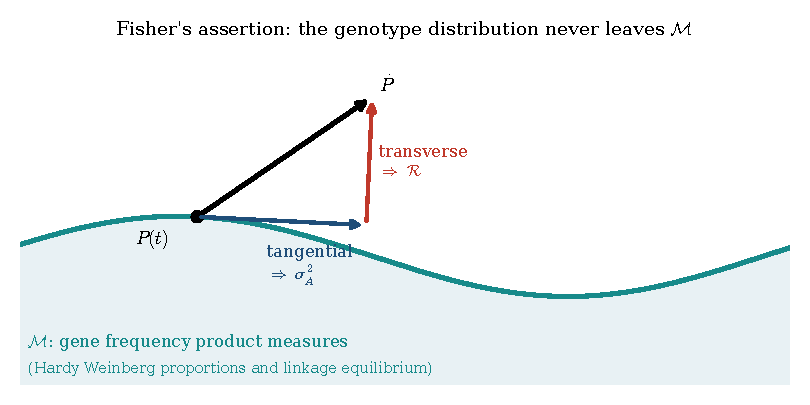
\includegraphics[width=\textwidth]{figures/ftns_f1_geometry.pdf}
\caption{The geometry of the Fundamental Theorem. The genotype distribution $P(t)$ moves in the
simplex. Its velocity decomposes into a component tangential to the manifold $\HW$ of
gene frequency product measures, which the additive genetic variance registers exactly, and a
transverse component, which it cannot see. Fisher's assertion is that the transverse component is
absent.}
\label{ftns:fig:geom}
\end{figure}

\subsection{Two questions, and the division of the chapter}

Two quite different questions arise, and confusing them has caused much of the trouble.

The first is deterministic. The Fundamental Theorem belongs to the deterministic half of
population genetics: infinitely large populations, no stochastic element, no data. In that world
one asks whether $\R=0$. The answer is no, and no data are consulted to reach it. Part I is
written in that idiom and uses statistical vocabulary only to say how its quantities could be measured.

The second is stochastic, and belongs beside the Ewens Sampling Formula rather than beside the
Fundamental Theorem. Given genomic data, what can be said about the size of the deviations
$\delta$ across a genome? This is not an interpretation of Fisher. It is the question a person
with a data set has, and it is the one on which the practical status of $\sA$ turns. Part II
addresses it.

The two come apart cleanly. Part I would be unchanged if every genome were measured without error.
Part II would be unchanged if Fisher had never written anything.

\subsection{Contributions}

\begin{enumerate}
\item \emph{A moving projection lemma} (Lemma \ref{ftns:lem:moving}): for arbitrary genotype frequency
paths, $d\mbar/dt=\sA+\sum_{u,v}\dot P_{uv}\delta_{uv}$, with $\sA$ denoting Fisher's term $2\sum_u\dot p_u\beta_u$ and with no assumption of Hardy Weinberg
proportions. The remainder is the pairing of the least squares residuals with the logarithmic
velocity of the genotype frequencies.

\item \emph{A whole genome version} (Theorem \ref{ftns:thm:whole}), with a necessary and sufficient
criterion: $\R=0$ for every assignment of fitnesses if and only if $\partial_t\log P$ lies in the
span of the gene contents, that is, if and only if the association coordinates are stationary, as they are when the distribution moves within the manifold of
product measures.

\item \emph{An identification of the transverse coordinate} with the disequilibrium coefficient
of Lindley (1988), which Section \ref{ftns:sec:lindley} shows to be the two way interaction term of the
log linear model on the genotype table, with the multilocus transverse coordinates being the
higher order interactions.

\item \emph{An exact factorization of the remainder over the transverse coordinates}
(Theorem \ref{ftns:thm:expfam}): whenever the genotype distribution moves inside an exponential family
whose main effects are the gene contents, $\R=\sum_A\langle\delta,u_A\rangle\dot\theta_A$, the
main effect directions contributing exactly zero. The number of terms is the codimension of $\HW$,
so the counting of Section \ref{ftns:sec:twoloci} is a counting of terms. At a biallelic locus the sum
has one term and evaluates to $\R=D\,\mathcal{I}(\alpha)\,\dot\alpha$, the fitness curvature times
the Fisher information about Lindley's coefficient times its velocity, with the average
effects cancelling identically (Corollary \ref{ftns:thm:lindley}). The same calculation gives the
nonadditive variance at arbitrary genotype frequencies in closed form, $\sigma^2_D=D^2\mathcal{I}(\alpha)$,
which reduces to the classical $(2pqd)^2$ under Hardy Weinberg proportions
(Proposition \ref{ftns:prop:resid}). A consequence is that Fisher's 1941
constant genic environment condition is necessary as well as sufficient for $\R=0$ at a biallelic
locus, sharpening the standard statement and supplying the statistical meaning that Ewens (2024)
reports as missing.

\item \emph{A closed form for the remainder} in discrete time at one locus with arbitrarily many
alleles (Theorem \ref{ftns:thm:main}), together with the exact two allele relative error
$Dpq/(2\wbar)$, which shows the error is $O(s)$ rather than the $O(s^2)$ one might guess
(Corollary \ref{ftns:cor:relerr}).

\item \emph{A dynamical calculation} (Section \ref{ftns:sec:qle}): at quasi linkage equilibrium the
relative error is $\epsilon\sqrt{p_Aq_Ap_Bq_B}$, independent of the recombination rate and of the
selection intensity. Recombination suppresses the disequilibrium by a factor of ten across the
range examined and suppresses the error not at all.

\item \emph{A quantitative account of nondetection}: $n^\ast\approx50\,s^{-4}$ zygotes per
genotype are needed to see the error at one locus, five billion at a one percent selection
coefficient.

\item \emph{A reformulation of Fisher's claim as $\kappa_\ell=1$}, a point mass on a shrinkage
weight, and its examination by Jeffreys's Bayes factor and by global local shrinkage.

\item \emph{Two identifications in the Bayesian apparatus}: the horseshoe places Jeffreys's
binomial prior on the shrinkage weight, with Haldane's as the improper limit of the same Beta
family; and the Ewens Sampling Formula is the marginal likelihood of a Dirichlet process prior,
with Kingman's paintbox theorem in the role of de Finetti's.

\item \emph{A prescription} for genomic practice, and an identification of the one measurement
that would settle the empirical question.
\end{enumerate}

\medskip

\noindent\emph{Plan.} Section \ref{ftns:sec:history} gives the history and the rereading in outline; the rest of the
introduction states the error and the intuition. Part I is then deterministic: the projection setup
(Section \ref{ftns:sec:setup}), the lemma and its
whole genome form (Section \ref{ftns:sec:lemma}), the Lindley coordinates and the exact factorization of the remainder
(Section \ref{ftns:sec:lindley}), the discrete closed form and two examples
(Section \ref{ftns:sec:discrete}), the quasi linkage equilibrium dynamics (Section \ref{ftns:sec:qle}), the
account of nondetection (Section \ref{ftns:sec:undetected}) and a note on terminology
(Section \ref{ftns:sec:terminology}). Part II is stochastic: the bridge (Section \ref{ftns:sec:bridge}), the
$\kappa$ formulation (Section \ref{ftns:sec:kappa}), Haldane (Section \ref{ftns:sec:haldane}), the Jeffreys
test (Section \ref{ftns:sec:jeffreys}), the horseshoe (Section \ref{ftns:sec:horseshoe}) and the sampling
formula (Section \ref{ftns:sec:esf}). Part III draws the practical consequences and gives a
prescription. Part IV places the argument in the existing literature and states a research
programme. Closing sections collect proofs, numerical verification, notation and exercises.

Because the argument of Part I is algebraic, it can be followed on small tables with a pencil, and
the chapter does this repeatedly. One locus table, a $2\times2$ genotype array with excess
homozygotes, is carried through Examples \ref{ftns:ex:ls}, \ref{ftns:ex:velocities} and
\ref{ftns:ex:lindleynum}; a two locus haplotype table off linkage equilibrium is worked in
Example \ref{ftns:ex:twolocus}; the MN blood group data supply a real Hardy Weinberg calculation in
Example \ref{ftns:ex:mn}; and Part II works a Bayes factor and a horseshoe fit through by hand in
Examples \ref{ftns:ex:assay} and \ref{ftns:ex:panel}. Every number in them was checked by
computer.

\chapterpart{The deterministic theory}

\section{A fixed subspace and a moving metric}
\label{ftns:sec:setup}

Everything in Part I concerns a deterministic system. The theory has no samples, no observations and no
random variables; where Part I mentions them, it is only to say how the quantities of the theory could be measured.

Fix a locus with alleles $A_1,\dots,A_k$. Let $P_{uv}(t)>0$ be the ordered genotype frequencies at
time $t$, with $\sum_{u,v}P_{uv}=1$ and $p_u=\sum_vP_{uv}$. \emph{No Hardy Weinberg assumption is
made.} Let $m_{uv}$ be the Malthusian parameters, fixed real numbers, and
$\mbar(t)=\sum_{u,v}P_{uv}(t)m_{uv}$.

Regard $m$ as a fixed vector in $\mathbb{R}^{k\times k}$. Let
\[
V \;=\; \big\{\,f_{uv}=c_u+c_v \ :\ c\in\mathbb{R}^k\,\big\}
\]
be the subspace of additively separable arrays. $V$ is a \emph{fixed} linear subspace: it does not
depend on $t$, on $P$, or on $m$. Equip $\mathbb{R}^{k\times k}$ with the time varying inner
product
\[
\langle f,g\rangle_t \;=\; \sum_{u,v}P_{uv}(t)\,f_{uv}g_{uv} ,
\]
and let $\Pi_t$ denote orthogonal projection onto $V$ in this inner product.

Ewens's $\beta$ definition of the average effects is exactly the statement that $\Pi_tm$ has
coefficients $\beta$: minimizing $\sum_{u,v}P_{uv}(m_{uv}-\beta_u^\ast-\beta_v^\ast)^2$ is
minimizing $\|m-f\|_t$ over $f\in V$. Write
\[
A(t) \;=\; \Pi_t m, \qquad A_{uv}=\beta_u+\beta_v, \qquad
\delta \;=\; m-A(t), \qquad \delta_{uv}=m_{uv}-\beta_u-\beta_v .
\]
The stationarity conditions are
\begin{equation}
\sum_v P_{uv}\,\delta_{uv}=0 \quad\text{for every }u ,
\qquad\text{hence}\qquad
\sum_{u,v}P_{uv}\,\delta_{uv}=0 .
\label{ftns:eq:normal}
\end{equation}

The subspace $V$ is fixed and the vector $m$ is fixed. What moves is the inner product, and
therefore the projection. This is the entire source of the difficulty, and it is a fact of linear
algebra rather than of statistics.

Three things follow, and none is stated in most textbook treatments. First, $\sA$ is an explained
sum of squares, Fisher's own 1918 decomposition applied to fitness, and it inherits every property
of such a decomposition, including dependence on the distribution of the predictors. Second, since
the weights are the current genotype frequencies, $\sA=\sA(P)$ is a functional of the state and not
a fixed genetic parameter: two populations with identical genotypic fitnesses have different
additive genetic variances and different average effects, which is Ewens's point that the $\beta$
move with the $p$; see also Lee and Chow (2013). Third, and this is the crux, the residuals are
orthogonal to gene content \emph{under $P(t)$ and under no other distribution}. Condition
\eqref{ftns:eq:normal} is a property of the fit, not of the genotypes, and treating $\sA$ as the total
change silently invokes it at a later time, where it is false.

\paragraph{The normal equations at a biallelic locus.} It helps to see the least squares problem
written out once in full. With two alleles, put $x=P_{12}=P_{21}$ for each ordered heterozygote,
so that the unordered heterozygote frequency is $2x$. The two conditions \eqref{ftns:eq:normal} read
\begin{equation}
\begin{aligned}
(2P_{11}+x)\,\beta_1+x\,\beta_2 &= P_{11}m_{11}+x\,m_{12},\\
x\,\beta_1+(2P_{22}+x)\,\beta_2 &= P_{22}m_{22}+x\,m_{12}.
\end{aligned}
\label{ftns:eq:normal2}
\end{equation}
The determinant is $(2P_{11}+x)(2P_{22}+x)-x^2=4P_{11}P_{22}+2x(P_{11}+P_{22})>0$, so the average
effects exist and are unique whenever at least two genotype classes are present. Nothing in
\eqref{ftns:eq:normal2} refers to Hardy Weinberg proportions; when they hold, the system reduces to
the familiar regression of genotypic value on gene count. The three variance components are
\[
\sigma^2_G=\sum_{u,v}P_{uv}(m_{uv}-\mbar)^2,\qquad
\sA=\sum_{u,v}P_{uv}(A_{uv}-\mbar)^2,\qquad
\sigma^2_D=\sum_{u,v}P_{uv}\delta_{uv}^2,
\]
and $\sigma^2_G=\sA+\sigma^2_D$ by Pythagoras in $\langle\cdot,\cdot\rangle_t$, the cross term
$\langle A-\mbar,\delta\rangle_t$ vanishing because $A-\mbar\in V$ and $\delta\perp V$.

\begin{example}[Average effects by weighted least squares]
\label{ftns:ex:ls}
Take a population with an excess of homozygotes, as inbreeding or population subdivision would
produce, and an overdominant fitness:
\begin{center}
\begin{tabular}{lccc}
\toprule
genotype & $A_1A_1$ & $A_1A_2$ & $A_2A_2$ \\
\midrule
frequency (unordered) & $0.30$ & $0.30$ & $0.40$ \\
Malthusian parameter $m$ & $\phantom{-}0.10$ & $\phantom{-}0.30$ & $-0.20$ \\
\bottomrule
\end{tabular}
\end{center}
So $P_{11}=0.30$, $x=0.15$, $P_{22}=0.40$, the allele frequency is $p_1=0.30+0.15=0.45$, and Hardy
Weinberg proportions at that frequency would be $(0.2025,0.4950,0.3025)$: the population is far
off the surface $\HW$. Mean fitness is $\mbar=0.03+0.09-0.08=0.04$ and the fitness curvature is
$D=m_{11}-2m_{12}+m_{22}=-0.7$.

The normal equations \eqref{ftns:eq:normal2} are
\[
0.75\,\beta_1+0.15\,\beta_2=0.075,\qquad 0.15\,\beta_1+0.95\,\beta_2=-0.035,
\]
with determinant $0.69$, so
\[
\beta_1=\frac{0.0765}{0.69}=\frac{51}{460}=0.110870,\qquad
\beta_2=-\frac{0.0375}{0.69}=-\frac{25}{460}=-0.054348 .
\]
The fitted array and the residuals are
\begin{center}
\begin{tabular}{lrrr}
\toprule
 & $A_1A_1$ & $A_1A_2$ & $A_2A_2$ \\
\midrule
$A_{uv}=\beta_u+\beta_v$ & $0.221739$ & $0.056522$ & $-0.108696$ \\
$\delta_{uv}=m_{uv}-A_{uv}$ & $-0.121739$ & $0.243478$ & $-0.091304$ \\
\bottomrule
\end{tabular}
\end{center}
and one checks \eqref{ftns:eq:normal} directly: $0.30(-0.121739)+0.15(0.243478)=0$ and
$0.15(0.243478)+0.40(-0.091304)=0$. The variance components are
\[
\sigma^2_G=0.3(0.06)^2+0.3(0.26)^2+0.4(0.24)^2=0.0444,
\]
$\sA=0.018835$ and $\sigma^2_D=0.025565$,
which add up as they should. The additive part is $42$ percent of the genetic variance.

Now hold the fitnesses and the allele frequency fixed and move the population onto $\HW$, to
$(0.2025,0.4950,0.3025)$. The average effects become $\beta=(0.155875,-0.029125)$, the additive
variance falls to $0.016941$ and the nonadditive variance rises to $0.030016$. The same alleles
with the same genotypic fitnesses have different average effects and different variance components
in the two populations. This is the second observation above in numbers: $\beta$ and $\sA$ are
functionals of the state.
\end{example}

\section{The moving projection lemma}
\label{ftns:sec:lemma}

\subsection{The lemma}

\begin{lemma}[Moving projection]
\label{ftns:lem:moving}
For arbitrary smooth genotype frequency paths $P(t)$, with $\sA$ here denoting Fisher's term $2\sum_u\dot p_u\beta_u$ (it equals the additive variance along the selection paths of Example \ref{ftns:ex:velocities}, but not for every path),
\begin{equation}
\frac{d\mbar}{dt}
\;=\;
\underbrace{\sum_{u,v}\dot P_{uv}\,A_{uv}}_{\displaystyle =\ \sA}
\;+\;
\underbrace{\sum_{u,v}\dot P_{uv}\,\delta_{uv}}_{\displaystyle =:\ \R} ,
\label{ftns:eq:lemma}
\end{equation}
and since $\sum_{u,v}P_{uv}\delta_{uv}=0$ the remainder may be written
$\R=\big\langle \delta,\ \dot P/P\big\rangle_t$, the pairing of the least squares deviations with
the logarithmic velocity of the genotype frequencies.
\end{lemma}

\begin{proof}
$\mbar=\sum_{u,v}P_{uv}m_{uv}$ with $m$ fixed, so $d\mbar/dt=\sum_{u,v}\dot P_{uv}m_{uv}$. Split
$m=A+\delta$. For the first piece,
\[
\sum_{u,v}\dot P_{uv}(\beta_u+\beta_v) = 2\sum_u\beta_u\sum_v\dot P_{uv} = 2\sum_u\beta_u\dot p_u
=\sA ,
\]
which is Ewens's Equation (2). The second piece is $\R$ by definition. The final form follows from
$\dot P_{uv}=P_{uv}\cdot(\dot P_{uv}/P_{uv})$.
\end{proof}

Nothing in the proof uses Hardy Weinberg, weak selection, one locus rather than many, or any
property of $m$. The identity is exact for arbitrary paths. Fisher asserted $d\mbar/dt=\sA$, that
is $\R=0$; equivalently he differentiated $\mbar=2\sum_up_u\beta_u$ and dropped
$2\sum_up_u\dot\beta_u$. Lemma \ref{ftns:lem:moving} says the same thing from the other side: he
computed the rate of change of $\Pi_tm$ as though $\Pi_t$ were constant.

\begin{remark}[Where the dot sits]
\label{ftns:rem:dot}
Ewens's Equation (15) writes the remainder as $2\sum_up_u\dot\beta_u$ and \eqref{ftns:eq:lemma} writes
it as $\sum_{u,v}\dot P_{uv}\delta_{uv}$. These are the same number, and the difference is only
which slot the product rule is applied in.

Since $\sum_{u,v}P_{uv}\delta_{uv}=0$, mean fitness may be written against either the fitted vector
or the original one, $\mbar=\sum_{u,v}P_{uv}A_{uv}=\sum_{u,v}P_{uv}m_{uv}$. Differentiating the
first gives two terms because both factors move,
\[
\frac{d\mbar}{dt}=\sum_{u,v}\dot P_{uv}A_{uv}+\sum_{u,v}P_{uv}\dot A_{uv}
=\sA+2\sum_u p_u\dot\beta_u ,
\]
which is Ewens's form. Differentiating the second gives only one term, because $m$ is a fixed
vector of constants and $P$ is the only thing that depends on $t$; splitting $m=A+\delta$
afterwards gives \eqref{ftns:eq:lemma}. The first terms agree, so the second terms do too.

We use the $\dot P$ form for two reasons. It differentiates only what actually moves: the
Malthusian parameters are constants and the $\beta$ are derived quantities, functions of $P$, so a
dot on $\beta$ is bookkeeping at one remove and a dot on $P$ is bookkeeping at the source. And,
more importantly, the $\dot P$ form exhibits the remainder as an inner product between $\delta$
and the velocity, which gives the vanishing criterion of Section \ref{ftns:sec:whole} immediately.
Kimura's form, Ewens's Equation (7), is a third repackaging of the same quantity, in which the transverse
coordinate $P_{uv}/(p_up_v)$ is made explicit; Lessard (1997) proved his form equal to Ewens's, and
\eqref{ftns:eq:lemma} sits between the two. Section~\ref{ftns:app:num} reports a numerical check in which
the three expressions agree to ten significant figures on a randomly chosen non Hardy Weinberg
path.
\end{remark}

\subsection{The geometry, and Kimura's coordinate}

Lemma \ref{ftns:lem:moving} makes the condition for Fisher's claim geometric rather than mysterious.
Let
\[
\HW \;=\; \big\{\,P: P_{uv}=p_up_v \ \text{for some } p\,\big\}
\]
be the Hardy Weinberg surface inside the simplex, a $(k-1)$ dimensional submanifold. Suppose
$P(t)\in\HW$ and $\dot P$ is tangential to $\HW$, so that
$\dot P_{uv}=\dot p_up_v+p_u\dot p_v$. Then
\[
\R=\sum_{u,v}(\dot p_up_v+p_u\dot p_v)\delta_{uv}
=2\sum_u\dot p_u\sum_vp_v\delta_{uv}=0
\]
by \eqref{ftns:eq:normal}. So the remainder measures exactly the component of $\dot P$ transverse to
the Hardy Weinberg surface, weighted by the deviations $\delta$.

\begin{quote}
\emph{Fisher's assertion is that the genotype frequencies move along the Hardy Weinberg
surface.} They do not: at one locus because selection on diploids perturbs the genotype
proportions, and across the genome because linkage disequilibrium is a transverse coordinate of
exactly this kind.
\end{quote}

This also explains why the theorem looks true in the simplest checks. The projection of the motion
onto $\HW$ is all that $\sA$ ever sees, and in a one locus model with Hardy Weinberg proportions
maintained by fiat there is nothing else.

Kimura's (1958) expression, Ewens's Equation (7), is
\[
\frac{d\mbar}{dt}=\sA+\sum_{u,v}p_up_v\,\delta_{uv}\,\frac{d}{dt}\!\left(\frac{P_{uv}}{p_up_v}\right),
\]
which Lessard (1997) showed equals the $2\sum p_u\dot\beta_u$ form. Lemma \ref{ftns:lem:moving} gives a
third expression for the same quantity and makes the common content visible: all three pair the
deviations $\delta$ with a measure of how the genotype frequencies move off $\HW$. Kimura's
$P_{uv}/(p_up_v)$ is the natural transverse coordinate, and its time derivative is what he pairs
with $\delta$. Section \ref{ftns:sec:lindley} identifies the invariant version of that coordinate and
computes the pairing in closed form.

The lemma is easiest to absorb by holding the state fixed and varying the velocity. Three
velocities are biologically natural, and between them they show the remainder taking every role
from nothing to everything.

\begin{example}[Three velocities through one state]
\label{ftns:ex:velocities}
Keep the population of Example \ref{ftns:ex:ls}.

\emph{Viability selection without mating}, $\dot P_{uv}=P_{uv}(m_{uv}-\mbar)$, is what happens
within a generation, or in continuous time when genotype proportions are not reset by mating. In
unordered form $\dot P=(0.018,\,0.078,\,-0.096)$ and $\dot p_1=0.018+0.039=0.057$. Then
\begin{gather*}
\frac{d\mbar}{dt}=\sum_{u,v}\dot P_{uv}m_{uv}=0.0444,\\
2\sum_u\dot p_u\beta_u=2(0.057)(0.110870+0.054348)=0.018835,
\end{gather*}
and the remainder is $\R=0.0444-0.018835=0.025565$. These are exactly $\sigma^2_G$, $\sA$ and
$\sigma^2_D$ of Example \ref{ftns:ex:ls}, and not by coincidence: with this velocity
$\sum\dot PA=\Cov_P(m,A)=\sA$ and $\R=\Cov_P(m,\delta)=\sigma^2_D$. Under pure selection the total
change is the total genetic variance and Fisher's term misses the whole of the nonadditive part,
here $58$ percent of it. Differentiating the normal equations numerically along this path gives
$\dot\beta=(0.006087,0.018261)$, so Ewens's form is
$2(0.45\times0.006087+0.55\times0.018261)=0.025565$, and Kimura's form returns the same number:
the three expressions of Remark \ref{ftns:rem:dot} agree to every printed figure.

\emph{Selection on the breeding value alone}, $\dot P_{uv}=P_{uv}(A_{uv}-\mbar)$, has
$\partial_t\log P\in V$, so the motion is tangent to the leaf through $P$ on which the association
is constant, and $\R=\langle\delta,A-\mbar\rangle_t=0$. Here $d\mbar/dt=\Cov_P(m,A)=\sA=0.018835$ and
Fisher's statement is exact.

\emph{Random mating with no selection}, $\dot P_{uv}=p_up_v-P_{uv}$, relaxes the population toward
$\HW$. In unordered form $\dot P=(-0.0975,\,0.1950,\,-0.0975)$, so $\dot p_1=0$ and the term Fisher
kept is zero. Yet
\[
\frac{d\mbar}{dt}=-0.0975(0.10)+0.1950(0.30)-0.0975(-0.20)=0.06825 ,
\]
all of it remainder: mean fitness rises because heterozygotes, the fittest class, are being
manufactured by mating, and no gene frequency records it. This is the one locus analogue of the
two locus system of Section \ref{ftns:sec:exB}, where it is recombination rather than mating that moves the population
across the surface.

A caution about what tangent means off the surface. The velocity
$\dot P_{uv}=\dot p_up_v+p_u\dot p_v$, which is tangent to $\HW$ at points \emph{of} $\HW$, is not
tangent to anything useful here: with $\dot p_1=0.057$ it gives $\R=0.002255\neq0$. Away from $\HW$
the criterion is the one of Theorem \ref{ftns:thm:whole}, $\partial_t\log P\in V$.
\end{example}

\subsection{The whole genome}
\label{ftns:sec:whole}

Ewens (2024) insists, rightly, that the Fundamental Theorem is a whole genome claim which a
one locus analysis cannot assess. Lemma \ref{ftns:lem:moving} generalizes without extra work, and the
geometric criterion becomes sharper rather than weaker.

Index the whole genome autosomal genotypes by $g$, with frequencies $P_g(t)$ and fixed Malthusian
parameters $m_g$. For each allele $A_{ij}$ let $X_{ij}(g)\in\{0,1,2\}$ be its copy number in
genotype $g$, and let
\[
V \;=\; \Big\{\, f_g=\textstyle\sum_{i,j}c_{ij}X_{ij}(g) \ :\ c\in\mathbb{R}^{\,\cdot}\,\Big\}
\]
be the span of the gene contents. Since $\sum_{i,j}X_{ij}(g)$ is twice the number of loci for every
$g$, the constants lie in $V$. Ewens's Equation (10) defines the whole genome average effects by
minimizing $\sum_gP_g\big(m_g-\sum_{(g)}\beta_{ij}\big)^2$, which is exactly the $L^2(P_t)$
projection of $m$ onto $V$, with stationarity conditions $\langle\delta,X_{ij}\rangle_t=0$ for
every allele.

\begin{theorem}[Whole genome]
\label{ftns:thm:whole}
For arbitrary genotype frequency paths $P(t)$, with no assumption of Hardy Weinberg proportions
or of linkage equilibrium,
\begin{equation}
\frac{d\mbar}{dt} \;=\; \sA \;+\; \R,
\qquad
\sA=2\sum_{i,j}\dot p_{ij}\beta_{ij},
\qquad
\R=\sum_g\dot P_g\,\delta_g=\big\langle\,\delta,\ \partial_t\log P\,\big\rangle_t .
\label{ftns:eq:whole}
\end{equation}
Moreover $\R=0$ whenever $\partial_t\log P\in V$, and if $\R=0$ for every assignment of Malthusian
parameters $m$ then necessarily $\partial_t\log P\in V$.
\end{theorem}

\begin{proof}
$d\mbar/dt=\sum_g\dot P_gm_g$ and $m=A+\delta$. For the first piece,
$A_g=\sum_{i,j}\beta_{ij}X_{ij}(g)$, so
\[
\sum_g\dot P_gA_g=\sum_{i,j}\beta_{ij}\frac{d}{dt}\sum_gP_gX_{ij}(g)
=\sum_{i,j}\beta_{ij}\frac{d}{dt}\big(2p_{ij}\big)=2\sum_{i,j}\beta_{ij}\dot p_{ij}=\sA
\]
by Ewens's Equation (11), the middle step being the definition of an allele frequency as half the
mean copy number. The second piece is $\R$, and $\dot P_g=P_g\,\partial_t\log P_g$ gives the
pairing form. If $\partial_t\log P\in V$ then $\R=0$ because $\delta\perp V$. Conversely, as $m$
ranges over $\mathbb{R}^{\,g}$ the residual $\delta$ ranges over all of $V^\perp$, so $\R=0$ for
every $m$ forces $\partial_t\log P\perp V^\perp$, that is $\partial_t\log P\in V$.
\end{proof}

The criterion has a clean reading. The set
\[
\HW\;=\;\Big\{\,P:\ \log P_g=\textstyle\sum_{i,j}c_{ij}X_{ij}(g)-\psi(c)\,\Big\}
\]
of distributions whose logarithm is additive in gene content is exactly the set of product measures
over genes, that is the genotype distributions in Hardy Weinberg proportions \emph{and} in linkage
equilibrium. It is an exponential family, and $V$ is its tangent space in exponential coordinates.
So Theorem \ref{ftns:thm:whole} says:

\begin{quote}
\emph{The additive genetic variance registers only the component of the motion tangent to
$\HW$.} Every departure from Hardy Weinberg proportions and every change in linkage
disequilibrium is transverse to $\HW$ and invisible to $\sA$.
\end{quote}

The one locus statement is the case of a single transverse coordinate; across the genome there are
as many transverse directions as there are dominance and association parameters, which is why the
failure grows worse rather than better as loci are added (Section \ref{ftns:sec:twoloci}).
Theorem \ref{ftns:thm:expfam} makes the dependence on each of them explicit. The pairing
$\langle\delta,\partial_t\log P\rangle$ in \eqref{ftns:eq:whole} is the natural duality between a
mixture coordinate residual and an exponential coordinate velocity, so the structure is the dually
flat one of information geometry (Amari, 1985). We mention this only because it makes clear that
nothing probabilistic is involved: the objects are a fixed vector, a fixed subspace and a path of
measures.

\subsection{Two remarks on interpretation}

\begin{remark}[Why the partial change has no biological interpretation]
\label{ftns:rem:partial}
Ewens (1989) introduced the partial rate of change, showed $\partial\mbar/\partial t=\sA$, and
Ewens (2024) now writes that the concept did not lead to a useful discussion because no biological
interpretation for it could be found. Lemma \ref{ftns:lem:moving} identifies the partial change as the
tangential component of the motion, which is to say the increment of a fitted projection with its
coefficients frozen at their current values. That is a property of an approximation procedure
applied to a population, not a property of the population. There is no reason for such a quantity
to have a biological meaning, and the long failure to find one is what one should expect. The
revised judgement is right, and right for a structural reason rather than as a matter of taste.
\end{remark}

\begin{remark}[The Price equation route]
\label{ftns:rem:price}
The same conclusion in one line. Apply the Price equation to the breeding value rather than to
fitness. Mendelian segregation under random mating transmits breeding value without bias, so the
transmission term vanishes and
\[
\wbar\,\Delta\bar A = \Cov_{P}(w,A) = \Cov_{P}(A+\varepsilon,A) = \Var_{P}(A) = \sA ,
\]
the middle equality being orthogonality of least squares residuals. Correctly stated, then, the
theorem concerns the mean \emph{breeding value} of fitness and not mean fitness. The two coincide
at time $t$, because the residual has mean zero there, but their increments do not. That single
substitution is the entire error, and it is worth putting to a biologist in exactly those words.
Ewens (1989, 1992) and Lessard (1997) establish the corresponding statement without random mating,
with arbitrarily many loci and under fertility selection, the average effects then being defined by
a linear system rather than by a Hardy Weinberg weighted regression; see Castilloux and Lessard
(1995) and Lessard and Castilloux (1995).
\end{remark}

\section{Lindley coordinates and an exact form for the remainder}
\label{ftns:sec:lindley}

Section \ref{ftns:sec:whole} shows that $\R$ measures transverse motion. This section identifies the
transverse coordinate, shows that the identification is forced rather than conventional, and
computes $\R$ in closed form in terms of it. The coordinate is Lindley's (1988).

\subsection{The coordinate is essentially unique}

At a biallelic locus the genotype simplex is two dimensional and $\HW$, parametrized by the allele
frequency, is one dimensional. The codimension is therefore exactly one: there is a single
transverse direction, and a single scalar coordinate on it. Any two such coordinates are functions
of one another, so the only question is which representative to use.

Lindley (1988) answers it. Writing $P_{11},P_{12},P_{22}$ for the unordered genotype frequencies,
he takes
\begin{equation}
\alpha \;=\; \log\frac{P_{11}P_{22}}{\big(\tfrac12P_{12}\big)^{2}}
\;=\; \log P_{11}-2\log\tfrac12 P_{12}+\log P_{22},
\label{ftns:eq:alpha}
\end{equation}
so that Hardy Weinberg equilibrium is $\alpha=0$, equivalently $P_{12}^2/(P_{11}P_{22})=4$. His
argument for the logarithmic scale is invariance: a condition on the simplex should be stated in a
form that does not depend on the arbitrary choice of coordinates used to describe the simplex, and
the log cross product ratio is the invariant such statement. The same argument was later formalized
in the log ratio transformations of compositional data analysis (Egozcue et al., 2003).

Three features of \eqref{ftns:eq:alpha} are worth separating.

\emph{It is the canonical parameter of an exponential family.} By Theorem \ref{ftns:thm:whole}, $\HW$ is
the set of distributions whose logarithm is additive in gene content. On a $2\times2$ genotype table
that is the log linear model with main effects only, and $\alpha$ is precisely its two way
interaction term. So the coordinate transverse to $\HW$ is the interaction parameter of a log linear
model, and $\HW$ is the subfamily obtained by setting it to zero.

\emph{It generalizes.} With $L$ biallelic loci the gamete simplex has dimension $2^L-1$ and $\HW$
has dimension $L$, so there are $2^L-1-L$ transverse coordinates: exactly the higher order
interaction terms of the log linear model on the $2^L$ table. Lindley's $\alpha$ is the same kind of coordinate for the $2\times2$ table of the two gene copies within a locus, and for $L=2$ the single between locus coordinate is the log odds ratio $\lambda$ of Section \ref{ftns:sec:twolocusex}. Within locus departures from Hardy Weinberg and between locus linkage disequilibria are the
two kinds, and the counting of Section \ref{ftns:sec:twoloci} is the counting of interaction terms.
We should flag that Lindley treated the single locus case, and that the multilocus extension,
though natural, is ours rather than his.

\emph{It is a second difference, like $D$.} Comparing \eqref{ftns:eq:alpha} with
$D=m_{11}-2m_{12}+m_{22}$, the disequilibrium coefficient is the second difference of the
log genotype \emph{frequencies} and the fitness curvature is the second difference of the genotype
\emph{fitnesses}. The two objects that meet in the remainder are the same contrast applied to the
two halves of the model.

\subsection{The remainder factorizes over the transverse coordinates}

The third observation is not a coincidence. Whenever the genotype distribution moves inside an
exponential family whose main effects are the gene contents, the remainder factorizes over the
interaction coordinates alone, and the contribution of the main effects is exactly zero.

\begin{theorem}[Exponential family factorization]
\label{ftns:thm:expfam}
Let the genotype distribution move within the family
\[
\log P_g(t) \;=\; \sum_j c_j(t)\,X_j(g) \;+\; \sum_A \theta_A(t)\,u_A(g) \;-\; \psi\big(c(t),\theta(t)\big),
\]
where $\{X_j\}$ spans $V$, the gene contents, and $\{u_A\}$ completes the basis. Then
\begin{equation}
\Big\langle \delta,\ \frac{\partial \log P}{\partial c_j}\Big\rangle_t \;=\; 0
\quad\text{for every main effect } j,
\qquad\text{and}\qquad
\R \;=\; \sum_A \big\langle \delta,\ u_A\big\rangle_t\, \dot\theta_A .
\label{ftns:eq:expfam}
\end{equation}
\end{theorem}

\begin{proof}
In an exponential family with natural parameter $\eta_k$ and sufficient statistic $T_k$,
$\partial \log P_g/\partial\eta_k=T_k(g)-\E_P T_k$. Hence
\[
\Big\langle\delta,\frac{\partial \log P}{\partial\eta_k}\Big\rangle_t
=\sum_g P_g\,\delta_g\,T_k(g)-\E_P[T_k]\sum_gP_g\delta_g
=\Cov_P(\delta,T_k)=\langle\delta,T_k\rangle_t ,
\]
using $\E_P\delta=0$ from \eqref{ftns:eq:normal}. For a main effect, $T_k=X_j$ and
$\langle\delta,X_j\rangle_t=0$ by the same stationarity conditions, which is the first claim. The
second follows by the chain rule, $\partial_t\log P=\sum_j(\partial \log P/\partial c_j)\dot c_j
+\sum_A(\partial \log P/\partial\theta_A)\dot\theta_A$, paired with $\delta$ as in
Theorem \ref{ftns:thm:whole}.
\end{proof}

Three things are worth reading off \eqref{ftns:eq:expfam}.

The remainder depends on the velocities of the interaction coordinates and on nothing else. The
allele frequencies may move as fast as they like without contributing a single term, which is
Theorem \ref{ftns:thm:whole} in differential form: $\R=0$ when $\dot\theta=0$, that is when the motion
is confined to a leaf of constant $\theta$, and to $\HW$ itself when $\theta=0$.

The number of terms in the sum is the codimension of $\HW$, namely $2^L-1-L$ on the gamete simplex of $L$ biallelic
loci. So the counting of Section \ref{ftns:sec:twoloci} is a counting of the terms in \eqref{ftns:eq:expfam},
and each transverse coordinate contributes its velocity weighted by the covariance between the
nonadditive deviation and the corresponding interaction statistic.

The weights $\langle\delta,u_A\rangle_t$ are covariances between the residual and the interaction
statistics, so a transverse coordinate contributes only insofar as the fitness deviation is
correlated with the association it measures. An epistatic interaction that no fitness deviation
tracks moves the population without moving mean fitness.

\subsection{The biallelic case in closed form}

At one locus with two alleles there is a single interaction coordinate, and evaluating
\eqref{ftns:eq:expfam} gives the whole remainder explicitly. One preliminary fact is needed first,
because the quantity that appears in the answer has a statistical identity worth fixing exactly.

\begin{lemma}[Information about Lindley's coefficient]
\label{ftns:lem:info}
In the trinomial model for unordered genotype counts, parametrized by $(p,\alpha)$ with $p$ the
allele frequency and $\alpha$ as in \eqref{ftns:eq:alpha}, the parameters are orthogonal and the
Fisher information about $\alpha$ per observation is
\begin{equation}
\mathcal{I}(\alpha)\;=\;\Big(\frac{1}{P_{11}}+\frac{4}{P_{12}}+\frac{1}{P_{22}}\Big)^{-1},
\label{ftns:eq:info}
\end{equation}
where $P_{12}$ is the unordered heterozygote frequency. Under Hardy Weinberg proportions
$\mathcal{I}(\alpha)=p^2q^2$.
\end{lemma}

\begin{proof}
Write $c=(1,-2,1)$, so $\alpha=2\log2+\sum_gc_g\log P_g$, and $h_g=c_g/P_g$. Holding $p$ fixed, the
heterozygote frequency is the only free coordinate: $P=(p-x,\,2x,\,1-p-x)$ with $x=\tfrac12P_{12}$.
Then $\partial\alpha/\partial x=-1/P_{11}-2/x-1/P_{22}=-1/\mathcal{I}(\alpha)$, so
$\partial P/\partial\alpha=-\mathcal{I}(\alpha)\,(-1,2,-1)=\mathcal{I}(\alpha)\,c$, and
\[
\sum_g\frac{(\partial P_g/\partial\alpha)^2}{P_g}=\mathcal{I}(\alpha)^2\sum_g\frac{c_g^2}{P_g}
=\mathcal{I}(\alpha)^2\cdot\frac{1}{\mathcal{I}(\alpha)}=\mathcal{I}(\alpha).
\]
For orthogonality, the cross term is
$\sum_g(\partial P_g/\partial p)(\partial P_g/\partial\alpha)/P_g
=\mathcal{I}(\alpha)\sum_g(\partial P_g/\partial p)h_g=\mathcal{I}(\alpha)\,\partial\alpha/\partial p$,
the derivative being taken at fixed $\alpha$, where it is zero. Under Hardy Weinberg
$1/p^2+4/(2pq)+1/q^2=(q+p)^2/(p^2q^2)$.
\end{proof}

Equivalently, $1/\mathcal{I}(\alpha)$ is the asymptotic variance per observation of the plug in
estimate $\hat\alpha=2\log2+\sum_gc_g\log\hat P_g$, by the delta method:
$n\Var(\hat\alpha)\to\sum_gc_g^2/P_g-(\sum_gc_g)^2=1/\mathcal{I}(\alpha)$.

\begin{corollary}[Remainder in Lindley coordinates]
\label{ftns:thm:lindley}
At a biallelic locus, parametrize the genotype simplex by $(p,\alpha)$. Then
\begin{equation}
\R \;=\; D\,\mathcal{I}(\alpha)\,\dot\alpha,
\qquad
D=m_{11}-2m_{12}+m_{22},
\label{ftns:eq:lindleyR}
\end{equation}
with $\mathcal{I}(\alpha)$ the Fisher information \eqref{ftns:eq:info}.
\end{corollary}

\begin{proof}
In the ordered array with off diagonal $x=\tfrac12P_{12}$ we have $P_{11}=p-x$, $P_{22}=1-p-x$,
and by the proof of Lemma \ref{ftns:lem:info}, $x'=\partial x/\partial\alpha=-\mathcal{I}(\alpha)$
at fixed $p$. So $\partial P/\partial\alpha$ has ordered entries $(-x',x',x',-x')$ and
\begin{align*}
\Big\langle\delta,\frac{\partial \log P}{\partial\alpha}\Big\rangle_t
&=\sum_{u,v}\delta_{uv}\frac{\partial P_{uv}}{\partial\alpha}
= x'\big(2\delta_{12}-\delta_{11}-\delta_{22}\big)\\
&= -x'\big(\delta_{11}-2\delta_{12}+\delta_{22}\big) = -x'D = D\,\mathcal{I}(\alpha) ,
\end{align*}
the average effects cancelling identically because $\delta_{uv}=m_{uv}-\beta_u-\beta_v$ and the
second difference annihilates any additively separable array. By Theorem \ref{ftns:thm:expfam} the
$p$ direction contributes nothing, so $\R$ is this weight times $\dot\alpha$.
\end{proof}

There is a second proof, shorter and more informative, because at a biallelic locus the residual
itself can be written down. The idea is that $V^\perp$ is one dimensional, so the residual is a
known vector times one number, and the second difference reads off the number.

\begin{proposition}[The residual in closed form]
\label{ftns:prop:resid}
At a biallelic locus with all three genotype classes present, let
$h=(1/P_{11},\,-2/P_{12},\,1/P_{22})$ on the unordered genotypes $A_1A_1,A_1A_2,A_2A_2$. Then $h$
spans the orthogonal complement of $V$ in $L^2(P)$, and
\begin{equation}
\delta \;=\; D\,\mathcal{I}(\alpha)\,h,
\qquad
\sigma^2_D \;=\; D^2\,\mathcal{I}(\alpha),
\qquad
\sA \;=\; \sigma^2_G-D^2\,\mathcal{I}(\alpha),
\label{ftns:eq:resid}
\end{equation}
and for every velocity $\R=\langle\delta,\dot P/P\rangle_t=D\,\mathcal{I}(\alpha)\,\dot\alpha$. Under
Hardy Weinberg proportions $\sigma^2_D=(pqD)^2$, which is the classical dominance variance
$(2pqd)^2$ in the parametrization $m=(\mu+a,\mu+d,\mu-a)$, where $D=-2d$.
\end{proposition}

\begin{proof}
Functions of the unordered genotype are functions of the gene count $n\in\{2,1,0\}$, a three
dimensional space in which $V=\operatorname{span}\{1,n\}$ has dimension two. The vector $h$ is
orthogonal to both: $\sum_gP_gh_g=1-2+1=0$ and $\sum_gP_gh_gn_g=2-2+0=0$. So $V^\perp$ is the line
through $h$ and $\delta=ch$ for some scalar $c$. Apply the second difference
$\Delta^2f=f(2)-2f(1)+f(0)$, which annihilates $V$: $\Delta^2\delta=\Delta^2m=D$, while
$\Delta^2h=1/P_{11}+4/P_{12}+1/P_{22}=1/\mathcal{I}(\alpha)$. Hence $c=D\,\mathcal{I}(\alpha)$. Then
$\sigma^2_D=c^2\sum_gP_gh_g^2=c^2/\mathcal{I}(\alpha)=D^2\mathcal{I}(\alpha)$, and
$\sA=\sigma^2_G-\sigma^2_D$ by Pythagoras. Finally
$\langle\delta,\dot P/P\rangle_t=c\sum_g\dot P_gh_g
=c\,(\dot P_{11}/P_{11}-2\dot P_{12}/P_{12}+\dot P_{22}/P_{22})=c\,\dot\alpha$. The Hardy Weinberg
case follows from Lemma \ref{ftns:lem:info}.
\end{proof}

The proposition says something the textbook formulae conceal. The dominance variance at arbitrary
genotype frequencies is the squared fitness curvature times the Fisher information about the
departure from Hardy Weinberg, and the familiar $(2pqd)^2$ is the special case in which that
information equals $p^2q^2$. Section~\ref{ftns:app:num} reports numerical confirmation of
Theorem \ref{ftns:thm:expfam} on randomly generated exponential families and of
\eqref{ftns:eq:lindleyR} across randomly drawn states and velocities.

\begin{example}[Lindley's coordinate on the worked table]
\label{ftns:ex:lindleynum}
Return to Example \ref{ftns:ex:ls}, with $(P_{11},P_{12},P_{22})=(0.30,0.30,0.40)$ and
$D=-0.7$. Lindley's coefficient is
\[
\alpha=\log\frac{0.30\times0.40}{0.15^2}=\log 5.3333=1.6740 ,
\]
well away from the Hardy Weinberg value $0$; the information is
\[
\mathcal{I}(\alpha)=\Big(\frac1{0.30}+\frac4{0.30}+\frac1{0.40}\Big)^{-1}=\frac{1}{19.1667}=0.052174,
\]
somewhat below the value $p^2q^2=0.061256$ it would take on $\HW$ at $p=0.45$. Then
$h=(3.3333,-6.6667,2.5)$ and $D\,\mathcal{I}(\alpha)=-0.036522$, so
\eqref{ftns:eq:resid} gives $\delta=(-0.121739,\,0.243478,\,-0.091304)$, the residuals of
Example \ref{ftns:ex:ls} obtained without solving any normal equations, and
$\sigma^2_D=0.49\times0.052174=0.025565$.

For the velocities of Example \ref{ftns:ex:velocities}: under selection without mating
$\dot\alpha=\Delta^2(m-\mbar)=D=-0.7$, so $\R=(-0.7)(0.052174)(-0.7)=0.025565$; under selection on
the breeding value $\dot\alpha=\Delta^2A=0$ and $\R=0$; under random mating
\begin{gather*}
\dot\alpha=\frac{-0.0975}{0.30}-2\,\frac{0.1950}{0.30}+\frac{-0.0975}{0.40}=-1.86875,\\
\R=(-0.7)(0.052174)(-1.86875)=0.06825 .
\end{gather*}
Each agrees with the direct computation. The fitness enters only through $D$; the state only
through $\mathcal{I}(\alpha)$; the motion only through $\dot\alpha$.
\end{example}

\begin{example}[Lindley's coefficient on the MN blood groups]
\label{ftns:ex:mn}
A classic sample of $1000$ people in England typed for the MN blood group, reproduced in Hartl and
Clark (2007), gave $298$ MM, $489$ MN and $213$ NN. The allele frequency is
$\hat p_M=(2\times298+489)/2000=0.5425$ and the plug in coefficient is
\[
\hat\alpha=\log\frac{0.298\times0.213}{0.2445^2}=0.0600 .
\]
By Lemma \ref{ftns:lem:info} its standard error is
$\{n\,\mathcal{I}(\hat\alpha)\}^{-1/2}=(16.2305/1000)^{1/2}=0.127$, so $\hat\alpha$ is half a
standard error from zero; the Pearson statistic is $0.22$ on one degree of freedom. The estimated
information $\mathcal{I}(\hat\alpha)=0.06161$ is indistinguishable from
$\hat p^2\hat q^2=0.06160$.

A Bayes factor in Lindley's spirit can be had in closed form. Under the alternative put a uniform
Dirichlet prior on the genotype frequencies; under Hardy Weinberg put a uniform prior on $p$. With
counts $n_{11},n_{12},n_{22}$ summing to $n$,
\[
K=\frac{2^{n_{12}}\,B(2n_{11}+n_{12}+1,\;n_{12}+2n_{22}+1)\,(n+2)!}{2\;n_{11}!\,n_{12}!\,n_{22}!},
\]
which is $K=11.3$ for these data: strong support, on Jeffreys's scale, for Hardy Weinberg proportions, and about as
much as a thousand individuals can supply under a sharp null.

What this does and does not say about the Fundamental Theorem should be kept straight. It says the
\emph{state} is close to $\HW$, so that $\mathcal{I}(\alpha)\approx p^2q^2$. It says nothing about
the \emph{velocity} $\dot\alpha$, which is what $\R$ depends on. To estimate $\dot\alpha$ one needs
two samples separated in time, and the standard error of a difference of two independent
$\hat\alpha$ at this frequency is $\sqrt2\times0.127/\sqrt{n/1000}$. Detecting a change of $0.1$ in
$\alpha$ at two standard errors therefore needs about $13{,}000$ individuals in each sample. That
is large but not absurd, which is the point of the prescription in
Section \ref{ftns:sec:prescription}: unlike the variance components, the transverse velocity is
within reach of an ordinary survey.
\end{example}

\subsection{Two loci off linkage equilibrium}
\label{ftns:sec:twolocusex}

The same construction works for any table whose transverse space is one dimensional. The simplest
multilocus case is a haploid population, or the gametic phase of a diploid one, with two biallelic
loci. Order the haplotypes $AB,Ab,aB,ab$ with frequencies $x_1,\dots,x_4$, let $n_A,n_B\in\{0,1\}$
be the gene contents, so $V=\operatorname{span}\{1,n_A,n_B\}$, and define
\begin{gather*}
\lambda=\log\frac{x_1x_4}{x_2x_3},\qquad
E=m_1-m_2-m_3+m_4,\\
\mathcal{I}(\lambda)=\Big(\sum_{i=1}^4\frac1{x_i}\Big)^{-1},\qquad
D_{AB}=x_1x_4-x_2x_3 .
\end{gather*}
Here $\lambda$ is the log odds ratio of the haplotype table, the canonical measure of linkage
disequilibrium, $E$ is the interaction contrast of fitness, and $\mathcal{I}(\lambda)$ is the
Fisher information about $\lambda$ per haplotype, by the argument of Lemma \ref{ftns:lem:info}.

\begin{proposition}[Two locus residual]
\label{ftns:prop:twolocus}
With $h=(1/x_1,-1/x_2,-1/x_3,1/x_4)$ one has $h\perp V$ in $L^2(x)$, and
\[
\delta=E\,\mathcal{I}(\lambda)\,h,\qquad \sigma^2_{AB}=E^2\,\mathcal{I}(\lambda),\qquad
\R=E\,\mathcal{I}(\lambda)\,\dot\lambda,
\]
where $\sigma^2_{AB}=\sum_ix_i\delta_i^2$ is the epistatic variance. In particular, recombination at
rate $r$ in continuous time, $\dot x=-rD_{AB}(1,-1,-1,1)$, moves no allele frequency and changes mean
fitness at the rate $\R=-r\,D_{AB}\,E$, exactly.
\end{proposition}

\begin{proof}
$\sum x_ih_i=1-1-1+1=0$, $\sum x_ih_in_A=1-1=0$ and $\sum x_ih_in_B=1-1=0$, and $V$ has codimension
one in $\mathbb{R}^4$, so $\delta=ch$. The interaction contrast annihilates $V$, so $E=c\sum_i1/x_i$
and $c=E\,\mathcal{I}(\lambda)$. The variance and the remainder follow as in
Proposition \ref{ftns:prop:resid}, with $\sum_i\dot x_ih_i=\dot\lambda$. For recombination,
$\sum_i\dot x_ih_i=-rD_{AB}\sum_i1/x_i$, so $\R=-rD_{AB}E$.
\end{proof}

\begin{example}[Tangential and transverse parts with two loci]
\label{ftns:ex:twolocus}
Take haplotype frequencies and Malthusian parameters
\begin{center}
\begin{tabular}{lcccc}
\toprule
haplotype & $AB$ & $Ab$ & $aB$ & $ab$ \\
\midrule
frequency $x$ & $0.40$ & $0.10$ & $0.20$ & $0.30$ \\
Malthusian parameter $m$ & $0.20$ & $0.00$ & $0.10$ & $0.40$ \\
\bottomrule
\end{tabular}
\end{center}
So $p_A=0.5$, $p_B=0.6$ and $D_{AB}=0.12-0.02=0.10$; linkage equilibrium would put $0.30$ rather
than $0.40$ on $AB$. Mean fitness is $\mbar=0.22$ and the interaction contrast is $E=0.5$.

\emph{Least squares.} Fitting $m\approx b_0+b_An_A+b_Bn_B$ with weights $x$ gives the normal
equations
\[
\begin{pmatrix}1&0.5&0.6\\0.5&0.5&0.4\\0.6&0.4&0.6\end{pmatrix}
\begin{pmatrix}b_0\\b_A\\b_B\end{pmatrix}
=\begin{pmatrix}0.22\\0.08\\0.10\end{pmatrix},
\qquad (b_0,b_A,b_B)=(0.32,\,-0.08,\,-0.10).
\]
The breeding values are $A=(0.14,0.24,0.22,0.32)$ and the residuals
$\delta=(0.06,-0.24,-0.12,0.08)$. Directly, $\sigma^2_G=0.0176$, $\sA=0.0056$ and
$\sigma^2_{AB}=0.0120$. Proposition \ref{ftns:prop:twolocus} gives the same residuals at once:
$\sum1/x_i=20.8333$, $\mathcal{I}(\lambda)=0.048$, $E\,\mathcal{I}(\lambda)=0.024$, and
$0.024\times(2.5,-10,-5,3.3333)=(0.06,-0.24,-0.12,0.08)$; and
$\sigma^2_{AB}=0.25\times0.048=0.012$.

Both average effects are negative, although the best haplotype $ab$ and the second best $AB$ share
no allele. At the same allele frequencies in linkage equilibrium the coefficients would be
$(0.25,-0.10,-0.05)$, with $\sA=0.0031$ and $\sigma^2_{AB}=0.015$: the average effect of $B$ halves
when nothing but the association changes.

\emph{Selection.} Under $\dot x=x(m-\mbar)$ the velocity is $(-0.008,-0.022,-0.024,0.054)$, so
$\dot p_A=-0.030$ and $\dot p_B=-0.032$. The logarithmic velocity $m-\mbar$ splits orthogonally into
a tangential part, the centred breeding value, and a transverse part, the residual:
\begin{center}
\begin{tabular}{lrrrr}
\toprule
 & $AB$ & $Ab$ & $aB$ & $ab$ \\
\midrule
$\partial_t\log x=m-\mbar$ & $-0.02$ & $-0.22$ & $-0.12$ & $0.18$ \\
tangential, $A-\mbar$ & $-0.08$ & $0.02$ & $0.00$ & $0.10$ \\
transverse, $\delta$ & $0.06$ & $-0.24$ & $-0.12$ & $0.08$ \\
\bottomrule
\end{tabular}
\end{center}
The term Fisher keeps is $b_A\dot p_A+b_B\dot p_B=0.0024+0.0032=0.0056=\sA$ (no factor two, the
organism being haploid). The remainder is $\R=\sum\dot x_i\delta_i=0.0120=\sigma^2_{AB}$, and since
$\dot\lambda=\sum_i\dot x_ih_i=E=0.5$, also $\R=0.5\times0.048\times0.5$. Fisher's term is
$32$ percent of the true rate $0.0176$.

\emph{Recombination.} Add recombination at rate $r=0.5$. Its velocity is
$-0.05\times(1,-1,-1,1)$, it moves neither allele frequency, and it contributes
$\R=-rD_{AB}E=-0.025$ to the rate of change of mean fitness. With selection and recombination
together, $d\mbar/dt=0.0176-0.025=-0.0074$: mean fitness \emph{falls}, while Fisher's term, still
$+0.0056$, says it rises. The additive variance has the wrong sign for the total, and every unit of
the discrepancy is carried by the motion of $\lambda$.
\end{example}

\subsection{What the factorization says}

Equation \eqref{ftns:eq:lindleyR} decomposes the remainder into three interpretable factors, and each
carries a separate lesson.

\paragraph{$D$: the average effects do not appear.} The fitness input is the raw second difference
of the Malthusian parameters. The $\beta$ values, which are the objects that caused all the
trouble, cancel identically. So the remainder is not a subtle functional of the fitted model; it is
the plain curvature of the fitness function, and the only reason it was ever hard to see is that
the term it belongs to was dropped.

\paragraph{$\dot\alpha$: Fisher's condition is necessary as well as sufficient.} Fisher's (1941)
constant genic environment, in the form Ewens (2024) gives as Equation (9) and read as $\sum_up_u\dot\beta_u=0$ rather than as constancy of every $\beta_u$, is exactly
$\dot\alpha=0$. Equation \eqref{ftns:eq:lindleyR} shows that at a biallelic locus this is not merely
sufficient for $\R=0$ but, whenever $D\neq0$, necessary. The theorem is exactly true when Lindley's
disequilibrium coefficient is stationary and at no other time. That sharpens the standard
statement, which gives sufficiency only, and it makes precise what Ewens and Lessard describe as
the circularity: the condition does not constrain the biology, it names the conclusion.

\paragraph{$\mathcal{I}(\alpha)$: the remainder is weighted by the information about $\alpha$.}
The middle factor is the Fisher information about the very coordinate whose motion drives the
remainder. So the remainder is large where $\alpha$ is well determined and small where it is
poorly determined. $\mathcal{I}(\alpha)$ tends to zero as any genotype class becomes rare, so
$\R\to0$ at the boundary of the simplex for any bounded $\dot\alpha$; near $\HW$ it equals $p^2q^2\le1/16$, so that
$|\R|\le|D\,\dot\alpha|/16$. The remainder is a phenomenon of intermediate frequencies, which is
where segregating variation lives, and it is exactly there that $\alpha$ is easiest to measure.
The reasons the error went unseen, collected in Section \ref{ftns:sec:undetected}, therefore do not
include any difficulty in estimating $\alpha$. They lie in $D$ and $\dot\alpha$ each being of the
order of the selection coefficient, and in the fact that nobody tried to measure $\dot\alpha$ at all.

\subsection{Consequences for measurement}

Corollary \ref{ftns:thm:lindley} converts the central question of this chapter into an estimation
problem with existing tooling, and this is the concrete content behind prescription item 9 of
Section \ref{ftns:sec:prescription}.

To know whether $\R$ matters in a given population one needs $D$, which is a fitness contrast, and
$\dot\alpha$, which is the rate of change of a function of genotype counts. The second is the hard
part only in the sense that nobody reports it. It is exactly what Lindley (1988) built inference
for, what Shoemaker, Painter and Weir (1998) extended by arguing that no population is ever exactly
in equilibrium so that the useful question is the magnitude of the departure, and what Wakefield
(2010) scaled to genome wide panels. Two time points of genotype counts at a segregating locus
suffice for a first estimate of $\dot\alpha$, with a standard error computable from
Lemma \ref{ftns:lem:info} as in Example \ref{ftns:ex:mn}; the linkage disequilibrium spectrum, and the
log odds ratio $\lambda$ of Proposition \ref{ftns:prop:twolocus}, supply the between locus analogue.

So the proposition that has been argued about since 1930 has, at a biallelic locus, the form
\emph{a measurable coefficient does not move}. Nobody needs to settle it by argument.

\section{Discrete time: a closed form, and two examples}
\label{ftns:sec:discrete}

Ewens (2024) is right that Fisher's claim is continuous time and whole genome, and that a one locus
discrete time analysis cannot settle it. What follows is offered only because it is the one place
where $\R$ can be written down explicitly and inspected.

\subsection{The closed form and its order}

Take discrete nonoverlapping generations, one locus, random mating, constant genotypic fitnesses
$w_{ij}$, so $P_t(ij)=p_ip_j$, and write $\wbar=\sum p_ip_jw_{ij}$, $w_{i\cdot}=\sum_jp_jw_{ij}$,
$\alpha_i=w_{i\cdot}-\wbar$, $\Delta p_i=p_i\alpha_i/\wbar$.

\begin{theorem}[Exact remainder, one locus, $k$ alleles]
\label{ftns:thm:main}
$$
\Delta\wbar\;=\;\frac{\sA}{\wbar}
\;+\;\frac{1}{\wbar^2}\sum_{i,j}\delta_{ij}\,(p_i\alpha_i)(p_j\alpha_j),
\qquad \delta_{ij}=w_{ij}-\wbar-\alpha_i-\alpha_j .
$$
With two alleles and $D=w_{11}-2w_{12}+w_{22}$ this is $\Delta\wbar=\sA/\wbar+D(\Delta p)^2$.
\end{theorem}

\begin{proof}
$\wbar(p)$ is an exact quadratic form in $p$, so
$\Delta\wbar=\sum_i2(\wbar+\alpha_i)\Delta p_i+\sum_{i,j}w_{ij}\Delta p_i\Delta p_j$. The first sum
is $\sA/\wbar$ since $\sum_ip_i\alpha_i=0$. In the second, put $u_i=p_i\alpha_i$ and substitute
$w_{ij}=\wbar+\alpha_i+\alpha_j+\delta_{ij}$; the terms in $\wbar$ and $\alpha$ drop because
$\sum_iu_i=0$, leaving $\wbar^{-2}\sum_{i,j}\delta_{ij}u_iu_j$.
\end{proof}

This is Ewens's Equation (16) with the neglected term supplied. In the standard parametrization
$w_{11}=\mu+a$, $w_{12}=\mu+d$, $w_{22}=\mu-a$ one has $D=-2d$ and $\R=-2d(\Delta p)^2$, so
Fisher's total change claim is exactly the hypothesis $d=0$: a sharp point null on a single
interpretable parameter. That observation is the hinge on which Part II turns.

Write $w_{ij}=1+s\,a_{ij}$. Then $D=O(s)$ and $\Delta p=O(s)$, so
\begin{equation}
\R=O(s^3), \qquad \sA/\wbar=O(s^2), \qquad
\frac{|\R|}{\sA/\wbar}=O(s) .
\label{ftns:eq:order}
\end{equation}
The relative error is first order in the selection coefficient, not second. With two alleles it
can be computed exactly, and the answer is simpler than either of its ingredients.

\begin{corollary}[Exact relative error, two alleles]
\label{ftns:cor:relerr}
At a biallelic locus under the conditions of Theorem \ref{ftns:thm:main}, with $q=1-p$,
\[
\frac{\R}{\sA/\wbar}\;=\;\frac{D\,pq}{2\,\wbar} ,
\qquad \R=D(\Delta p)^2 .
\]
\end{corollary}

\begin{proof}
Since $p\alpha_1+q\alpha_2=0$, $\alpha_2=-p\alpha_1/q$ and
$\sA=2(p\alpha_1^2+q\alpha_2^2)=2p\alpha_1^2(1+p/q)=2p\alpha_1^2/q$. With
$\Delta p=p\alpha_1/\wbar$,
\[
\frac{D(\Delta p)^2}{\sA/\wbar}=\frac{D\,p^2\alpha_1^2/\wbar^2}{2p\alpha_1^2/(q\wbar)}
=\frac{Dpq}{2\wbar}.\qedhere
\]
\end{proof}

The average excess $\alpha_1$, which carries all the dependence on the additive part of fitness,
cancels. The relative error of Fisher's term at one locus depends only on the curvature $D$, the
heterozygosity and mean fitness. With $w_{ij}=1+s\,a_{ij}$ it is $s\,|D_a|\,pq/(2\wbar)$, where
$D_a=a_{11}-2a_{12}+a_{22}$, and since $pq\le\tfrac14$ it never exceeds $s|D_a|/(8\wbar)$. For the
shape of Example \ref{ftns:ex:A} below, $D_a=-8/3$ and $pq=0.21$, so the relative error is
$0.28\,s/\wbar$ exactly, tending to $0.28\,s$ as $s\to0$ (Figure \ref{ftns:fig:order}, left panel).
At a one percent selection coefficient the theorem is wrong by about one part in $360$.

Two further consequences. The claim is false as an identity, since $\R$ vanishes for all $p$ only
when $\delta\equiv0$, which is the purely additive model. And the remainder is not sign definite:
$\R<0$ under overdominance and $\R>0$ under underdominance. At one locus with constant fitnesses
$\Delta\wbar$ is nonetheless nonnegative, but that is a separate theorem, due to Mulholland and
Smith (1959), Scheuer and Mandel (1959) and Kingman (1961), and it is a one locus phenomenon.
Conflating it with the Fundamental Theorem has done real damage, since it is true in precisely the
case everybody checks; Section \ref{ftns:sec:undetected} returns to this.

\begin{figure}[t]
\centering
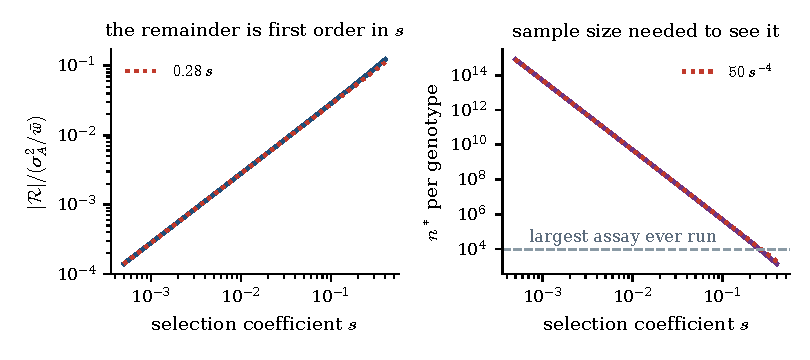
\includegraphics[width=\textwidth]{figures/ftns_f3_order.pdf}
\caption{Left: the relative error of Fisher's term is first order in the selection coefficient,
$|\R|/(\sA/\wbar)=0.28\,s$ over nearly three decades. Right: the sample size $n^\ast$ at which the
neglected term first exceeds the sampling noise in the term retained, $n^\ast\approx50\,s^{-4}$.
At a one percent selection coefficient this is five billion zygotes per genotype.}
\label{ftns:fig:order}
\end{figure}

\subsection{Example A: one locus, moderate selection}
\label{ftns:ex:A}

Take $w_{11}=0.9$, $w_{12}=1.2$, $w_{22}=0.7$ and $p_1=0.3$, so $D=-0.8$ and the heterozygote is
fittest. Then $\wbar=0.9280$, $w_{1\cdot}=1.1100$, $w_{2\cdot}=0.8500$, $\alpha_1=0.1820$,
$\alpha_2=-0.0780$ and $\Delta p=0.058836$.

\begin{center}
\begin{adjustbox}{max width=\textwidth}
\begin{tabular}{lr}
\toprule
Quantity & Value \\
\midrule
Total genetic variance $\sigma^2_G$ & $0.056616$ \\
Additive part $\sA$ & $0.028392$ \\
Nonadditive part $\sigma^2_D$ & $0.028224$ \\
\midrule
Fisher's term $\sA/\wbar$ & $\phantom{-}0.030595$ \\
Remainder $\R=D(\Delta p)^2$ & $-0.002769$ \\
Total $\Delta\wbar$ & $\phantom{-}0.027825$ \\
\bottomrule
\end{tabular}
\end{adjustbox}
\end{center}

The additive part is $50.1$ percent of the genetic variance, yet the remainder is only $9.05$
percent of Fisher's term, so his term overstates the true change by $9.95$ percent. The
9.05 percent is Corollary \ref{ftns:cor:relerr} in action: $|D|pq/(2\wbar)=0.8\times0.21/1.856=0.0905$.
By hand, $\Delta p=p\alpha_1/\wbar=0.3\times0.182/0.928=0.058836$ and
$\R=-0.8\times0.058836^2=-0.002769$, while $\sA=2(0.3\times0.182^2+0.7\times0.078^2)=0.028392$. Two percentages
are in play throughout and it is worth fixing the convention: we report
$|\R|/(\sA/\wbar)$, the remainder as a fraction of the term Fisher kept, because that is what
compares directly with the relative standard error of $\hat\sigma^2_A$ in Section \ref{ftns:sec:bias}.

The error is small because of \eqref{ftns:eq:order}: the remainder is one order higher in $s$ than the
term Fisher kept, while the quality of the fit is not. Anyone expecting a fit that explains half the
variance to produce a fifty percent error will find ten percent and conclude the theorem is fine.
At $s=0.03$ the same configuration errs by less than one percent, and at $s=0.003$ by about
one part in a thousand. What one sees is reassuring and
misleading.

\subsection{Example B: two loci, $\sA$ identically zero while mean fitness falls}
\label{ftns:sec:exB}

This is the example to put in front of a sceptic, because it removes any possibility of treating
the discrepancy as a higher order nuisance.

Two loci with alleles $A/a$ and $B/b$, gametes ordered $AB,Ab,aB,ab$ with frequencies $x$, free
recombination $r=1/2$, and
\[
w(AaBb)=w(AAbb)=w(aaBB)=1.2,\qquad\text{every other genotype}=0.6 ,
\]
with no position effect, so the coupling and repulsion double heterozygotes share the value $1.2$.
Fitness is a pure exclusive or: high when the two loci disagree. Start at
$x=(0.05,0.45,0.45,0.05)$, with the standard recursion
\[
\wbar\,x_1' = x_1(Wx)_1 - r\,w_{14}D, \qquad
\wbar\,x_2' = x_2(Wx)_2 + r\,w_{14}D, \qquad
D = x_1x_4-x_2x_3 ,
\]
and symmetrically for $x_3',x_4'$. Here $W=(w_{ij})$ is the $4\times4$ array of fitnesses of the
genotype formed by gametes $i$ and $j$, so $w_{14}=1.2$ is the fitness of the coupling double
heterozygote $AB/ab$, and $(Wx)_i=\sum_jw_{ij}x_j$ is the marginal fitness of gamete $i$.

Two facts make this example clean, and both follow from one symmetry. Let $\sigma$ exchange $A$ with
$a$ and $B$ with $b$ simultaneously. It maps the gametes $AB\leftrightarrow ab$ and
$Ab\leftrightarrow aB$, it preserves the fitness (whether the two loci disagree is unchanged), and
it preserves the state whenever $x_1=x_4$ and $x_2=x_3$. The recursion commutes with $\sigma$, so
these equalities hold in every generation, and then $p_A=x_1+x_2=\tfrac12$ and likewise
$p_B=\tfrac12$: the allele frequencies never move. Second, the weighted regression of fitness on
the gene counts $n_A,n_B$ is unique, and $\sigma$ sends $n_A\mapsto2-n_A$, $n_B\mapsto2-n_B$
while leaving fitness and weights unchanged. So if $(b_0,b_A,b_B)$ is the least squares fit then so
is $(b_0+2b_A+2b_B,-b_A,-b_B)$, and uniqueness forces $b_A=b_B=0$. Every average effect is zero,
$\sA=0$ in every generation, and Fisher's quantity predicts $\Delta\wbar=0$ forever.

\begin{center}
\begin{adjustbox}{max width=\textwidth}
\begin{tabular}{cccccc}
\toprule
Generation & $x_1=x_4$ & $x_2=x_3$ & $\wbar$ & $D$ & $\Delta\wbar$ \\
\midrule
$0$ & $0.05000$ & $0.45000$ & $1.089000$ & $-0.20000$ & $-0.153210$ \\
$1$ & $0.13912$ & $0.36088$ & $0.935790$ & $-0.11088$ & $-0.042901$ \\
$2$ & $0.17270$ & $0.32730$ & $0.892889$ & $-0.07730$ & $-0.016889$ \\
$3$ & $0.18804$ & $0.31196$ & $0.876001$ & $-0.06196$ & $-0.007558$ \\
\bottomrule
\end{tabular}
\end{adjustbox}
\end{center}

\begin{figure}[t]
\centering
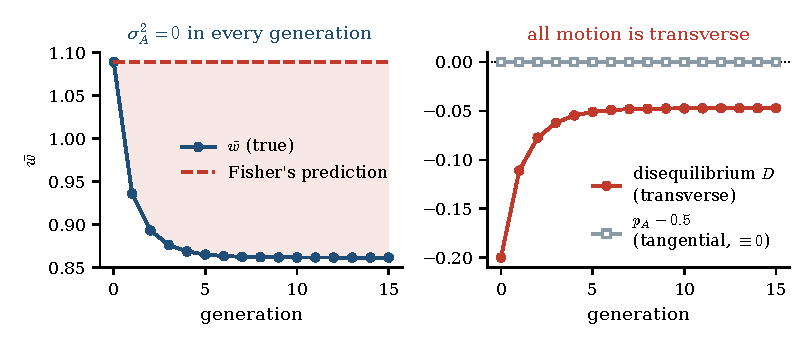
\includegraphics[width=\textwidth]{figures/ftns_f2_xor.pdf}
\caption{The exclusive or system. Mean fitness falls twenty percent (left, blue circles) while Fisher's
prediction is a flat dashed line (red), since $\sA=0$ in every generation. No allele frequency moves at
any point (right, grey open squares); the whole change is carried by the decay of linkage disequilibrium (right,
red circles), a coordinate transverse to $\HW$.}
\label{ftns:fig:xor}
\end{figure}

Mean fitness falls monotonically from $1.089$ towards $0.86$, about twenty percent, driven entirely
by the decay of linkage disequilibrium under recombination, with no allele frequency changing at
any point. In the language of Theorem \ref{ftns:thm:whole} the tangential component is identically zero
and the whole change is transverse.

The point is not that Fisher's term is inexact. In this system it carries no information at all
about the total change: it is zero while the truth is large and negative. This is the exact
complement of the Lessard and Ewens (2019) example, in which the second term does involve gene
frequency change, defeating the reading under which it is evolutionarily uninteresting; here it
involves no gene frequency change at all and yet is the entire story. Between the two, both halves
of that proposed interpretation fail. Decreases of mean fitness of this kind go back to Kojima and
Kelleher (1961) and Moran (1964).

\section{Dynamics: how far does a selected path leave the manifold?}
\label{ftns:sec:qle}

Theorem \ref{ftns:thm:whole} says $\R$ measures motion transverse to $\HW$, and Section \ref{ftns:sec:exB}
shows the transverse motion can be everything. Neither says how far an actual selected path
departs. That is a dynamical question. This section attempts it in the two locus case, and the
answer is not what one would guess.

\subsection{Setup and two findings}

Two loci, additive across loci with coefficient $s$ at each and a pure epistatic interaction of
size $\epsilon$, so that a genotype carrying $n_A$ and $n_B$ copies has fitness
\[
w \;=\; 1+s(n_A-1)+s(n_B-1)+\epsilon\,(n_A-1)(n_B-1) ,
\]
with recombination rate $r$ and no dominance within either locus, so that all nonadditivity is
epistatic. Start at linkage equilibrium and iterate. When $r\gg s$ the disequilibrium equilibrates
long before the allele frequencies move appreciably: the classical quasi linkage equilibrium
regime.

\paragraph{The disequilibrium follows the classical formula.} Measured at quasi equilibrium,
\begin{equation}
D^\ast \;=\; \frac{\epsilon\;p_Aq_A\,p_Bq_B}{r} ,
\label{ftns:eq:Dstar}
\end{equation}
confirmed numerically to within half a percent at $r=0.5$ and $r=0.25$ across $\epsilon$ from
$0.005$ to $0.02$. Tighter linkage means proportionally more disequilibrium, as one expects, and
the left panel of Figure \ref{ftns:fig:qle} shows the $1/r$ decline over a decade of $r$.

\paragraph{The relative error does not depend on $r$.} The natural defence of Fisher at this point is that recombination breaks up the associations, so
that under free recombination the epistatic remainder should be negligible. It is not.

\begin{quote}
At quasi linkage equilibrium,
\begin{equation}
\frac{|\R|}{\sA/\wbar} \;\approx\; \epsilon\,\sqrt{p_Aq_A\,p_Bq_B} ,
\label{ftns:eq:qle}
\end{equation}
with no dependence on the recombination rate $r$ and none on the selection intensity $s$.
\end{quote}

Across a grid with $s$ spanning sixteenfold ($0.0005$ to $0.008$), $\epsilon$ fourfold and $r$ from
$0.5$ to $0.2$, the ratio $|\R|/(\sA/\wbar)\div\epsilon$ stayed between $0.224$ and $0.255$ against
the predicted $p(1-p)=0.25$ at $p=\tfrac12$. Varying the allele frequency from $0.17$ to $0.84$
reproduced the $p_Aq_A$ factor with ratios $1.002$, $1.003$, $0.992$, $0.998$ and $0.998$.

\begin{figure}[t]
\centering
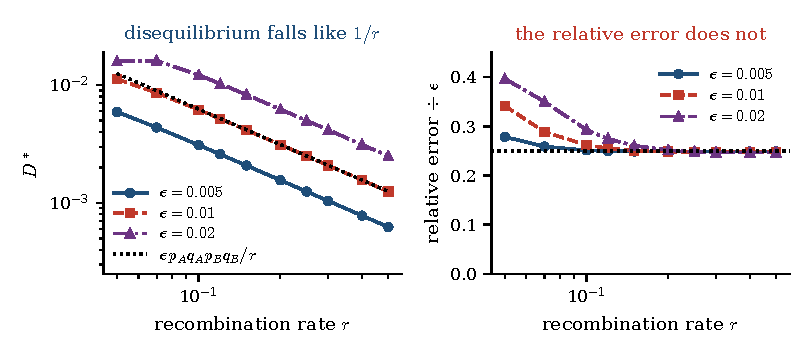
\includegraphics[width=\textwidth]{figures/ftns_f5_qle.pdf}
\caption{Quasi linkage equilibrium, $s=0.001$. Left: the disequilibrium falls like $1/r$, matching
\eqref{ftns:eq:Dstar} (dotted). Right: the relative error of Fisher's term, divided by $\epsilon$, is
flat at $p_Aq_A=0.25$ over the range where the timescales separate. Recombination removes the
disequilibrium without removing the error. The rise at $r\lesssim0.1$ is the quasi equilibrium
approximation failing.}
\label{ftns:fig:qle}
\end{figure}

\subsection{Two consequences, and caveats}

For the mathematics, \eqref{ftns:eq:qle} completes the pattern of \eqref{ftns:eq:order}. At one locus the
relative error is $0.28\,s$, first order in the selection coefficient, because the dominance
curvature there scales with $s$. Between loci it is $\epsilon\sqrt{p_Aq_Ap_Bq_B}$, first order in
the epistatic coefficient and \emph{independent of the selection intensity}. The two contributions
therefore behave differently as selection weakens: the dominance remainder vanishes with $s$ and
the epistatic remainder does not. In the weak selection limit where population genetics operates,
the epistatic contribution is the one that survives.

For the argument, this removes the most natural defence of the theorem. One expects free
recombination to protect Fisher by destroying the associations that carry the nonadditive fitness,
and the left panel of Figure \ref{ftns:fig:qle} shows that it does destroy them, by a factor of ten
across the range plotted. The right panel shows that this buys nothing. The disequilibrium falls
like $1/r$ and the error stays put, because the same recombination that suppresses $D$ also
suppresses the rate at which the population is dragged across the surface, and the two effects
cancel. There is no recombination rate at which the theorem becomes safe.

\paragraph{Caveats.} Equation \eqref{ftns:eq:qle} is verified numerically rather than derived, and we would want the
derivation before relying on it. The factor $\sqrt{p_Aq_Ap_Bq_B}$ is confirmed at $p_A=p_B$ and in
three of four asymmetric configurations tried; the fourth, at $p_A\approx0.3$ and $p_B\approx0.5$,
did not settle to the predicted value and we have not diagnosed why, though a sign change in $\R$
nearby would explain it. The model has no dominance within loci by construction, so this isolates
the epistatic contribution rather than describing a realistic architecture. And quasi linkage
equilibrium requires $r\gg s$ and $r\gg\epsilon$; the departure at small $r$ in Figure \ref{ftns:fig:qle} comes from those conditions
failing, not the formula.

\section{Why the error was not detected}
\label{ftns:sec:undetected}

The question needs rephrasing before it can be answered, because the error \emph{was} detected.
Kimura found it in 1958, and by Crow's (1987) account Fisher knew and regarded his own statement as
complete and not in need of clarification. Price found it again in 1972, Ewens in 1989 and 1992, Lessard in
1997, Lessard and Ewens in 2019; Edwards (2002) and Ewens (2004, Ch.\ 6) survey the position. So the puzzle is not detection. It is why sixty six years of
correct mathematics failed to displace the claim. The answer, we think, is that the error has
essentially no observable consequence in any regime anyone has worked in, and six separate
mechanisms conspire to make that so.

\paragraph{1. The remainder is one order smaller in the selection intensity.}
By \eqref{ftns:eq:order} the relative error is $O(s)$, and for the shape of Example \ref{ftns:ex:A} it is
$0.28\,s$ across nearly three decades:

\begin{center}
\begin{adjustbox}{max width=\textwidth}
\begin{tabular}{rrrr}
\toprule
$s$ & $\sA/\wbar$ & $\R$ & relative error \\
\midrule
$0.3$   & $3.06\times10^{-2}$ & $-2.77\times10^{-3}$ & $9.05\%$ \\
$0.1$   & $3.23\times10^{-3}$ & $-9.27\times10^{-5}$ & $2.87\%$ \\
$0.03$  & $2.86\times10^{-4}$ & $-2.42\times10^{-6}$ & $0.85\%$ \\
$0.01$  & $3.16\times10^{-5}$ & $-8.88\times10^{-8}$ & $0.28\%$ \\
\bottomrule
\end{tabular}
\end{adjustbox}
\end{center}

Selection coefficients at segregating loci are small. At one percent the theorem is wrong by about
one part in $360$, which no biologist would notice and none ought to care about.

\paragraph{2. Detecting it at one locus needs a sample of order $s^{-4}$.}
This is the decisive number. The relative standard error of $\hat\sigma^2_A$ scales as
$1/(s\sqrt n)$, because the estimator is a quadratic functional of a contrast of size $O(s)$
estimated with $O(n^{-1/2})$ noise, while the relative bias scales as $s$. Setting them equal gives
\begin{equation}
n^\ast\;\approx\;50\,s^{-4} \quad\text{zygotes per genotype.}
\label{ftns:eq:nstar}
\end{equation}

\begin{center}
\begin{adjustbox}{max width=\textwidth}
\begin{tabular}{rrr}
\toprule
$s$ & relative bias & $n^\ast$ per genotype \\
\midrule
$0.3$   & $9.05\%$   & $5.0\times10^{3}$ \\
$0.1$   & $2.87\%$   & $4.8\times10^{5}$ \\
$0.03$  & $0.85\%$   & $6.1\times10^{7}$ \\
$0.01$  & $0.28\%$   & $5.0\times10^{9}$ \\
$0.003$ & $0.084\%$  & $6.2\times10^{11}$ \\
$0.001$ & $0.028\%$  & $5.0\times10^{13}$ \\
\bottomrule
\end{tabular}
\end{adjustbox}
\end{center}

At a one percent selection coefficient one would need five billion zygotes of each genotype before
the neglected term rose above the sampling noise in the term that was kept. No viability experiment
in the history of the subject has come within five orders of magnitude of that. Fisher's error is
not merely undetected: at realistic selection intensities it is undetectable, and the fourth power
scaling means it will stay so (Figure \ref{ftns:fig:order}, right).

\paragraph{3. The standard teaching setting makes the claim exactly true.}
By Section \ref{ftns:sec:lemma}, $\R$ vanishes when the motion is tangential to the Hardy Weinberg
surface. In continuous time at one locus with Hardy Weinberg proportions imposed rather than
derived, which is how the case is almost always presented, the tangency is exact and $\R\equiv0$
identically; we verified this numerically for two to five alleles. So a reader who checks the
theorem in the setting where it is usually taught confirms it, correctly, and concludes that the
general statement is safe. The error appears only when the genotype distribution is allowed off the
surface, and the standard presentation forbids that by construction.

\paragraph{4. The proposition people actually test is a different one, and it is true.}
Ask a population geneticist to check the Fundamental Theorem and they will check whether mean
fitness increases. At one locus with constant fitnesses it does, by the theorem of Mulholland and
Smith (1959), Scheuer and Mandel (1959) and Kingman (1961), and the check succeeds every time.
Producing a failure requires two loci, recombination and epistasis together, as in
Section \ref{ftns:sec:exB} and in Kojima and Kelleher (1961) and Moran (1964). Almost nobody's working
example has all three. The monotonicity theorem thus acts as a decoy: it is true, easy to verify,
constantly mistaken for the Fundamental Theorem, and verifying it feels like verifying Fisher.

\paragraph{5. The neglected term has never been computable.}
Ewens (2024) writes that it is impossible to find explicit expressions for the whole genome average
effects, depending as they do on epistatic effects between loci and on linkage disequilibrium
values. Then $2\sum_{i,j}p_{ij}\dot\beta_{ij}$ has never been evaluated for any real system, and
could not have been. This is worth separating from the others: it is not that anyone looked at the
second term and judged it small. Nobody has ever been in a position to look at it.

\paragraph{6. Across loci the dominance contribution is small, and partly cancels.}
A genome simulation with $L=20{,}000$ segregating deleterious alleles, $w=(1,1-hs,1-s)$, selection
coefficients averaging one percent, gives a whole genome relative error from $\R$ of $0.126\%$
under directional dominance $h\sim U(0.1,0.4)$, where every $D_\ell=s_\ell(2h_\ell-1)$ is negative
so nothing cancels, and $0.059\%$ under symmetric $h\sim U(0,1)$, where about half cancels. The
cancellation is far weaker than the $\sqrt L$ a central limit heuristic would suggest, because the
sum is dominated by a handful of loci, which is the sparsity of Section \ref{ftns:sec:horseshoe} showing
up again.

That last paragraph is a caveat against Part II as much as an explanation, and we state it as such:
for \emph{dominance} at ordinary segregating loci under weak selection, the whole genome error
really is of order a tenth of a percent, and Fisher's approximation is excellent. What that
calculation excludes is exactly what Section \ref{ftns:sec:exB} and Section \ref{ftns:sec:qle} contain.
Linkage disequilibrium and epistasis are transverse coordinates too, they are not bounded by any
$O(s^3)$ argument, and by \eqref{ftns:eq:qle} they are not damped by recombination either.

\paragraph{Two further reasons that are not mathematical.}
The theorem never made a prediction. It was offered as foundational reassurance that Darwinian
selection survives Mendelian segregation, not as a tool with downstream consumers, so no
calculation ever broke in a way that would have propagated back to it. A statement that is never
used cannot be falsified by use. And the 1958 text is visibly corrupt, with many printing errors
and a plausible miscommunication with the publisher, which gives every charitable reader licence to
assume the intended statement was the correct one. Section \ref{ftns:sec:terminology} adds a third.

\section{A note on terminology}
\label{ftns:sec:terminology}

One further reason the error survived is grammatical, and it is worth separating from the
mathematics.

Consider what has to be true for the error to be easy to make and hard to notice.
Lemma \ref{ftns:lem:moving} is a product rule. Nobody forgets the product rule. What one forgets is that
something is a function of $t$ at all. And the phrase \emph{average effect of an allele} is a noun
phrase naming a property of an allele. It is grammatically an attribute, like a mass or a charge.
Read that way, $\mbar=2\sum_up_u\beta_u$ is a weighted sum of constants with moving weights, and
differentiating only the weights is not an oversight but the obvious thing to do.

Names like projection, fitted value, or least squares fit are \emph{relational}: each names
something as the output of an operation applied to a state, and each therefore carries its own time
dependence along with it. \emph{Average effect} does not. That asymmetry is not cosmetic. A noun
that conceals a functional dependence is exactly the kind of thing that survives sixty six years of
correct mathematics, and if the aim is to stop the error being repeated, it is worth naming as one
of the mechanisms by which it propagated.

\chapterpart{The stochastic theory}

\section{The bridge: a different question}
\label{ftns:sec:bridge}

Part I settles a question about a deterministic system: is $\R=0$? The answer is no, and no data
were consulted. That question is closed.

There is a second question, and it belongs on the stochastic side of population genetics, next to
the Ewens Sampling Formula rather than next to the Fundamental Theorem. Suppose one has genomic
data. What can be said about the size of the deviations $\delta$ across the genome? This is not an
interpretation of Fisher. It is the question a person with a data set has, and it is the one on
which the practical status of $\sA$ turns. Part I says $\sA$ is not the whole of $d\mbar/dt$. Part
II asks how much of it $\sA$ is, in a real genome, and what evidence could settle that.

It is worth being explicit about why the two questions do not collapse into one. Ewens's argument
solves a \emph{testing} problem: the hypothesis is $\R=0$, the loss is zero one, and the answer is
reject. A reader with a genome solves an \emph{estimation} problem: the estimand is $d\mbar/dt$,
the action is to report a number, and the loss is squared error, so that an unbiased estimator $\hat\sigma^2_A$ of $\sigma^2_A$ has risk
\[
\E\big(\hat\sigma^2_A-d\mbar/dt\big)^2 \;=\; \Var(\hat\sigma^2_A)\;+\;\R^2 .
\]
The deterministic argument fixes only that the second term is positive. It says nothing about its
size, nothing about the first term, and nothing about whether some other action has lower risk.
These are different problems and the answer to the first does not determine the answer to the
second.

\section{Fisher's $\kappa=1$ assumption}
\label{ftns:sec:kappa}

At locus $\ell$ let $\delta_\ell$ denote the nonadditive deviation and let $y_\ell$ be a
standardized estimate of it from data, scaled so that pure noise would be standard normal. Model
\begin{equation}
\begin{gathered}
\delta_\ell \mid \lambda_\ell,\tau \sim N(0,\tau^2\lambda_\ell^2),
\qquad
\kappa_\ell = \frac{1}{1+\tau^2\lambda_\ell^2} \in [0,1],
\\
\E[\delta_\ell\mid y_\ell]=(1-\E[\kappa_\ell\mid y_\ell])\,y_\ell .
\end{gathered}
\label{ftns:eq:kappa}
\end{equation}
So $\kappa_\ell=1$ shrinks the locus to exact additivity and $\kappa_\ell=0$ retains the deviation
in full. In this notation:

\begin{quote}
\emph{Fisher's assumption is $\kappa_\ell=1$ at every locus, asserted before any data.}
\end{quote}

Not that deviations are usually small, nor that they average out, but a point mass at $\kappa=1$
imposed across the whole genome. By Theorem \ref{ftns:thm:main} the two allele version is the point null
$d=0$, so the claim is a sharp hypothesis on a single interpretable parameter, and testable in the
framework Jeffreys built. Two tests follow, doing different jobs: Jeffreys's Bayes factor at one
locus (Section \ref{ftns:sec:jeffreys}) and global local shrinkage across the genome
(Section \ref{ftns:sec:horseshoe}).

\section{Haldane 1932: genetics, priors, and Fisher}
\label{ftns:sec:haldane}

Before the machinery, a historical section, because what follows is less anachronistic than it
looks. It was invented by a population geneticist of Fisher's own generation, in the same journal,
within two years of Fisher's own attack on inverse probability, and it was invented to solve a
linkage problem.

\subsection{What Haldane did}

Haldane (1932), \emph{A note on inverse probability}, opens by objecting that Bayes's theorem
assumes all values in the neighbourhood of the observed one are equally probable a priori, and
proposes to ask what more reasonable assumptions could be made. Two things come out of the note.

The first is the prior that bears his name, $\pi(\theta)\propto\{\theta(1-\theta)\}^{-1}$, or
$\text{Beta}(0,0)$. His motivation was genetic: mutation rates and rare recombination fractions
range over orders of magnitude, and a flat prior on $\theta$ asserts $\Prob(\theta<10^{-6})=10^{-6}$,
which is not a statement anyone would make about a mutation rate. Haldane's prior is flat in
$\log\{\theta/(1-\theta)\}$, so it is indifferent to the order of magnitude rather than to the
value.

The second, and for present purposes the more striking, is that his worked example is a mixture of
a point mass and a continuous density: a spike and slab, more than half a century before the term.
The example is linkage mapping in the Chinese primrose. Four hundred meioses, one hundred and sixty
crossovers, recombination fraction $\rho$. Since \emph{Primula sinensis} has twelve chromosomes of
roughly equal length and unlinked loci recombine freely, he places a point mass of $11/12$ on
$\rho=1/2$, the two loci lying on different chromosomes, and spreads the remaining $1/12$ over the
linked case.

\paragraph{Haldane's prior was cytology, not taste.} The detail worth dwelling on is where the
$11/12$ came from. It is a chromosome count: a physical fact about the organism, checkable by
anyone with a microscope, and nothing about it is subjective or convenient. That is the model
answer to the standard objection against priors, and it was produced inside genetics in the year
Fisher was arguing that inverse probability was illegitimate. Etz and Wagenmakers (2017) argue that
the conceptual step of assigning prior mass to a general law belongs to Wrinch and Jeffreys, but
that Haldane's concrete mixture was an important development, that Jeffreys knew of it, and that it
may have pushed him toward the implementation of 1935. Vogl (2017) should be read alongside: he
argues that Haldane used a flat prior in this very example, against his own stated principle.

\subsection{Why Haldane's prior is not Jeffreys's, and where both reappear}

Both are uniform, on different scales, and the scale is the entire content. Writing $I(\theta)$ for
the Fisher information of one Bernoulli trial,
\begin{gather*}
\text{Bayes Laplace: } \pi\propto1,
\qquad
\text{Jeffreys: } \pi\propto\sqrt{I(\theta)}=\{\theta(1-\theta)\}^{-1/2},
\\
\text{Haldane: } \pi\propto I(\theta)=\{\theta(1-\theta)\}^{-1}.
\end{gather*}
Jeffreys takes the square root because he wants the volume element of the Fisher Rao metric, so
his prior is flat in statistical distance and invariant under reparametrization. Haldane takes the
information itself, which is flat in the natural parameter of the exponential family, the log odds.
Haldane's posterior is $\text{Beta}(y,n-y)$, so its mean is exactly $y/n$ and there is no shrinkage
at all, at the cost of impropriety when $y=0$ or $y=n$; Jeffreys gives
$\text{Beta}(y+\tfrac12,n-y+\tfrac12)$, always proper, shrinking by half an observation at each end.

\label{ftns:sec:ladder}

This is not a digression, because the identical ladder governs the shrinkage weights of
\eqref{ftns:eq:kappa}. With $\lambda_\ell\sim C^+(0,1)$ and $\tau=1$,
\[
\kappa\ \sim\ \text{Beta}(\tfrac12,\tfrac12),
\]
which is exactly Jeffreys's prior for a binomial proportion. Simulated quantiles of $\kappa$ at
levels $0.1,0.25,0.5,0.75,0.9$ are $0.0245,0.1463,0.5002,0.8550,0.9756$ against
$\text{Beta}(\tfrac12,\tfrac12)$ values $0.0245,0.1464,0.5000,0.8536,0.9755$.

The reason this is the natural place for the invariance argument is that Jeffreys's rule applied to
the \emph{location} is useless here. For $y\sim N(\theta,1)$ we have $I(\theta)=1$, so the prior is
flat, $\E[\theta\mid y]=y$, and there is no shrinkage; in three or more dimensions it is also
inadmissible, and Jeffreys knew his rule misbehaved in multiparameter problems, which is why he
modified it to $1/\sigma$ for the normal mean and variance. The horseshoe applies the argument
instead to the shrinkage weight $\kappa$, which is a proportion: the fraction of an observation
attributed to noise. And the Jeffreys prior for a proportion is $\text{Beta}(\tfrac12,\tfrac12)$.

Within the generalized beta family (Armagan, Dunson and Clyde, 2011) the three classical binomial
priors reappear as three shrinkage rules. The Strawderman and Berger prior, which places
$\text{Beta}(\tfrac12,1)$ on $\kappa$ (Carvalho, Polson and Scott, 2010), is listed for comparison;
it has a pole at $\kappa=0$ only, so it protects large signals but has no prong at exact
additivity:

\begin{center}
\begin{tabularx}{\textwidth}{lcc>{\raggedright\arraybackslash}X}
\toprule
prior on $\kappa$ & $\Prob(\kappa<0.1)$ & $\Prob(\kappa>0.9)$ & name \\
\midrule
$\text{Beta}(1,1)$ & $0.100$ & $0.100$ & Bayes Laplace; the uniform shrinkage prior \\
$\text{Beta}(\tfrac12,1)$ & $0.316$ & $0.051$ & Strawderman (1971) and Berger \\
$\text{Beta}(\tfrac12,\tfrac12)$ & $0.205$ & $0.205$ & \emph{Jeffreys; the horseshoe} \\
$\text{Beta}(0,0)$ & $\to\tfrac12$ & $\to\tfrac12$ & \emph{Haldane}; improper \\
\bottomrule
\end{tabularx}
\end{center}

The induced tails behave accordingly: $\Prob(|\theta|>10)$ is $0.010$, $0.050$ and $0.376$ for
$\text{Beta}(1,1)$, $\text{Beta}(\tfrac12,\tfrac12)$ and $\text{Beta}(0.05,0.05)$. The horseshoe is
the Jeffreys member of the family and Haldane's is its improper limit, in which large signals are
not shrunk at all, exactly as his binomial posterior returns the maximum likelihood estimate
untouched. Figure \ref{ftns:fig:beta} plots the three densities.

\begin{figure}[t]
\centering
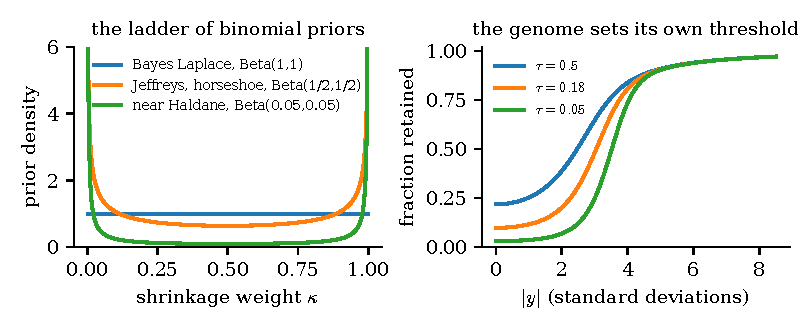
\includegraphics[width=\textwidth]{figures/ftns_f7_beta.pdf}
\caption{Left: the ladder of priors on the shrinkage weight $\kappa$ reproduces the classical
ladder of binomial priors, with the horseshoe as the Jeffreys member and Haldane's as the improper
limit. Right: the resulting shrinkage rule at three global scales. Small deviations are
erased and large ones pass through essentially untouched whatever the scale.}
\label{ftns:fig:beta}
\end{figure}

One caveat, since the correspondence is an interpretation rather than a mechanical derivation. If
one applies Jeffreys's rule literally to the marginal scale model $y\mid\kappa\sim N(0,1/\kappa)$,
the log likelihood is $\tfrac12\log\kappa-\tfrac12\kappa y^2$, so $I(\kappa)=1/(2\kappa^2)$ and
$\sqrt{I}\propto\kappa^{-1}$, which is improper and sits on the Haldane side of the horseshoe rather
than at it. The $\text{Beta}(\tfrac12,\tfrac12)$ is justified by reading $\kappa$ as an exclusion
probability, not by running the rule on the scale model, and the two readings disagree in the
direction of Haldane. The genuinely multivariate content is not in the
$\text{Beta}(\tfrac12,\tfrac12)$: it is in the shared global scale $\tau$, which lets the
coordinates borrow strength. Jeffreys's rule has no such mechanism, which is precisely where it
fails in high dimension.

\subsection{The coincidence worth noticing}

Haldane's spike and slab was built to answer the question: \emph{are these two loci linked?} It
places its point mass on $\rho=1/2$, free recombination, and its continuous part on $\rho<1/2$.

That is the same question as the one in Part I. By Theorem \ref{ftns:thm:whole} the remainder $\R$
vanishes when the motion is tangential to $\HW$, and linkage disequilibrium is exactly a transverse
coordinate; free recombination between unlinked loci is the case in which the transverse coordinate
decays fastest, and linkage is what allows it to persist. So the first mixture prior in the history
of statistics was written down to test the presence of the very structure that makes Fisher's
assertion false, by a man working in the same field. Nobody, so far as we can discover, ever joined
the two.

The chronology is worth stating plainly. Fisher (1930b) attacked inverse probability in the
\emph{Proceedings of the Cambridge Philosophical Society}. Haldane (1932) replied constructively in
the same journal with a better prior and a mixture. Fisher (1932) replied in turn, in the same
volume. Jeffreys (1935, 1936) then built the significance tests. \emph{The Genetical Theory} had
appeared in 1930 and the second edition, with the sentence at issue, in 1958. So the tools of
Section \ref{ftns:sec:jeffreys} were assembled, in Fisher's own journal and partly by a fellow
population geneticist, in the decades between the two editions of the book, and Fisher spent that
period arguing that the tools were illegitimate.

\section{The Jeffreys test: one locus, sharply}
\label{ftns:sec:jeffreys}

\subsection{The sharp null, and Jeffreys's test}

By Theorem \ref{ftns:thm:main}, $\kappa=1$ at a biallelic locus is the point null $d=0$, with $\mu$, $a$
and the error scale as nuisance parameters common to both hypotheses and so assignable improper
invariant priors without penalty. This is precisely the structure Jeffreys built his significance
tests around: a sharp null asserting that a single new parameter is absent, a diffuse alternative,
and nuisance parameters shared. Jeffreys (1935) treated the first cases; Jeffreys (1936) introduced
the notation $K$ for the ratio of posterior to prior odds on the null, with equal prior
probabilities as a working convention he was careful not to call a belief.

There is something fitting in the arrangement. Fisher's own 1918 paper supplies the variance
decomposition, Fisher's own theorem supplies the null, and the test is the one built by the
contemporary who spent a decade disputing his foundations.

If genotypic fitnesses are estimated from replicated assays with a common error variance, the
relevant statistic is the contrast
\[
\hat D = \hat w_{11}-2\hat w_{12}+\hat w_{22}, \qquad
\operatorname{se}(\hat D)^2 = \sigma^2\Big(\tfrac{1}{n_{11}}+\tfrac{4}{n_{12}}+\tfrac{1}{n_{22}}\Big),
\qquad t = \hat D/\operatorname{se}(\hat D),
\]
on $\nu$ degrees of freedom. With a Cauchy prior on the standardized dominance effect, Jeffreys's
approximation (Jeffreys, 1961; see Ly, Verhagen and Wagenmakers, 2016, for a modern account of these default tests) is
\begin{equation}
K \;\approx\; \sqrt{\tfrac{\pi\nu}{2}}\,\Big(1+\tfrac{t^2}{\nu}\Big)^{-(\nu-1)/2} .
\label{ftns:eq:jeff}
\end{equation}
Both facts that matter are visible already. The dependence on $t$ is exponential, so evidence
against additivity accumulates fast. The dependence on $\nu$ is only $\sqrt\nu$, so evidence in
favour of additivity accumulates as the square root of the sample size. \emph{A sharp null of this
kind can be destroyed but never established.} At $\nu=100$, $t=2$ gives $K=1.8$, no evidence at all
despite a conventionally significant $t$; $t=3.34$ gives $K=0.067$; $t=4.72$ gives
$K=5.9\times10^{-4}$.

\subsection{An exact binomial version, with no tuning constant}

Because a reader may object to the Cauchy scale, here is a version with no free constants. In a
viability experiment with $n$ zygotes of each genotype and $s_g\sim\text{Bin}(n,\theta_g)$,
$\theta_g$ proportional to fitness, put independent uniform priors on $\theta_{11},\theta_{22}$
under both hypotheses and set
\[
H_0: \theta_{12} = \tfrac12(\theta_{11}+\theta_{22}), \qquad
H_1: \theta_{12} \sim U(0,1) \text{ independently}.
\]
Then $K$ is a ratio of a two dimensional integral to a product of Beta functions, with no tuning
constant. Table \ref{ftns:tab:bf} evaluates it at expected data for the Example \ref{ftns:ex:A} fitnesses
rescaled to $\theta=(0.45,0.60,0.35)$ so that $d=0.20$; for a small dominance
$\theta=(0.45,0.42,0.35)$ so that $d=0.02$; and for the null itself, $\theta=(0.45,0.40,0.35)$.

\begin{table}[t]
\centering
\begin{adjustbox}{max width=\textwidth}
\begin{tabular}{rrrrr}
\toprule
& \multicolumn{2}{c}{$d=0.20$} & $d=0.02$ & $d=0$ \\
\cmidrule(lr){2-3}\cmidrule(lr){4-4}\cmidrule(lr){5-5}
$n$ per genotype & $K$ & $1/K$ & $K$ & $K$ \\
\midrule
$25$        & $9.4\times10^{-1}$  & $1.1$ & $3.4$ & $3.5$ \\
$50$        & $3.4\times10^{-1}$  & $2.9$ & $4.7$ & $4.8$ \\
$100$       & $3.2\times10^{-2}$  & $31$ & $6.4$ & $6.7$ \\
$200$       & $2.1\times10^{-4}$  & $4.9\times10^{3}$ & $8.5$ & $9.5$ \\
$400$       & $6.0\times10^{-9}$  & $1.7\times10^{8}$ & $10.7$ & $13.4$ \\
$1{,}000$   & $8.4\times10^{-23}$ & $1.2\times10^{22}$ & $12.1$ & $21.1$ \\
$4{,}000$   & $9.3\times10^{-93}$ & $1.1\times10^{92}$ & $4.6$ & $42.1$ \\
$20{,}000$  & $<10^{-300}$ & $>10^{300}$ & $1.5\times10^{-3}$ & $94.2$ \\
$100{,}000$ & $<10^{-300}$ & $>10^{300}$ & $<10^{-10}$ & $210.6$ \\
\bottomrule
\end{tabular}
\end{adjustbox}
\caption{Jeffreys's $K$ in favour of $\kappa=1$, evaluated at expected data. $K<1$ is evidence
against Fisher's assumption. Computed by windowed quadrature about the posterior mode; see
Section~\ref{ftns:app:num}.}
\label{ftns:tab:bf}
\end{table}

\begin{figure}[t]
\centering
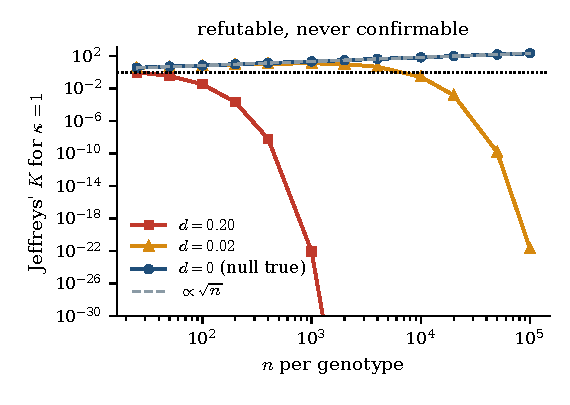
\includegraphics[width=0.7\textwidth]{figures/ftns_f6_bf.pdf}
\caption{The asymmetry of a sharp null. Under the null (blue circles) the Bayes factor grows only as
$\sqrt n$, reaching $211$ at a hundred thousand zygotes per genotype. Under a visible dominance
effect (red squares) it collapses geometrically. A small deviation (amber triangles) rises to apparent strong support
for Fisher before collapsing at sample sizes no experiment reaches.}
\label{ftns:fig:bf}
\end{figure}

The table uses expected data. It is worth doing one calculation with counts of the kind an
experiment actually produces, to see what the numbers look like in the hand.

\begin{example}[A Bayes factor from a viability assay]
\label{ftns:ex:assay}
Suppose $500$ eggs of each genotype are set up and the survivors to adulthood counted, as in a
classical \emph{Drosophila} viability assay. The counts below are illustrative, not data; they are
chosen to be typical of such assays. Three outcomes are compared, differing only in the
heterozygote:
\begin{center}
\begin{adjustbox}{max width=\textwidth}
\begin{tabular}{lccccccc}
\toprule
outcome & $s_{11}$ & $s_{12}$ & $s_{22}$ & $\hat d$ & $\hat D/\operatorname{se}(\hat D)$ & two sided $p$ & $K$ \\
\midrule
(i) overdominant & $331$ & $372$ & $302$ & $0.111$ & $-4.49$ & $7\times10^{-6}$ & $1.1\times10^{-3}$ \\
(ii) borderline & $331$ & $340$ & $302$ & $0.047$ & $-1.82$ & $0.069$ & $3.0$ \\
(iii) additive & $331$ & $318$ & $302$ & $0.003$ & $-0.11$ & $0.91$ & $15.1$ \\
\bottomrule
\end{tabular}
\end{adjustbox}
\end{center}
Here $\hat\theta_g=s_g/500$, $\hat d=\hat\theta_{12}-\tfrac12(\hat\theta_{11}+\hat\theta_{22})$,
$\hat D=\hat\theta_{11}-2\hat\theta_{12}+\hat\theta_{22}=-2\hat d$, and
$\operatorname{se}(\hat D)^2=\sum_gc_g^2\hat\theta_g(1-\hat\theta_g)/500$ with $c=(1,-2,1)$. For
outcome (i), $\hat\theta=(0.662,0.744,0.604)$, $\hat D=-0.222$ and
$\operatorname{se}(\hat D)^2=(0.2238+4\times0.1905+0.2392)/500=0.00245$, so the standardized
contrast is $-4.49$.

$K$ is the exact Bayes factor of Table \ref{ftns:tab:bf}. Under $H_1$ the marginal likelihood is
$\prod_gB(s_g+1,\,500-s_g+1)$; under $H_0$ it is the two dimensional integral
\[
\int_0^1\!\!\int_0^1\theta_{11}^{s_{11}}(1-\theta_{11})^{500-s_{11}}\,
\theta_{22}^{s_{22}}(1-\theta_{22})^{500-s_{22}}\,
\bar\theta^{\,s_{12}}(1-\bar\theta)^{500-s_{12}}\,d\theta_{11}\,d\theta_{22},
\]
where $\bar\theta=\tfrac12(\theta_{11}+\theta_{22})$;
a grid of $1600^2$ points centred on the mode evaluates it without difficulty.

Three things can be read off. Outcome (i) is decisive against additivity: posterior odds of about
$900$ to one against $\kappa=1$ from equal prior odds. Outcome (iii) is as favourable to Fisher as
data with these outer counts can be; perfectly additive data, with $s_{12}=316.5$, would give $K=15.2$, so
$15$ is the ceiling for outer counts like these at $500$ per genotype and roughly matches the $\sqrt n$ growth of the $d=0$
column of Table \ref{ftns:tab:bf}. Outcome (ii) is the Lindley (1957) phenomenon in miniature: a
contrast nearly significant at the five percent level, which a classical analyst would report as
suggestive evidence of dominance, gives odds of three to one \emph{in favour} of additivity. The
classical and Bayesian readings of the same assay point in opposite directions, and only the
second has the asymmetry of Section \ref{ftns:sec:jeffreys} built in.
\end{example}

\subsection{Three readings}

\paragraph{The asymmetry.} Where the null is exactly true, $K$ grows like $\sqrt n$: quadruple the
sample size to double the evidence, and $K=211$ at a hundred thousand zygotes per genotype, a size
no viability experiment has attained. Where dominance is present, $K$ collapses geometrically.
Lindley (1988) reported the same asymmetry in the Hardy Weinberg problem, where the Bayes factor
can favour equilibrium on data that classical tests reject. Fisher's assumption can be refuted but
not confirmed, so a century of not having refuted it is close to no evidence at all.

\paragraph{The turnover.} The $d=0.02$ column is the most instructive. A dominance effect one tenth
the size of Example \ref{ftns:ex:A}'s drives $K$ up to $12$ at $n=1000$, which on Jeffreys's scale is
strong support for $\kappa=1$, before collapsing at $n=20{,}000$. At every sample size a real
experiment uses, a small but strictly nonzero deviation masquerades as exact additivity and is
actively rewarded by the evidence. Fisher's claim is false in the manner hardest to detect: not by
a wide margin where anyone would notice, but by a small margin everywhere, accumulated over the
genome. This is the Lindley (1957) phenomenon in its natural habitat.

\paragraph{The genome wide conjunction.} Jeffreys (1936) opens by observing that independent
batches of relevant evidence multiply in their effect on the probability of the null. Fisher's
assertion requires $\kappa_\ell=1$ at every locus at once, so if
$\Prob(\kappa_\ell=1\mid\text{data})=\pi$ independently at each of $L$ loci then the posterior
probability of Fisher's claim is $\pi^L$.

\begin{center}
\begin{adjustbox}{max width=\textwidth}
\begin{tabular}{lrr}
\toprule
Per locus posterior null probability $\pi$ & $L=10^{3}$ & $L=10^{4}$ \\
\midrule
$0.90$  & $1.7\times10^{-46}$ & $<10^{-300}$ \\
$0.95$  & $5.3\times10^{-23}$ & $1.7\times10^{-223}$ \\
$0.99$  & $4.3\times10^{-5}$  & $2.2\times10^{-44}$ \\
$0.999$ & $0.37$              & $4.5\times10^{-5}$ \\
\bottomrule
\end{tabular}
\end{adjustbox}
\end{center}

Even at $\pi=0.99$ per locus, ten
thousand loci give $2.2\times10^{-44}$. Fisher's claim does not fail because some locus refutes it.
It fails because it is a conjunction of thousands of sharp nulls, and conjunctions of sharp nulls
have vanishing posterior probability under any evidence a finite experiment supplies. Wakefield
(2010) makes the corresponding point for genome wide Hardy Weinberg testing. Note that this
argument is genome wide by construction, which meets the objection that a one locus analysis cannot
settle a whole genome claim.

\subsection{An Ockham reading: Mercury and the additive model}
\label{ftns:sec:ockham}

The asymmetry of Section \ref{ftns:sec:jeffreys} has a well known reading in the philosophy of
science, and setting the two side by side sharpens what is at stake.

Jefferys and Berger (1992) give the canonical illustration.\footnote{William H.\ Jefferys, the
astronomer, is not Harold Jeffreys, whose tests Section \ref{ftns:sec:jeffreys} uses. The near homonymy
is unfortunate and is not ours.} General relativity predicts an anomalous advance of Mercury's
perihelion of $43$ arcseconds per century with no adjustable parameter; the Newtonian alternatives
of the period, an intramercurial planet or a modified inverse square exponent or an oblate sun,
could accommodate that figure but could equally have accommodated many others. The measured value
is $43.11\pm0.21$ arcseconds per century. Because the sharp theory concentrated its predictive mass
where the alternative spread it, confirmation buys an Ockham factor, the ratio of prior predictive
densities at the observed value. This is Jeffreys's simplicity postulate made quantitative, and it
is the reason a parameter free theory is worth more when it survives.

\paragraph{Fisher's claim is a Mercury type theory.} It is worth being explicit that Fisher is on
the favoured side of this argument. His assertion is the maximally sharp one available: a
parameter free identity, $\kappa_\ell=1$ at every locus, against an alternative carrying a free
sparsity level. Of the two hypotheses in Section \ref{ftns:sec:kappa} it is Fisher's that Ockham's razor
rewards, and Section \ref{ftns:sec:sparsity} says why the reward is deserved rather than accidental:
faced with $2^L-L-1$ interaction parameters, the additive model is not a convenient simplification
but the only well posed one available in 1930.

\paragraph{The reward is of the same size, and that is the problem.} A sharp null against a
diffuse alternative of prior width $\Delta$, measured with standard error $\sigma$, earns roughly
$\Delta/(\sigma\sqrt{2\pi})$ when confirmed. For Mercury, with $\sigma=0.21$ arcseconds and a prior
range of tens of arcseconds for an unexplained residual, that is a factor of order $10^2$. For the
Fundamental Theorem, the $d=0$ column of Table \ref{ftns:tab:bf} gives $K/\sqrt n$ falling from $0.69$ at $n=25$ to $0.666$ from $n=4000$ on, the Laplace limit $\{2\pi(v_{12}+\tfrac14 v_{11}+\tfrac14 v_{22})\}^{-1/2}$ with $v_g=\theta_g(1-\theta_g)$ at these null frequencies; so $K\approx0.67\sqrt n$ under the true null, and at a
hundred thousand zygotes per genotype the factor is $211$: the same order.

So the difference between the two cases is not the size of the available reward. It is that Mercury
needed the reward once and Fisher needs it $L$ times. With $\pi=K/(1+K)$ the per locus posterior
probability, the conjunction has probability $\pi^L\approx\exp(-L/K)$, so confirming it with posterior
probability one half requires $K\gtrsim L/\log2$, that is
\[
n \;\gtrsim\; \Big(\frac{L}{c\log2}\Big)^{2}, \qquad c\approx0.67,
\]
which is $4.6\times10^{6}$ at a thousand loci and $4.6\times10^{8}$ at ten thousand. At genome
scale that is about an order of magnitude below the $n^\ast\approx5\times10^{9}$ of
\eqref{ftns:eq:nstar} required to \emph{refute} the claim at a one percent selection coefficient.
The sample size at which the genome wide conjunction could first be believed and the sample size
at which its falsehood would first become visible are of comparable magnitude, and neither is
attainable.

\paragraph{What this adds.} Three things. First, it corrects a natural misreading of
Section \ref{ftns:sec:jeffreys}: the conjunction $\pi^L$ is not intrinsically hostile to a universal
claim. Had Fisher been right, the same conjunction would have delivered $K^L$ in his favour, which
is an enormous number. The conjunction is hostile only because it magnifies whichever way the
per locus evidence points, and the per locus evidence points against him.

Second, it locates precisely where Fisher's position differs from Einstein's. Both advanced a
parameter free prediction. Einstein's concerned a single observable measured to half a percent;
Fisher's concerns a latent parameter at each of $10^4$ loci, none of which any experiment reports
directly. A theory earns its Ockham reward only where its prediction is checkable, and the
Fundamental Theorem has never been anywhere that its prediction is checkable.

Third, it explains why the argument of this chapter has to be genome wide rather than
locus by locus. If the reward and the penalty both scale with $L$, then the estimand that a genome
can speak to is a functional of the distribution of $\kappa$ across loci, not the value of
$\kappa_\ell$ at any one. That is the move of Section \ref{ftns:sec:horseshoe}, and the Ockham
accounting is a second route to it.

\subsection{The Ockham factor in genetics, and in the horseshoe}
\label{ftns:sec:ockhamgen}

It is worth asking whether genetics has an equivalent of the Ockham factor. It does, in at least
two places, and in one of them the calculation has been performed daily since 1955 by people who
would decline the label.

\paragraph{Morton's LOD three.} The threshold for declaring linkage in human genetics is a LOD
score of $3$, that is a likelihood ratio of $1000$ to one. The number does not come from a
significance level. Morton (1955) derived it from prior odds: two loci chosen at random from the
genome are unlikely to be linked closely enough to detect, with prior odds of roughly $1$ in $50$,
so a likelihood ratio of $1000$ leaves posterior odds of about $20$ to one, or a posterior
probability near $0.95$. That is precisely the Ockham accounting of Section \ref{ftns:sec:ockham}, with
the prior odds supplied by genome length rather than by opinion, and it is the same calculation
Haldane (1932) made from a chromosome count twenty three years earlier. The most widely used
threshold in human genetics is a Bayes factor calibrated against a prior derived from cytology.

\paragraph{The genome wide threshold.} The modern successor is the association threshold of
$5\times10^{-8}$, which is a multiplicity correction with the same Bayesian reading: the prior odds
that a given variant is causal are of order $10^{-5}$ to $10^{-6}$, so a comparable Bayes factor is
needed before the posterior odds become respectable. Wakefield (2007) makes the translation
explicit and Stephens and Balding (2009) argue on exactly these grounds that association studies
should report Bayes factors rather than $p$ values. Churchill and Doerge's (1994) permutation
threshold, discussed in Section \ref{ftns:sec:horseshoe}, is the frequentist construction of the same
quantity.

\paragraph{MacKay's formulation, and what $\kappa$ is.} MacKay (1992, 2003) gives the Ockham factor
its standard modern form. The evidence for a model factorizes approximately as the best fit
likelihood times the ratio of the posterior accessible volume of parameter space to the prior
accessible volume, and that ratio is the penalty a model pays for having had parameters free to
adjust. A model with no adjustable parameter pays nothing; a model whose posterior has collapsed to
a small fraction of its prior range pays a great deal.

Applied to a single locus in the model of Section \ref{ftns:sec:kappa}, the calculation is exact and
identifies $\kappa$. With $y_\ell\sim N(\delta_\ell,1)$ and $\delta_\ell\mid\kappa_\ell\sim
N\big(0,(1-\kappa_\ell)/\kappa_\ell\big)$, the posterior is
$N\big((1-\kappa_\ell)y_\ell,\,1-\kappa_\ell\big)$, so
\begin{equation}
\text{Ockham factor}
\;=\;\frac{\text{posterior width}}{\text{prior width}}
\;=\;\frac{\sqrt{1-\kappa_\ell}}{\sqrt{(1-\kappa_\ell)/\kappa_\ell}}
\;=\;\sqrt{\kappa_\ell} .
\label{ftns:eq:ockhamkappa}
\end{equation}

The shrinkage weight is the squared Ockham factor. That gives Section \ref{ftns:sec:kappa} a third
reading alongside the two already offered. $\kappa_\ell$ is the fraction of the estimate discarded;
it is the exclusion probability on which Jeffreys's prior is placed (Section \ref{ftns:sec:ladder}); and
it is the square of the volume ratio by which locus $\ell$ is penalized for having had an
interaction parameter free to move.

In that third reading Fisher's assertion becomes: \emph{the Ockham factor is one at every locus in
the genome}. No interaction parameter was ever free, so none is penalized, and the additive model
pays nothing anywhere. Table \ref{ftns:tab:hs} is then an estimate of the Ockham factor genome wide, and
its finding is that the mean of $\kappa$ lies between $0.86$ and $0.98$, so the Ockham factor at
that mean shrinkage, $\sqrt{\bar\kappa}$, lies between $0.93$ and $0.99$: Fisher's model pays almost nothing at almost every locus, and pays
heavily at a few. The global scale $\hat\tau$ is the genome's own estimate of how much it should
pay in total, which is why Section \ref{ftns:sec:prescription} asks for it to be reported.

\subsection{The scale question}
\label{ftns:sec:scale}

One difficulty must be recorded. Additivity is not scale invariant, so $\kappa=1$ is not well posed
until one says on which scale. Fisher's claim concerns $m=\log w$; the discrete recursion concerns
$w$. Lindley's argument, transposed from frequencies to fitnesses, selects
$\log w_{11}-2\log w_{12}+\log w_{22}=0$, that is multiplicative fitness, equivalently additive
Malthusian parameters, which is Fisher's own scale.

This sharpens rather than repairs the failure. Put $w_{11}=c^2$, $w_{12}=c$, $w_{22}=1$, so the
invariant null holds exactly. Then
\[
D=w_{11}-2w_{12}+w_{22}=(c-1)^2>0 \quad\text{unless } c=1 ,
\]
so $\R>0$ strictly and Fisher's term now \emph{understates} the change. By
Corollary \ref{ftns:cor:relerr} the shortfall is $(c-1)^2pq/(2\wbar)$: at $c=1.5$, $p_1=0.3$ one has
$\wbar=1.3225$ and a shortfall of $0.25\times0.21/2.645=2.0$ percent, and at $c=1.25$ it is
$0.6$ percent. The two nulls are mutually exclusive except under
no selection. Jeffreys, whose programme was organized around invariance, would have raised this
before any other objection.

\section{The horseshoe test: the genome, softly}
\label{ftns:sec:horseshoe}

The sharp test cannot confirm. But Fisher's claim is not really about any single locus; it is about
the whole distribution of $\kappa$ across the genome, and that distribution \emph{is} estimable,
because information about it accumulates in the number of loci as well as in the sample size per
locus. Replace the point mass by $\lambda_\ell\sim C^+(0,1)$, which by \eqref{ftns:eq:kappa} gives
$\kappa_\ell$, at $\tau=1$, a $\text{Beta}(1/2,1/2)$ prior with unbounded density at both endpoints, and estimate
the global scale $\tau$ from all loci jointly. This is the horseshoe of Carvalho, Polson and Scott
(2010). Van der Pas, Kleijn and van der Vaart (2014) showed that its posterior contracts around a sparse mean vector at the minimax rate, up to a constant, when $\tau$ is set at about the fraction of nonzero means.

\subsection{The horseshoe in genetic terms}

Before the formulae, the picture, since the procedure is easier to justify to a geneticist than its
name suggests.

\paragraph{What $\kappa_\ell$ means at a locus.} At locus $\ell$ one has an estimated nonadditive
deviation $y_\ell$, standardized so pure noise would be standard normal. Part of it is real and
part measurement error, and one does not know the split. The weight $\kappa_\ell$ is the fraction
discarded: $\kappa_\ell=1$ throws the whole thing away and calls the locus additive,
$\kappa_\ell=0$ keeps it entire. So $\E[\kappa_\ell\mid y_\ell]$ answers the question a geneticist
actually asks: how much of this locus's apparent nonadditivity should I believe?

\paragraph{Why a prior with mass at both ends.} One wants to reach either verdict at any locus,
additive or not, without knowing in advance which loci are which. A prior concentrated in the
middle, say $\text{Beta}(5,5)$, shrinks every locus by about half, blurring the genuine epistasis
and retaining half the noise. What is wanted is weight at the two ends and little between, so the
data can push each locus to one verdict rather than leaving everything at a compromise.
$\text{Beta}(\tfrac12,\tfrac12)$ has unbounded density at $0$ and $1$ and a minimum at $\tfrac12$;
drawn, it is a horseshoe, and the two prongs are the two verdicts. Fisher's assumption keeps one
prong.

\paragraph{What $\tau$ means: a threshold the genome sets for itself.} The global scale $\tau$ is
one number estimated from all loci jointly, and it is best read as an answer to \emph{how additive
is this genome}. It fixes the effective threshold, in standard deviations, above which a locus is
allowed to keep its deviation:

\begin{center}
\begin{tabularx}{\textwidth}{>{\centering\arraybackslash}X>{\centering\arraybackslash}X>{\centering\arraybackslash}X}
\toprule
true fraction of loci nonadditive & fitted $\hat\tau$ & threshold at which half the estimate survives \\
\midrule
$0.10$ & $0.164$ & $3.09\sigma$ \\
$0.05$ & $0.072$ & $3.40\sigma$ \\
$0.02$ & $0.027$ & $3.71\sigma$ \\
$0.01$ & $0.016$ & $3.87\sigma$ \\
\bottomrule
\end{tabularx}
\end{center}

The sparser the truth, the higher the bar, and nobody chose the bar. This is the service a
permutation threshold performs in QTL mapping (Churchill and Doerge, 1994): the analyst does not
set the significance level, the genome wide distribution of the statistic sets it. The difference
is that the horseshoe does it inside the estimator rather than as a separate calibration step, and
it returns a graded weight rather than a verdict.

\paragraph{A real signal is never penalized for the company it keeps.} The rule
$\E[\delta_\ell\mid y_\ell]=(1-\E[\kappa_\ell\mid y_\ell])y_\ell$ is a soft threshold. The fraction
of the estimate retained is:

\begin{center}
\begin{adjustbox}{max width=\textwidth}
\begin{tabular}{rccc}
\toprule
$|y|$ & $\tau=0.5$ & $\tau=0.18$ & $\tau=0.05$ \\
\midrule
$0$ & $0.218$ & $0.098$ & $0.030$ \\
$2$ & $0.388$ & $0.201$ & $0.069$ \\
$3$ & $0.646$ & $0.481$ & $0.248$ \\
$4$ & $0.838$ & $0.806$ & $0.735$ \\
$6$ & $0.940$ & $0.939$ & $0.939$ \\
$8$ & $0.967$ & $0.967$ & $0.967$ \\
\bottomrule
\end{tabular}
\end{adjustbox}
\end{center}

Read the bottom rows. At six standard deviations the retained fraction is $0.94$ whatever the
global scale, and at eight it is $0.967$: a genuinely large epistatic deviation passes through
untouched even in a genome judged almost entirely additive. That is what the two prongs buy, and it
distinguishes this from ridge or lasso, which shrink a large coefficient by an amount growing with
the penalty, so a strong signal is punished for sitting among null ones. At two standard
deviations, where the winner's curse lives, between $61$ and $93$ percent is erased.
(These entries, and the thresholds above, are computed from \eqref{ftns:eq:kappapost} below; the
fitted scales are those of Table \ref{ftns:tab:hs}.)

\paragraph{What it is not.} The horseshoe is not a claim about biology and does not assert that
genomes are sparse in their epistasis. It is a statement about what one may conclude when
interaction parameters outnumber observations, and it degrades gracefully if the assumption is
wrong: a genome with pervasive epistasis of a few standard errors per locus returns a large $\hat\tau$, a low threshold and little shrinkage. (Pervasive deviations each well below their standard errors are the exception, and Section \ref{ftns:sec:omnigenic} takes them up.) Fisher's $\kappa=1$ has no such escape, returning zero whatever the genome contains.

\paragraph{How the numbers are computed.} Everything in this section follows from a single
one dimensional density. With $y_\ell\mid\delta_\ell\sim N(\delta_\ell,1)$ and the prior
\eqref{ftns:eq:kappa}, integrating out $\delta_\ell$ gives $y_\ell\mid\kappa_\ell\sim
N(0,1/\kappa_\ell)$, and combining with the induced prior on $\kappa_\ell$ (Section
\ref{ftns:app:proofs}) gives
\begin{equation}
p(\kappa\mid y,\tau)\;\propto\;\frac{e^{-\kappa y^2/2}\,(1-\kappa)^{-1/2}}{1-(1-\tau^2)\kappa},
\qquad 0<\kappa<1 .
\label{ftns:eq:kappapost}
\end{equation}
Given $\kappa$, $\delta\mid y,\kappa\sim N\big((1-\kappa)y,\,1-\kappa\big)$. So
$\E[\delta\mid y]=(1-\E[\kappa\mid y])\,y$, and
$\E[\delta^2\mid y]=\E[1-\kappa\mid y]+y^2\,\E[(1-\kappa)^2\mid y]$, each a ratio of two one
dimensional integrals; the substitution $\kappa=1-u^2$ removes the singularity at $\kappa=1$ and an
ordinary quadrature suffices. The global scale is fitted by maximizing the marginal likelihood
$\prod_\ell\int_0^1 N(y_\ell\mid0,1/\kappa)\,p(\kappa\mid\tau)\,d\kappa$ over $\tau$. Two checks are
available by hand: at $\tau=1$ and $y=0$, \eqref{ftns:eq:kappapost} is the
$\text{Beta}(1,\tfrac12)$ density, so $\E[\kappa\mid y=0]=2/3$; and as $|y|\to\infty$ the factor
$e^{-\kappa y^2/2}$ drives $\kappa$ to zero whatever $\tau$ is, which is the tail robustness above.

\begin{example}[The horseshoe on a panel of twelve loci]
\label{ftns:ex:panel}
Suppose a dominance scan of twelve loci returns the standardized contrasts in the first column
below. The values are illustrative: two loci look strongly nonadditive, two are borderline and the
rest are of the size noise produces. The table gives the posterior shrinkage weight and the
posterior mean deviation under two global scales: $\tau=0.2$, as if borrowed from a genome wide
fit, and $\hat\tau=1.02$, the marginal maximum likelihood estimate from these twelve loci alone.
\begin{center}
\begin{adjustbox}{max width=\textwidth}
\begin{tabular}{rrrrr}
\toprule
& \multicolumn{2}{c}{$\tau=0.2$} & \multicolumn{2}{c}{$\hat\tau=1.02$} \\
\cmidrule(lr){2-3}\cmidrule(lr){4-5}
$y_\ell$ & $\E[\kappa_\ell\mid y]$ & $\E[\delta_\ell\mid y]$ & $\E[\kappa_\ell\mid y]$ & $\E[\delta_\ell\mid y]$ \\
\midrule
$6.0$  & $0.061$ & $5.632$ & $0.057$ & $5.656$ \\
$4.5$  & $0.127$ & $3.929$ & $0.105$ & $4.026$ \\
$-2.7$ & $0.610$ & $-1.053$ & $0.318$ & $-1.840$ \\
$2.1$  & $0.766$ & $0.492$ & $0.445$ & $1.166$ \\
$1.6$  & $0.834$ & $0.266$ & $0.539$ & $0.738$ \\
$-1.2$ & $0.864$ & $-0.163$ & $0.595$ & $-0.486$ \\
$0.9$  & $0.878$ & $0.110$ & $0.626$ & $0.337$ \\
$-0.8$ & $0.881$ & $-0.095$ & $0.634$ & $-0.293$ \\
$0.6$  & $0.886$ & $0.068$ & $0.647$ & $0.212$ \\
$0.4$  & $0.890$ & $0.044$ & $0.656$ & $0.137$ \\
$-0.3$ & $0.891$ & $-0.033$ & $0.659$ & $-0.102$ \\
$0.1$  & $0.892$ & $0.011$ & $0.663$ & $0.034$ \\
\bottomrule
\end{tabular}
\end{adjustbox}
\end{center}
Four lessons. First, the two large contrasts are treated almost identically under the two scales:
the locus at $6.0$ keeps $94$ percent of its estimate either way. Second, the global scale decides
the fate of the middle of the table: the contrast at $-2.7$ keeps $39$ percent under $\tau=0.2$
and $68$ percent under $\hat\tau$. Third, the small contrasts are shrunk toward zero but not to it,
since the horseshoe has no point mass; under $\tau=0.2$ their weights sit near $0.89$, close to
Fisher's $\kappa=1$ but not at it. Fourth, the estimate of the nonadditive total depends on using
the right functional. Under $\tau=0.2$ the posterior mean of $\sum_\ell\delta_\ell^2$ is
$\sum_\ell\E[\delta^2_\ell\mid y]=54.2$, whereas squaring the posterior means gives
$\sum_\ell(\E[\delta_\ell\mid y])^2=48.6$; under $\hat\tau$ the two are $62.0$ and $54.0$. The
unbiased moment estimate $\sum_\ell y_\ell^2-12$ is $62.0$. Fisher's answer is $0$.

A last caution, which the genome sized calculations below remove. Twelve loci say little about
$\tau$: the marginal log likelihood is $-27.87$ at $\hat\tau$, $-28.38$ at $\tau=0.5$ and $-29.99$
at $\tau=0.2$, a likelihood ratio of about eight across a fivefold range of scales. The point of
pooling thousands of loci is to pin this one number down.
\end{example}

\subsection{What the genome says}

Table \ref{ftns:tab:hs} reports simulations with $L=5000$ loci, a fraction carrying real nonadditive
deviations, one standardized estimate per locus, and $\tau$ estimated by marginal maximum
likelihood. The target is the total nonadditive contribution $\sum_\ell\delta_\ell^2$, which is
what Fisher's second term is built out of.

\begin{table}[t]
\centering
\begin{adjustbox}{max width=\textwidth}
\begin{tabular}{ccrrrrrccc}
\toprule
\multicolumn{2}{c}{design} & \multicolumn{5}{c}{estimates of $\sum_\ell\delta^2_\ell$} &
\multicolumn{3}{c}{diagnostics} \\
\cmidrule(lr){1-2}\cmidrule(lr){3-7}\cmidrule(lr){8-10}
sparsity & sd & truth & Fisher & unshrunk & plug in & horseshoe & $\hat\tau$ &
mean $\E[\kappa\mid y]$ & top $5\%$ share \\
\midrule
$0.10$ & $3.0$ & $4766$ & $0$ & $4971$ & $3877$ & $5046$ & $0.164$ & $0.859$ & $0.966$ \\
$0.05$ & $3.0$ & $1998$ & $0$ & $1952$ & $1477$ & $2085$ & $0.072$ & $0.932$ & $0.988$ \\
$0.02$ & $2.5$ & $\phantom{0}541$ & $0$ & $\phantom{0}779$ & $\phantom{0}374$ & $\phantom{0}644$ & $0.027$ & $0.974$ & $0.993$ \\
$0.01$ & $4.0$ & $\phantom{0}623$ & $0$ & $\phantom{0}486$ & $\phantom{0}396$ & $\phantom{0}555$ & $0.016$ & $0.985$ & $0.998$ \\
\bottomrule
\end{tabular}
\end{adjustbox}
\caption{Global local shrinkage across $L=5000$ loci, one simulated genome per row: a fraction of
loci (sparsity) carries $\delta_\ell\sim N(0,\mathrm{sd}^2)$, the rest $\delta_\ell=0$, and
$y_\ell\sim N(\delta_\ell,1)$. Unshrunk is $\sum_\ell y_\ell^2-L$; plug in is
$\sum_\ell(\E[\delta_\ell\mid y])^2$; horseshoe is the posterior mean
$\sum_\ell\E[\delta_\ell^2\mid y]$ at the marginal maximum likelihood $\hat\tau$. The top five
percent share is that of the plug in total. Fisher's $\kappa=1$ forces the estimate to zero in
every row.}
\label{ftns:tab:hs}
\end{table}

\begin{figure}[t]
\centering
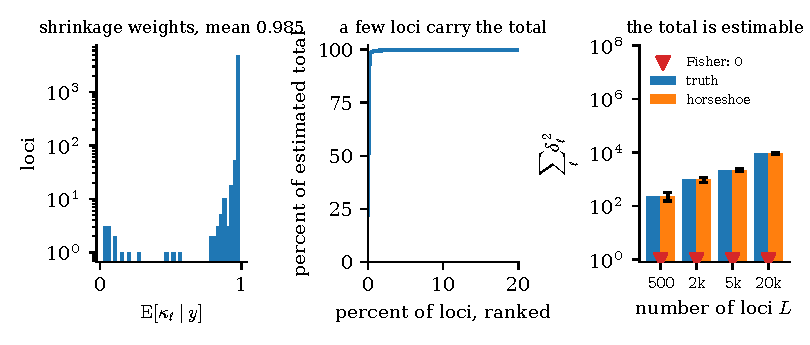
\includegraphics[width=\textwidth]{figures/ftns_f8_genome.pdf}
\caption{Genome scale behaviour. Left: the posterior shrinkage weights pile up near one, so Fisher
is nearly right at nearly every locus, but the distribution is not the point mass he assumed.
Centre: the estimated nonadditive total is concentrated in a tiny minority of loci. Right: the
aggregate against $L$, averaged over replicate genomes, with bars of one Monte Carlo standard
deviation; Fisher's answer is zero in every case.}
\label{ftns:fig:genome}
\end{figure}

Three readings, and they are the substance of the empirical test.

\paragraph{Fisher is right about most of the genome.} The posterior mean of $\kappa$ runs from
$0.86$ to $0.98$. Between eighty six and ninety eight percent of the shrinkage he imposed by
assumption is shrinkage the data endorse. His instinct about the primacy of the additive component
is not merely defensible; it is quantitatively confirmed.

\paragraph{The deviations are sparse, not absent.} The top five percent of loci carry between
$96.6$ and $99.8$ percent of the estimated nonadditive signal. This is the structure a
$\text{Beta}(1/2,1/2)$ prior on $\kappa$ is designed to represent and a point mass cannot. It is
also the reason the error is invisible locus by locus: at a randomly chosen locus Fisher is very
nearly right.

\paragraph{The aggregate is wrong by the whole quantity.} Fisher's answer for
$\sum_\ell\delta_\ell^2$ is zero, against truths between $540$ and $4800$. The horseshoe recovers
the totals to within $4$ to $19$ percent. Refusing to shrink is not the better alternative: the
unshrunk moment estimate is unbiased on average but accumulates the noise of every null locus, and
in this table it errs by $-22$ to $+44$ percent. Nor is shrinking and then squaring: the plug in
total is low in every row, by $19$ to $36$ percent, for the reason explained in
Section \ref{ftns:sec:se}. The choice is between a point mass and a prior that lets the loci speak
separately, used with the right functional.

A precedent is worth noting. Shoemaker, Painter and Weir (1998) argued that no population is ever
exactly in Hardy Weinberg equilibrium and that the useful question is the magnitude of the
departure rather than its existence. Table \ref{ftns:tab:hs} is that argument applied to $\delta$ rather
than to genotype proportions.

\subsection{Standard errors}
\label{ftns:sec:se}

Since Part I contains no standard errors by construction, the question arises only here. It divides
into a one locus sampling question and a genome wide one, and the two answer differently.

\paragraph{One locus: the standard error goes to zero and the error does not.} In a designed
viability assay with $n$ zygotes of each genotype and $s_g\sim\text{Bin}(n,\theta_g)$, the allele
frequency is fixed by the experimenter and only $\theta$ is estimated. With
$\alpha=p\theta_{11}+(q-p)\theta_{12}-q\theta_{22}$ and $\sA=2pq\alpha^2$, the delta method gives
\begin{equation}
\Var\big(\hat\sigma^2_A\big)
\;\approx\;
\frac{16p^2q^2\alpha^2}{n}\Big[p^2\theta_{11}\bar\theta_{11}+(q-p)^2\theta_{12}\bar\theta_{12}
+q^2\theta_{22}\bar\theta_{22}\Big],
\qquad \bar\theta=1-\theta .
\label{ftns:eq:delta}
\end{equation}
For Example \ref{ftns:ex:A} rescaled to $\theta=(0.45,0.60,0.35)$ with $p=0.3$, this is a relative
standard error of $638\%/\sqrt n$, confirmed by simulation to two figures: additive genetic
variance is a quadratic functional of a small contrast and correspondingly hard to pin down.
Against it sits the relative bias of $9.05\%$, which does not depend on $n$.

\begin{center}
\begin{adjustbox}{max width=\textwidth}
\begin{tabular}{rrrrr}
\toprule
$n$ per genotype & rel.\ s.e.\ (delta) & rel.\ s.e.\ (simulated) & rel.\ bias & s.e./bias \\
\midrule
$100$      & $63.8\%$ & $64.6\%$ & $9.05\%$ & $7.05$ \\
$1{,}000$  & $20.2\%$ & $20.1\%$ & $9.05\%$ & $2.23$ \\
$5{,}000$  & $9.0\%$  & $9.1\%$  & $9.05\%$ & $1.00$ \\
$10{,}000$ & $6.4\%$  & $6.3\%$  & $9.05\%$ & $0.71$ \\
$100{,}000$& $2.0\%$  & $2.1\%$  & $9.05\%$ & $0.22$ \\
\bottomrule
\end{tabular}
\end{adjustbox}
\end{center}

The mean squared error of $\hat\sigma^2_A/\wbar$ for $\Delta\wbar$ is, for large $n$, $\Var+\R^2$, the first term
$O(1/n)$ and the second fixed, with crossover at $n^\ast\approx4975$. Below it the experiment is
too noisy for anyone to have noticed; above it further data buys nothing, since what remains is
bias. Everybody worked to the left of $n^\ast$, and no standard error reveals a bias.

\paragraph{Genome wide: the aggregate is estimable, its interval needs checking.} The
quantity Fisher got wrong is the total $\sum_\ell\delta^2_\ell$, and at genome scale it behaves
better than any single locus. The table summarizes replicate genomes with five percent of loci
nonadditive, $\delta_\ell\sim N(0,9)$ there, at four genome sizes ($40$, $40$, $30$ and $20$
replicates); truth and posterior mean are averages over replicates, the Monte Carlo standard
deviation is that of the error (posterior mean minus truth), and coverage is that of the nominal
$95$ percent interval, posterior mean plus or minus $1.96$ posterior standard deviations.

\begin{center}
\begin{adjustbox}{max width=\textwidth}
\begin{tabular}{rrrrrrrr}
\toprule
$L$ & truth & posterior mean & MC s.d.\ of error & rel.\ MC s.d. & posterior s.d. & plug in bias & coverage \\
\midrule
$500$      & $233$  & $232$  & $39$  & $19.2\%$ & $32$  & $-31\%$ & $0.85$ \\
$2{,}000$  & $949$  & $970$  & $71$  & $7.8\%$  & $65$  & $-27\%$ & $0.90$ \\
$5{,}000$  & $2188$ & $2198$ & $102$ & $4.8\%$  & $99$  & $-29\%$ & $0.97$ \\
$20{,}000$ & $8876$ & $9150$ & $260$ & $3.0\%$  & $202$ & $-27\%$ & $0.60$ \\
\bottomrule
\end{tabular}
\end{adjustbox}
\end{center}

Three things follow.

First, the good news, and it is the reverse of the Jeffreys asymmetry: no single locus can confirm
$\kappa_\ell=1$ at any sample size, but the aggregate is estimated to within three percent at twenty
thousand loci, the relative error falling roughly like $L^{-1/2}$. Information about the total
accumulates in $L$ even though information about any sharp null does not.

Second, the functional matters more than the prior. The posterior mean of $\sum_\ell\delta^2_\ell$
is
\[
\sum_\ell\E[\delta_\ell^2\mid y]=\sum_\ell(\E[\delta_\ell\mid y])^2+\sum_\ell\Var(\delta_\ell\mid y),
\]
and with it the horseshoe is close to unbiased at every genome size, within three percent on
average. Squaring the posterior means and summing, the plug in that one is tempted to compute,
drops the variance term and is biased low by $27$ to $31$ percent at every $L$. The reason is
structural: a shrinkage estimator moves exactly the loci near its threshold from the mean into the
variance, and those are the loci that make up much of a quadratic total. So the plug in is a lower
bound on the nonadditive total, and the posterior mean is an estimate of it. Either way Fisher's
answer of zero is not in contention.

Third, the credible interval for the total cannot be taken on trust. Its coverage moves between $60$
and $97$ percent across the four genome sizes, and at twenty thousand loci a relative bias of three
percent is already larger than the posterior standard deviation. This is the phenomenon described
by van der Pas, Szab\'o and van der Vaart (2017): horseshoe credible sets with an adaptively chosen
sparsity level are honest only under a restriction on excessive bias, and a quadratic functional
dominated by signals near the threshold is close to the excluded case. The comparison with the
unshrunk moment estimate $\sum_\ell y_\ell^2-L$ is also instructive: here the noise variance is
known exactly, the moment estimate is unbiased, and its relative standard deviation ($22.5$, $8.4$,
$5.6$ and $2.3$ percent) is comparable to the horseshoe's, so for the total alone shrinkage buys
little when the noise model is exact. What shrinkage buys is the locus level picture of
Table \ref{ftns:tab:hs}, which the moment estimate cannot give, and robustness when per locus
standard errors must themselves be estimated. One should therefore report the horseshoe estimate of
the nonadditive total as a point estimate with a Monte Carlo or bootstrap standard error, and quote
its credible interval only after checking its coverage by simulation.

\section{The sampling theory of selectively neutral alleles}
\label{ftns:sec:esf}

This section makes explicit a structure that is present in Ewens (1972) and is usually left
unnamed.

\subsection{The sampling formula is a marginal likelihood, and the prior is forced}

The infinitely many alleles model with scaled mutation rate $\theta$ has a hierarchy with three
layers, whether or not one calls it that. The unobserved population allele frequencies, in
decreasing order, follow the Poisson Dirichlet law with parameter $\theta$, which is the law of
the ranked atoms of a Dirichlet process. Given those frequencies, a sample of $n$ genes is drawn
independently. Only the allelic partition of the sample is recorded: $a_j$ is the number of alleles represented exactly $j$ times among the $n$ genes, so that $\sum_jja_j=n$.

Integrating the second layer against the first and recording only the partition gives exactly
\[
\Prob(a_1,\dots,a_n)\;=\;\frac{n!}{\theta_{(n)}}\prod_{j=1}^{n}\frac{\theta^{a_j}}{j^{a_j}a_j!},
\qquad \theta_{(n)}=\theta(\theta+1)\cdots(\theta+n-1),
\]
the Ewens Sampling Formula. In the vocabulary of Section \ref{ftns:sec:kappa}: Poisson Dirichlet is the
prior, i.i.d.\ sampling is the likelihood, the partition is the data, $\theta$ is the
hyperparameter, and the sampling formula is the \emph{marginal likelihood} obtained by integrating
the prior out. Antoniak (1974) and Kingman (1975) set this out; Ferguson's Dirichlet process (1973)
is the same object approached from the other side.

\paragraph{Kingman's paintbox is de Finetti's theorem for partitions.} The reason this is not an accident of algebra is a representation theorem.

De Finetti's theorem says that an infinite exchangeable sequence is a mixture of independent
identically distributed sequences, and that the mixing measure is unique. The content is that
exchangeability does not permit a prior; it \emph{forces} one. A modeller who assumes his
observations are exchangeable has thereby assumed a prior, and the only remaining choice is whether
to write it down.

Kingman's paintbox theorem is the exact counterpart for exchangeable random partitions of the
integers. Every such partition is a mixture over frequency vectors $(p_1,p_2,\dots)$ with
$\sum p_i\le1$, and conditionally on the frequencies the partition arises by independent sampling
from them, with the residual mass producing singletons. The paintbox measure is the de Finetti
measure of the problem.

Apply it. Ewens (1972) assumes selectively neutral alleles with every mutation novel, that the sampled genes are exchangeable, and that only the partition is
observed. Kingman's theorem then guarantees the formula is a mixture, and identifies the mixing
measure as Poisson Dirichlet$(\theta)$. The prior was not chosen and could not have been avoided:
its existence is implied by the exchangeability and its form by the neutral model, both assumed on biological grounds, in the same way that Haldane's
$11/12$ was implied by the chromosome count.

\subsection{The estimator of $\theta$ is empirical Bayes}

The $\theta$ dependence of the sampling formula is $\theta^{K_n}/\theta_{(n)}$, where $K_n$ is the
number of distinct alleles, so $K_n$ is sufficient for $\theta$ and the maximum likelihood estimate
solves
\[
\sum_{i=0}^{n-1}\frac{\theta}{\theta+i}\;=\;k .
\]
We checked this against simulated Chinese restaurant samples: at $n=100$, $\theta=5$ the formula
gives $\E[K_n]=15.72$ against a simulated $15.76$, and a single sample with $k=15$ returns
$\hat\theta=4.66$.

That procedure is maximization of a marginal likelihood over a hyperparameter with the latent layer
integrated out. It is type II maximum likelihood, which is to say empirical Bayes, and it is the
identical operation by which $\hat\tau$ is obtained in Section \ref{ftns:sec:horseshoe}. The two
hierarchies line up term for term, as Table~\ref{ftns:tab:hierarchies} shows.

\begin{table}[tp]
\centering
\begin{tabularx}{\textwidth}{l>{\raggedright\arraybackslash}X>{\raggedright\arraybackslash}X}
\toprule
& Ewens (1972) & global local shrinkage \\
\midrule
latent layer & population allele frequencies & per locus deviations $\delta_\ell$ \\
prior & Poisson Dirichlet$(\theta)$ & scale mixture with global scale $\tau$ \\
hyperparameter & $\theta=4Nu$ & $\tau$ \\
data & allelic partition of a sample & standardized contrasts $y_\ell$ \\
marginal likelihood & the sampling formula & $\prod_\ell\int N(y_\ell\mid\delta)\pi(\delta\mid\tau)\,d\delta$ \\
hyperparameter estimate & $K_n$ sufficient, solve $\E[K_n]=k$ & marginal maximum likelihood \\
representation theorem & Kingman paintbox & de Finetti \\
\bottomrule
\end{tabularx}
\caption{The hierarchy of Ewens (1972) and the hierarchy of global local shrinkage, term by term.}\label{ftns:tab:hierarchies}
\end{table}

\subsection{Four priors already in use}

The sampling formula is the clearest instance but not the only one. Since an anti Bayesian position
is rarely a position without priors, it is worth listing the ones actually in play in this subject.
All four are justified by mechanism rather than taste, which is what makes them invisible.

\paragraph{The additive subspace.} The sharpest, because it sits inside the Fundamental Theorem
itself. The average effects are defined by minimizing $\sum_{u,v}P_{uv}(m_{uv}-b_u-b_v)^2$, a
projection onto the space of functions additive in gene content. Nothing forces that subspace: out
of $2^L$ dimensions it selects $L+1$ and discards every interaction coordinate before any data
are seen. The justification is biological, namely that genes are transmitted singly and segregation
dismantles the rest. That is a good reason and it is precisely a prior justified by mechanism.
Fisher's error was to promote it to a theorem, not to have selected it, but selected it was.

\paragraph{Exchangeability and the neutral model, which force Poisson Dirichlet.} As above.

\paragraph{The measure hiding in \emph{generically nonzero}.} The claim that the second term of
\eqref{ftns:eq:split} is not in general zero is, as mathematics, unimpeachable: the zero set of a
nontrivial analytic function has Lebesgue measure zero. But the step from \emph{the exceptions have
measure zero} to \emph{therefore this matters for real populations} requires that populations do
not sit in or near the exceptional set, and that is a claim about where organisms live rather than
a theorem. It is not idle: the exceptional set contains the one locus continuous time case with
Hardy Weinberg proportions maintained, where $\R\equiv0$ exactly, and $\R$ stays small, only $0.28\,s$ of Fisher's term, in a large
neighbourhood of it.

\paragraph{Conditioning on $K$ rather than integrating $\theta$ out.} The Ewens Watterson test
uses the sampling formula conditional on the number of alleles, because that conditional is free of
$\theta$. We verified it: at $n=8$ and $K=3$ the conditional distribution over partitions is
$(0.255864,0.307036,0.255864,0.095949,0.085288)$ at $\theta=0.5$, at $\theta=2$ and at $\theta=10$,
identical to six figures. That is disposal of a nuisance parameter by conditioning on a sufficient
statistic; a Bayesian disposes of the same parameter by integration. The two routes differ in
tactics and both require the same three layer hierarchy to be in place first.

The pattern is that an anti Bayesian practice is rarely one without priors, but one whose priors
are so well motivated that nobody calls them priors: genes transmitted singly, mutations always
novel, samples exchangeable, chromosomes countable. These are Haldane's kind, derived from mechanism
and checkable against the organism. Worth adding is where no prior is used at all, and rightly: the
refutation itself requires no measure on anything, which is why Part I is written without one.

\subsection{Pooling is not a Bayesian imposition}

Equation \eqref{ftns:eq:nstar} says the sample sizes needed to estimate small selective differences
locus by locus are impossible. One might conclude that the topic goes nowhere. The conclusion does
not follow, and the reason is the point of a hierarchical model. Pooling across loci rests on three
independent legs, only one of which is Bayesian.

\emph{De Finetti.} If, before seeing the data, one has no reason to single out any particular
locus, the per locus deviations are exchangeable, and the representation theorem says they are
conditionally independent draws from a common distribution $G$. The hierarchical model is not an
assumption added on top; it is what exchangeability means. The same move was accepted in 1972 for
genes.

\emph{Stein.} For three or more parallel estimation problems (James and Stein, 1961), the
unshrunk estimator is
inadmissible under total squared error: the James Stein rule, shrinking toward a fixed common centre, strictly dominates it,
uniformly, for every parameter value. That is a frequentist theorem requiring no prior and no
belief. It says that refusing to pool is not a neutral or cautious choice but a dominated one.

\emph{Robbins} (1956). In a compound decision problem with many parallel instances, the empirical
distribution of the observations can be used to construct a decision rule attaining, as the number of instances grows, the risk of the
best rule one could have chosen knowing $G$. The prior is estimated, not asserted, and the
justification is frequentist risk rather than coherence.

Together these say that when the per locus problem is unanswerable, the estimand should be changed
from $\delta_\ell$ to a functional of $G$, and information about $G$ accumulates in the number of
loci rather than in the depth at any one. The impossibility of the per locus problem is the premise
of the argument, not an objection to it.

\chapterpart{Consequences for practice}

\section{Two biases, and why they get confused}
\label{ftns:sec:bias}

Two entirely different things are called bias in this subject, and the confusion between them is
the practical reason the situation has stayed muddled. Keep them apart by asking what would happen
with infinite data.

\paragraph{The structural bias $\R$.} Using $\sA/\wbar$ for $\Delta\wbar$ is wrong by $\R$ even
when $P$ and $m$ are known exactly. It is not a statistical bias but the mathematical error of
Part I, and no quantity of data reduces it: $9.05\%$ of Fisher's term at any $n$.

\paragraph{The plug in bias.} $\sA=2pq\alpha^2$ is \emph{quadratic} in the parameters, and squaring
a noisy estimate inflates it, since $\E[\hat\alpha^2]=\alpha^2+\Var(\hat\alpha)$. Even the
deterministic $\sA$ is therefore overestimated by the obvious estimator, by $2pq\Var(\hat\alpha)$,
a relative $10.19/n$ here, which does vanish with data. The two biases coincide at $n=113$.

\begin{center}
\begin{adjustbox}{max width=\textwidth}
\begin{tabular}{rrrrl}
\toprule
$n$ per genotype & plug in bias & structural bias & rel.\ s.e. & largest term \\
\midrule
$25$      & $40.8\%$ & $9.05\%$ & $127.7\%$ & noise \\
$50$      & $20.4\%$ & $9.05\%$ & $\phantom{0}90.3\%$ & noise \\
$113$     & $\phantom{0}9.0\%$  & $9.05\%$ & $\phantom{0}60.0\%$ & noise \\
$500$     & $\phantom{0}2.0\%$  & $9.05\%$ & $\phantom{0}28.5\%$ & noise \\
$4{,}975$ & $\phantom{0}0.2\%$  & $9.05\%$ & $\phantom{00}9.0\%$ & structural \\
$20{,}000$& $\phantom{0}0.05\%$ & $9.05\%$ & $\phantom{00}4.5\%$ & structural \\
\bottomrule
\end{tabular}
\end{adjustbox}
\end{center}

\begin{figure}[t]
\centering
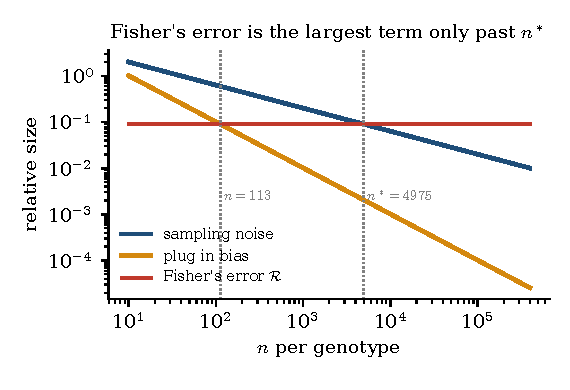
\includegraphics[width=0.62\textwidth]{figures/ftns_f4_errors.pdf}
\caption{Three sources of error in estimating $\Delta\wbar$ from a viability assay. Sampling noise
falls like $n^{-1/2}$, the plug in bias like $n^{-1}$, and Fisher's structural error not at all.
Below $n=113$ the estimator's own bias exceeds Fisher's; only past $n^\ast=4975$ does Fisher's
error become the largest term, and that is at $s=0.3$.}
\label{ftns:fig:errors}
\end{figure}

Read the last column. At every sample size a real experiment has used, the dominant term is
noise rather than either bias; below a hundred zygotes per genotype the estimator's own upward bias
exceeds Fisher's error; and Fisher's error becomes the largest term only past five thousand, at
$s=0.3$, which is not a realistic selection coefficient. This is a further reason nobody noticed.

\section{The delta method, and what it does not cover}
\label{ftns:sec:deltamethod}

The delta method is worth stating in full because its two outputs are exactly the two things being
confused.

Let $\hat\vartheta=\vartheta+\varepsilon$ with $\E\varepsilon=0$ and $\Var\varepsilon=\Sigma$, and let
$g$ be smooth. Expanding to second order and taking the variance uses the \emph{first} derivative
while taking the expectation uses the \emph{second}:
\[
\Var\big(g(\hat\vartheta)\big)\approx\nabla g^\top \Sigma\nabla g,
\qquad
\E\big[g(\hat\vartheta)\big]-g(\vartheta)\approx\tfrac12\operatorname{tr}\big(\nabla^2g\,\Sigma\big).
\]
For $g=\sA=2pq\alpha^2$ with $\alpha=c^\top\theta$, $c=(p,q-p,-q)$, one has $\nabla g=4pq\alpha\,c$
and $\nabla^2g=4pq\,cc^\top$, giving $\Var(\hat\sigma^2_A)\approx16p^2q^2\alpha^2\,c^\top\Sigma c$ and
bias $\approx2pq\,c^\top\Sigma c$, the two numbers of Section \ref{ftns:sec:bias}.

Now the point. Both $\R$ and the delta method bias are second order Taylor terms, they look alike,
and they are different objects. $\R$ is second order in a \emph{deterministic} expansion of
$\wbar(p)$ in $\Delta p$: the population moving. The delta method bias is second order in a
\emph{stochastic} expansion in $\hat\theta-\theta$: the sample not being the population. Compute a
delta method standard error, or bootstrap one, and the second is addressed while the first is
untouched. The ritual of uncertainty quantification is complete and the error survives it.

\section{Why the failure needs two or more loci}
\label{ftns:sec:twoloci}

Theorem \ref{ftns:thm:whole} says $\R=0$ when the motion is tangential to $\HW$. Whether the population
can move transversally is a question about which coordinates \emph{persist}.

At one locus with random mating and discrete generations, selection does push the adult genotype
proportions off Hardy Weinberg, but random mating restores them exactly among next generation's
zygotes. The transverse coordinate exists within a generation and is annihilated at the start of
the next: no memory, not a state variable, unable to accumulate. In continuous time with
Hardy Weinberg maintained, $\R\equiv0$ identically. So the entire persistent state is the vector
of allele frequencies, every direction of motion is tangential, and Fisher's claim is not
approximately right but right.

With two loci this changes qualitatively. Recombination does not set the linkage disequilibrium $D$
to zero in one generation; it multiplies it by roughly $(1-r)$. So $D$ is a genuine state variable
with its own dynamics and its own memory, selection can drive it, and epistasis means it carries
fitness. Section \ref{ftns:sec:exB} is the extreme case; Section \ref{ftns:sec:qle} the generic one.

The counting makes it stark. Under random mating the persistent state of an $L$ locus biallelic
system is the gamete frequency vector, a simplex of dimension $2^L-1$, of which exactly $L$
coordinates are allele frequencies.

\begin{center}
\begin{adjustbox}{max width=\textwidth}
\begin{tabular}{rrrr}
\toprule
loci $L$ & dimension of state & visible to $\sA$ & fraction visible \\
\midrule
$1$  & $1$ & $1$ & $100\%$ \\
$2$  & $3$ & $2$ & $66.7\%$ \\
$3$  & $7$ & $3$ & $42.9\%$ \\
$5$  & $31$ & $5$ & $16.1\%$ \\
$10$ & $1{,}023$ & $10$ & $0.98\%$ \\
$20$ & $1{,}048{,}575$ & $20$ & $0.0019\%$ \\
\bottomrule
\end{tabular}
\end{adjustbox}
\end{center}

\begin{quote}
The additive genetic variance tracks $L$ of the $2^L-1$ dimensions of the state. Fisher's assertion
is that the population never moves in the other $2^L-1-L$.
\end{quote}

At $L=1$ that assertion is a theorem. At $L=2$ it is a substantive and false claim about one third
of the state space being inert. At $L=20$ it is a claim about all but two thousandths of one
percent. This is why the one locus case is not a special case of the general one but its opposite,
and it is the sharpest form of the insistence that a one locus analysis cannot settle a
whole genome claim (Figure \ref{ftns:fig:dim}, left).

\begin{figure}[t]
\centering
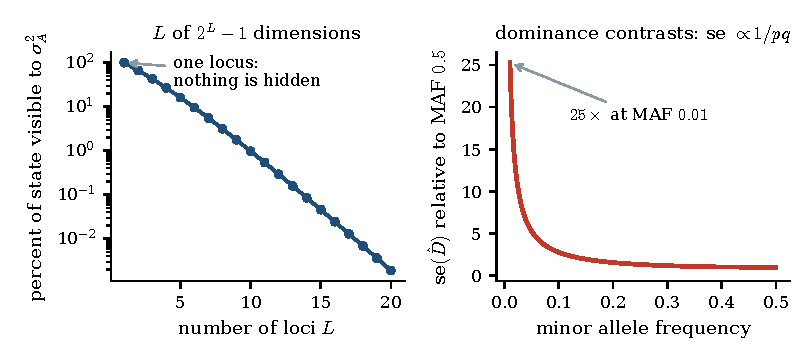
\includegraphics[width=\textwidth]{figures/ftns_f9_dim.pdf}
\caption{Left: the fraction of the persistent state that the additive genetic variance can see,
$L$ of $2^L-1$ dimensions. Right: dominance contrasts are strongly heteroskedastic, with
$\operatorname{se}(\hat D)\propto1/pq$, so the standard errors vary by a factor of twenty five
across the allele frequency spectrum. Any genome wide analysis must be built around per locus
standard errors.}
\label{ftns:fig:dim}
\end{figure}

\section{Sparsity is not a convenience}
\label{ftns:sec:sparsity}

The same counting explains why sparsity, which can look like a modelling fashion, is forced.

The additive model on $L$ biallelic loci has $L+1$ parameters. The saturated model on gametes has
$2^L$. So there are $2^L-L-1$ interaction parameters: about a billion at $L=30$, and beyond any
conceivable data by $L=60$. No experiment estimates them. No experiment ever will.

Some assumption restricting the interactions is therefore not optional; the problem is not well
posed without one. It cannot be a smoothness bound, since epistasis is not smooth in gene content. A magnitude bound, such as a dense variance component spreading a small effect over every interaction, does make the problem answerable, but only in aggregate: it estimates how large the interactions are in total and singles out none of them. If the interactions that matter are to be found, what remains is an assumption about how \emph{many} of them matter. That is sparsity, and it enters not because it is elegant but because it is the only class of assumption under which an exponentially overparameterized problem says which interactions matter. The two are combined in Section \ref{ftns:sec:stephens}.

Seen this way, Fisher and the horseshoe are doing the same thing and differ in one respect:

\begin{center}
\begin{adjustbox}{max width=\textwidth}
\begin{tabular}{lll}
\toprule
& Fisher (1930a, 1958) & global local shrinkage \\
\midrule
assumption & $\kappa_\ell=1$ for all $\ell$ & $\kappa_\ell\sim\text{Beta}(1/2,1/2)$ at $\tau=1$ \\
interactions retained & none & a data determined few \\
sparsity level & fixed at zero, a priori & estimated, as $\hat\tau$ \\
refutable & no & yes \\
\bottomrule
\end{tabular}
\end{adjustbox}
\end{center}

Fisher closed an exponentially overparameterized problem by fiat in 1930. That was reasonable
and, by Table \ref{ftns:tab:hs}, close to right; his mistake was to write the fiat as a theorem. The
modern move is the same instinct made falsifiable, and the number carrying the content is
$\hat\tau$, an estimate of how additive a genome is.

Sparsity also explains the one favourable result of Section \ref{ftns:sec:se}: because a few loci carry
almost the whole nonadditive total, estimating a few things well suffices for the aggregate, whose
relative error therefore falls like $L^{-1/2}$ even though no single locus is ever resolved.

\section{Why more parameters make it worse}
\label{ftns:sec:worse}

Five effects compound, and they push in the same direction.

\emph{The invisible subspace grows exponentially}: $L$ tangential coordinates against $2^L-1-L$
transverse ones.

\emph{Conjunctions of sharp nulls die}: Fisher's claim has posterior probability $\pi^L$, which at
$\pi=0.99$ and $L=10^4$ is $2.2\times10^{-44}$. Adding loci strictly hurts a universal claim,
however well each locus behaves.

\emph{Plug in bias in quadratic functionals scales with the parameter count}: the delta method bias
is $\tfrac12\operatorname{tr}(\nabla^2g\,\Sigma)$, a trace over the parameter space, so with $p$
parameters and $n$ observations it is $O(p/n)$ rather than $O(1/n)$. In the modern regime where $p$
is comparable to $n$ it does not vanish at all.

\emph{Selection on the estimate inflates it}: if loci are chosen for attention because
$\hat\delta_\ell$ was large, the retained values are biased upward. Shrinkage corrects this
automatically; plug in estimation does not.

\emph{The uncertainty quantification degrades exactly where it is needed}: Section \ref{ftns:sec:se}
found the nominal $95$ percent credible interval for $\sum_\ell\delta^2_\ell$ covering as little as
$60$ percent of the time.

\section{A prescription}
\label{ftns:sec:prescription}

What we would ask of a genomics study that uses any of this, ordered by how much difference each
makes.

\begin{enumerate}
\item \emph{Name the estimand.} State whether the reported quantity is $\sA$, the quantity
effect, or $d\mbar/dt$, the total. They are different numbers and the literature routinely uses the
language of the second while computing the first. The phrase \emph{rate of increase in fitness}
should not appear over a variance component.

\item \emph{Write $\kappa=1$ down as an assumption when you use it.} A study reporting $\sA$ and
concluding something about the change in mean fitness has assumed every nonadditive deviation in
the genome is exactly zero: a strong assumption, almost certainly false, belonging in the
assumptions rather than in the arithmetic.

\item \emph{Do not let a standard error stand in for a check on the formula.} By
Section \ref{ftns:sec:deltamethod} the delta method and the bootstrap quantify noise in the inputs and
are silent about $\R$. Report both, or state which has not been addressed.

\item \emph{Estimate the sparsity level and report it.} $\hat\tau$, or better the whole estimated
$G$, is the interesting number and is almost never reported. The choice is not between assuming all
interactions vanish and estimating all of them, neither being possible, but between fixing the
sparsity level and estimating it.

\item \emph{Use per locus standard errors.} Dominance contrasts have
$\operatorname{se}(\hat D)\propto1/pq$, a twenty five fold spread from minor allele frequency $0.5$
to $0.01$ (Figure \ref{ftns:fig:dim}, right). A homoskedastic analysis is not an approximation here, it
is a misspecification.

\item \emph{Use the correct functional.} $\sum_\ell(\E[\delta_\ell\mid y])^2$ is not the posterior
mean of $\sum_\ell\delta^2_\ell$, which requires the $\sum_\ell\Var(\delta_\ell\mid y)$ term.

\item \emph{Do not quote shrinkage credible intervals for quadratic functionals unchecked.} Report a
point estimate with a Monte Carlo or bootstrap standard error, and check any interval's coverage
by simulation.

\item \emph{Design across loci, not within them.} Detection at a single locus needs
$n\approx50\,s^{-4}$, which is unattainable, while information about the distribution of $\kappa$
accumulates in $L$. A genome wide design with modest per locus depth therefore beats a deep design
at few loci, which inverts the usual instinct.

\item \emph{Test the tangency, which is measurable.} Whether $\R$ is large is a question about
whether the association coordinates are moving, and those are observable: the Hardy Weinberg
disequilibrium coefficient in Lindley's parametrization and the linkage disequilibrium spectrum. A
study reporting both stationary has earned Fisher's assumption for its population. A study
reporting neither has assumed it.
\end{enumerate}

Item 9 is the one we would press hardest, because it converts a foundational dispute into an
empirical question. By Corollary \ref{ftns:thm:lindley} the constant genic environment condition is
exactly $\dot\alpha=0$, necessary as well as sufficient at a biallelic locus. Nobody need argue
about whether the Fundamental Theorem holds in general. One can look.

\chapterpart{Context, programme, and limits}

\section{Where this programme already lives}
\label{ftns:sec:lives}

Read alone, Part II sounds like a proposal to build something new. It is not. Almost every
component exists, most of it built by Matthew Stephens and Peter Carbonetto, and the lineage runs
back through Donnelly and Pritchard to the 1972 sampling formula.

Hoppe (1984) showed that the sampling formula arises from a P\'olya urn scheme, and Donnelly (1986) built on it: each new gene is
a novel allele with probability proportional to $\theta$, or a copy of an existing one with
probability proportional to its current count. That urn is the Chinese restaurant process and the
rule is the posterior predictive of a Dirichlet process. Donnelly and Tavar\'e (1986) worked out the
corresponding genealogical structure. So the Bayesian skeleton of Section \ref{ftns:sec:esf} was
articulated by a population geneticist a decade before the machine learning literature adopted the
same objects.

Fourteen years later, Pritchard, Stephens and Donnelly (2000) built STRUCTURE on Dirichlet priors
over allele frequencies and admixture proportions. Stephens and Donnelly (2000) gave importance
sampling for coalescent likelihoods; Stephens, Smith and Donnelly (2001) used an approximate
coalescent prior for haplotype reconstruction. None of this was framed as an argument about Bayes.
It was framed as population genetics, and the priors were the biology.

A last observation on the same theme. Li and Stephens (2003) introduced a hidden Markov copying
model in which each new haplotype is an imperfect mosaic of those already seen: an approximation to
the coalescent and, structurally, a prior over haplotypes, on which essentially every modern
imputation, phasing and local ancestry pipeline is built. Any contemporary genomic data set has
therefore had a prior applied before anyone sees the genotypes, and the prior does real work, since
it is what fills in the untyped variants. One may decline to be a Bayesian in one's own analysis;
one cannot decline the prior embedded in one's data.

\section{The empirical Bayes programme, and two corrections}
\label{ftns:sec:stephens}

The argument of Part II reduces to: do not fix the sparsity level, estimate it. That is the
organizing idea of Stephens's methodological work, executed more carefully than here.

\emph{Adaptive shrinkage} (Stephens, 2017) takes a vector of estimates with standard errors, posits
a unimodal prior $g$ on the underlying effects, estimates $g$ by nonparametric maximum likelihood,
and returns shrunken estimates and local false sign rates. The prior is not chosen at all; it is a
nonparametric object fitted to the data.

\emph{Multivariate adaptive shrinkage} (Urbut, Wang, Carbonetto and Stephens, 2019) extends this to
many conditions, learning the covariance structure of effects rather than assuming it. In the
present problem the analogue would be learning how nonadditive deviations covary across
environments or populations, which is a question nobody has asked of dominance deviations.

\emph{Variable selection} (Servin and Stephens, 2007; Carbonetto and Stephens, 2012) puts the
spike and slab into association analysis with the mixing weight estimated from data, and
\emph{SuSiE} (Wang, Sarkar, Carbonetto and Stephens, 2020) makes the fine mapping version tractable.

\subsection{Comparison with the horseshoe}

Both are normal scale mixtures; they differ in what they do with the mixing measure.

\begin{center}
\begin{tabularx}{\textwidth}{l>{\raggedright\arraybackslash}X>{\raggedright\arraybackslash}X}
\toprule
& horseshoe & adaptive shrinkage \\
\midrule
mixing measure & half Cauchy, fixed shape & unimodal, estimated by NPMLE \\
free parameters & one ($\tau$) & mixture weights on a scale grid \\
point mass at zero & impossible & available \\
noise variance & common & per observation $\operatorname{se}_\ell$ \\
computation & MCMC or EB search & convex, seconds \\
tails & Cauchy; never overshrinks & set by the largest grid scale \\
headline output & posterior mean & posterior mean and local false sign rate \\
\bottomrule
\end{tabularx}
\end{center}

\paragraph{Correction one.} For the estimand that matters, a functional of $G$, a nonparametric
estimate of $G$ is the better instrument. Our $\hat\tau$ is a one parameter summary of what adaptive
shrinkage estimates as a whole distribution, and heteroskedasticity settles the matter: dominance
contrasts have $\operatorname{se}\propto1/pq$, so per locus standard errors vary twenty five fold
across the allele frequency spectrum, and the horseshoe as used here has no place to put them.

\paragraph{Correction two.} Zhou, Carbonetto and Stephens (2013) introduced the Bayesian sparse
linear mixed model, combining a sparse spike and slab component with a dense polygenic one. For
this problem that is probably the right model class and a pure sparsity prior is not. The biology
suggests two contributions: dominance deviations at ordinary segregating loci, numerous and
individually tiny, since inbreeding depression testifies to directional dominance almost everywhere
and Section \ref{ftns:sec:undetected} put their whole genome contribution at about a tenth of a percent
spread thin; and epistatic contributions, which by Section \ref{ftns:sec:qle} are not damped by
recombination and are plausibly concentrated. That is a dense background plus a sparse foreground.
We would now propose the two component model, and expect the dense component to absorb the
dominance and the sparse component to carry the epistasis. That is a testable prediction.

\paragraph{Where the horseshoe wins.} Tail robustness. Because the mixing measure has genuinely
Cauchy tails, a large signal is never overshrunk: $0.94$ retained at six standard deviations and
$0.967$ at eight, identical across $\tau$. A finite scale grid inherits whatever tail its largest
component provides.

\paragraph{An awkwardness worth naming.} Fisher's hypothesis is a point mass at $\kappa=1$, and the
horseshoe is continuous, so $\Prob(\delta=0)=0$: it cannot represent the hypothesis being tested.
That is why Section \ref{ftns:sec:jeffreys} used a spike and slab and Section \ref{ftns:sec:horseshoe} a
horseshoe. Adaptive shrinkage and spike and slab variable selection both carry a point mass and
would allow a single model throughout.

\section{Computation at genome scale}
\label{ftns:sec:compute}

A natural objection is that whole genome matrices are of order $10^5\times10^5$ and too large to
handle. Four points, in increasing order of importance.

\paragraph{Even brute force is not blocked.} A dense Cholesky costs $p^3/3$ flops, or
$3.3\times10^{14}$ at $p=10^5$. Timing factorizations at $p=2000$ to $8000$ on an ordinary machine
sustaining $23$ GFLOP/s and extrapolating gives four hours; on one CPU node at a teraflop, six
minutes; on a single GPU in double precision, under a minute. Dense storage is $80$ GB.

\paragraph{The relevant dimension is $\min(n,p)$.} The whole genome least squares system involves
$(X^\top X+\lambda I)$ of order $p$, but by the Woodbury identity every quantity needed is
obtainable from $(XX^\top+\lambda I)$ of order $n$, the number of individuals: the genomic
relationship matrix of VanRaden (2008), standard equipment in animal breeding, and the matrix whose single eigendecomposition makes the exact mixed model association tests of Zhou and Stephens (2012) fast. With ten thousand
individuals and a hundred thousand markers one factorizes a $10^4\times10^4$ matrix, costing $0.3$
TFLOP.

\paragraph{One never forms any matrix.} Iterative methods need only the action of $X$ and $X^\top$
on a vector, and variance components follow by combining this with stochastic trace estimation,
which is how biobank scale mixed models are fitted. Analyses with half a million individuals and a
million markers are routine, so $10^5\times10^5$ is well behind the frontier.

\paragraph{For the horseshoe specifically.} The one expensive step is sampling a $p$ dimensional
Gaussian with dense covariance, naively $O(p^3)$. Bhattacharya, Chakraborty and Mallick (2016) give
an \emph{exact} algorithm costing $O(n^2p)$, a hundredfold saving at $n=10^4$, $p=10^5$. Johndrow,
Orenstein and Bhattacharya (2020) push global local MCMC to $p$ in the hundreds of thousands to
millions, and Carbonetto and Stephens (2012) give a variational route. The sparsity is itself a
computational resource: most coordinates have $\kappa_\ell$ near one and can be screened out at
each sweep.

\section{The omnigenic model, and the serious threat to sparsity}
\label{ftns:sec:omnigenic}

Boyle, Li and Pritchard (2017) argue that for complex traits the effects are not sparse at all:
because regulatory networks are densely interconnected, essentially every expressed gene
contributes, and most heritability lies outside the loci of largest effect. If that view is correct
for nonadditive deviations as well as additive ones, the sparsity assumption underlying Part II is
wrong.

The consequences are not what one might expect. If the truth is dense and each deviation is small against its standard error, a horseshoe shrinks many genuinely nonzero deviations toward zero and the estimate of $\sum_\ell\delta_\ell^2$ becomes badly conservative. In a simulation with all of $2000$ deviations nonzero and normal with standard deviation half a standard error, the fitted $\hat\tau$ is $0.03$ and the posterior total recovers $30$ percent of the true one; at two standard errors $\hat\tau$ is $1.2$ and it recovers $97$ percent, which is the graceful degradation of Section \ref{ftns:sec:horseshoe}. The omnigenic threat is the first case, many small deviations. So the omnigenic view, if right, does not rescue Fisher: it makes the nonadditive
total \emph{larger} than the simulations here suggest while invalidating the instrument used to
measure it. The conclusion strengthens and the method fails, and the response is the two component
model of Section \ref{ftns:sec:stephens}.

One qualification runs in Fisher's favour. The omnigenic argument concerns effects on phenotype
propagating through regulatory networks. The quantity at issue in the Fundamental Theorem is the
departure of \emph{fitness} from additivity in gene content, a different functional that need not
inherit the density of the underlying trait architecture. Whether it does is an open empirical
question and, so far as we can find, an unasked one.

\section{A thread through the whole story}
\label{ftns:sec:cedric}

One further connection deserves recording, because it ties the deterministic and stochastic halves
of this chapter to a single person.

Cedric A. B. Smith of the Galton Laboratory is the Smith of Mulholland and Smith (1959), the
inequality that gives the one locus monotonicity theorem which Section \ref{ftns:sec:undetected}
identifies as the decoy for the Fundamental Theorem. He is also the Smith of Haldane and Smith
(1947), on linkage between haemophilia and colour blindness, among the first Bayesian analyses in
human genetics. And he is the Smith of Smith and Stephens (1995), on estimating multipoint
recombination fractions, and Smith and Stephens (1996) on linkage heterogeneity, with D. A.
Stephens at Imperial College: the Bayesian treatment of the recombination fraction, sixty three
years after Haldane put a spike on it.

One line therefore runs from Haldane's 1932 prior on $\rho$, through Haldane and Smith in 1947 and
Mulholland and Smith in 1959, who supply the true theorem mistaken for Fisher's, to Smith and
Stephens in the 1990s, estimating the decay rate of the transverse coordinate whose motion is $\R$. The
obstruction and the apparatus for measuring it were built by overlapping people in overlapping
decades and never connected.

\section{A research programme}
\label{ftns:sec:programme}

Concretely, and in the order we would do it.

\begin{enumerate}
\item Compute per locus dominance contrasts and standard errors from a genotyped panel with a
fitness proxy, standardized so that noise is unit normal, retaining the per locus standard errors $\operatorname{se}_\ell$.
\item Fit adaptive shrinkage to estimate the distribution $G$ of the deviations nonparametrically,
and report $G$ rather than a single $\hat\tau$.
\item Fit the two component sparse plus polygenic model to separate the dense dominance background
from any concentrated epistatic signal, testing the prediction of Section \ref{ftns:sec:stephens}.
\item Report $\sum_\ell\delta^2_\ell$ as the posterior mean of the correct functional, with a
Monte Carlo standard error.
\item Separately, and independently of all the above, measure the tangency directly: Lindley's
Hardy Weinberg disequilibrium coefficient and the linkage disequilibrium spectrum, and whether
either moves on the timescale of selection.
\item Derive \eqref{ftns:eq:qle} analytically, and settle the asymmetric case that the numerics left
open.
\end{enumerate}

Item 5 is the one to do first if only one can be done.

\section{What would change our mind}
\label{ftns:sec:mind}

Since this chapter asks the reader to accept a statistical supplement to a mathematical result, it is
only fair to say what would make the supplement worthless.

If real genomic panels gave $\hat\tau$ so small that the posterior for $\sum_\ell\delta_\ell^2$
concentrated near zero, Fisher's $\kappa=1$ would be an excellent genome wide approximation and
Part II an elaborate way of confirming him. Apart from the dense check of Section \ref{ftns:sec:omnigenic}, our simulations assume sparsity between one and ten
percent, and nothing establishes that real genomes lie there.

Conversely, if the association coordinates were shown to be stationary in real populations, so that
Lindley's coefficient and the linkage disequilibrium spectrum do not move on the timescale of
selection, then $\R$ would be small for empirical rather than assumed reasons, and the constant
genic environment would be an observation rather than a tautology. That would not rescue the
theorem, which would remain false, but it would make the falsehood harmless.

Both are measurements and neither has been made.

\section{Conclusion}

Fisher stated a falsehood, and the deterministic argument establishing it is unconditional: no
prior, no sampling model, no sparsity assumption, true of every population and every genome.
Nothing here disturbs it. What we have tried to add is an account of four things it does not reach.

\emph{What the error is.} Lemma \ref{ftns:lem:moving} and Theorem \ref{ftns:thm:whole} identify it as the
transverse component of a motion, with the additive genetic variance registering exactly the
tangential part. Fisher's assertion is that a population never departs from Hardy Weinberg
proportions and linkage equilibrium, and his 1941 constant genic environment condition is the
statement that Lindley's disequilibrium coefficient is stationary, which
Corollary \ref{ftns:thm:lindley} shows to be necessary and sufficient at a biallelic locus.

\emph{How much it matters.} At one locus, for the shape of Example~\ref{ftns:ex:A}, the relative error is $0.28\,s$ and vanishes as selection
weakens; between loci it is $\epsilon\sqrt{p_Aq_Ap_Bq_B}$ and does not, and is not damped by
recombination. So Fisher's error is negligible in the direction that can be bounded and unbounded
in the direction that cannot.

\emph{Why the correction did not take.} Because $n^\ast\approx50\,s^{-4}$; because the theorem is
exactly true in the setting where it is taught; because the proposition everyone tests is a
different and true one; because the neglected term has never been computable; and because at
experimental sample sizes Fisher's error is not even the largest error present.

\emph{What survives.} $\kappa=1$ is a prior, and a good one: the posterior mean of $\kappa$ across
loci runs from $0.86$ to $0.98$, so Fisher is right at almost every locus. He is wrong in
aggregate, by the entire quantity, and the aggregate error is carried by a small minority of loci.
The replacement is not a different theorem but an estimated sparsity level, and the object to
report is the distribution of $\kappa$ rather than a point mass at its endpoint.

The epitaph we would propose is that Fisher had an excellent prior and a bad theorem. The theorem
should go. The prior deserves to survive, under that name, with the error bars this chapter has tried
to supply, and with the one measurement that would settle the matter still to be made.



\section{Proofs and supplementary derivations}
\label{ftns:app:proofs}

\paragraph{Equivalence of the three forms of the remainder.} Since $\sum_{u,v}P_{uv}\delta_{uv}=0$, mean fitness may be written against either the fitted vector
or the original: $\mbar=\sum_{u,v}P_{uv}A_{uv}=\sum_{u,v}P_{uv}m_{uv}$. Differentiating the first
gives $\sA+2\sum_up_u\dot\beta_u$; differentiating the second and splitting $m=A+\delta$ afterwards
gives $\sA+\sum_{u,v}\dot P_{uv}\delta_{uv}$. The first terms agree by Lemma \ref{ftns:lem:moving}, so
\[
2\sum_u p_u\dot\beta_u \;=\; \sum_{u,v}\dot P_{uv}\delta_{uv}
\;=\; \sum_{u,v}p_up_v\delta_{uv}\frac{d}{dt}\Big(\frac{P_{uv}}{p_up_v}\Big),
\]
the last being Kimura's form, whose equality with the first was proved by Lessard (1997).

\paragraph{The Beta$(\tfrac12,\tfrac12)$ law of the shrinkage weight.} If $\lambda\sim C^+(0,1)$ then $\lambda^2$ has density proportional to $x^{-1/2}(1+x)^{-1}$, a
Beta prime$(\tfrac12,\tfrac12)$ law. The map $x\mapsto x/(1+x)$ carries Beta prime$(a,b)$ to
Beta$(a,b)$, so with $\tau=1$ we have $1-\kappa=\lambda^2/(1+\lambda^2)\sim
\text{Beta}(\tfrac12,\tfrac12)$ and hence $\kappa\sim\text{Beta}(\tfrac12,\tfrac12)$ by symmetry.
For general $\tau$ the induced density is
\[
p(\kappa\mid\tau)\;\propto\;\frac{\kappa^{-1/2}(1-\kappa)^{-1/2}}{1-(1-\tau^2)\kappa},
\qquad
p(\kappa\mid y,\tau)\;\propto\;\frac{e^{-\kappa y^2/2}(1-\kappa)^{-1/2}}{1-(1-\tau^2)\kappa}.
\]

\paragraph{Heteroskedasticity of the dominance contrast.} Under Hardy Weinberg with $N$ genotyped individuals, $n_{11}=Np^2$, $n_{12}=2Npq$, $n_{22}=Nq^2$,
so
\[
\Var(\hat D)=\sigma^2\Big(\frac{1}{n_{11}}+\frac{4}{n_{12}}+\frac{1}{n_{22}}\Big)
=\frac{\sigma^2}{N}\Big(\frac1p+\frac1q\Big)^2=\frac{\sigma^2}{N(pq)^2},
\]
so $\operatorname{se}(\hat D)\propto 1/pq$. From minor allele frequency $0.5$ to $0.01$ this is a
factor of $25.3$. Simulation confirms the analytic form to within two percent across that range.

\section{Numerical verification}
\label{ftns:app:num}

Every quantity reported in this chapter was recomputed independently. The following checks were made.

\begin{center}
\begin{tabularx}{\textwidth}{l>{\raggedright\arraybackslash}X>{\raggedright\arraybackslash}X}
\toprule
Claim & Check & Result \\
\midrule
Lemma \ref{ftns:lem:moving} & random non HW $P$, $k=2,3,4$ & max error $3.6\times10^{-15}$ \\
Theorem \ref{ftns:thm:whole} & random $P$ on full simplex, $L=1,2,3$ & max error $6.2\times10^{-15}$ \\
vanishing criterion & $\partial_t\log P\in V$ imposed & $|\R|<1.8\times10^{-15}$ \\
Theorem \ref{ftns:thm:main} & random $W$, $k=2,\dots,10$, $2000$ draws & max error $1.6\times10^{-15}$ \\
three forms of $\R$ agree & random smooth path, $k=4$ & agree to $10$ significant figures \\
Example \ref{ftns:ex:A} & all six quantities & exact to six decimals \\
Example B trajectory & four generations & exact to six decimals \\
$\kappa\sim\text{Beta}(\tfrac12,\tfrac12)$ & $4\times10^5$ draws, five quantiles & max deviation $0.0014$ \\
$D^\ast=\epsilon p_Aq_Ap_Bq_B/r$ & $r=0.5,0.25$; $\epsilon\in[0.005,0.02]$ & within $0.5\%$ \\
$|\R|/(\sA/\wbar)=\epsilon\sqrt{p_Aq_Ap_Bq_B}$ & grid in $s,\epsilon,r$ & ratio in $[0.224,0.255]$ \\
$\E[K_n]=\sum\theta/(\theta+i)$ & CRP simulation, $n=100$, $\theta=5$ & $15.76$ vs $15.72$ \\
ESF conditional free of $\theta$ & $n=8$, $K=3$, three $\theta$ & identical to six figures \\
\bottomrule
\end{tabularx}
\end{center}

\begin{center}
\begin{tabularx}{\textwidth}{l>{\raggedright\arraybackslash}X>{\raggedright\arraybackslash}X}
\toprule
Claim & Check & Result \\
\midrule
delta method s.e.\ of $\hat\sigma^2_A$ & $4000$ replicates at five $n$ & within $5\%$ \\
plug in bias $10.19/n$ & exact, as $\hat\alpha$ is unbiased; $20{,}000$ replicates at $n=25,50,100$ & within $3.4\%$, under $1.4$ Monte Carlo s.e. \\
$\operatorname{se}(\hat D)\propto1/pq$ & five allele frequencies & within $2\%$ \\
Theorem \ref{ftns:thm:expfam}, main effects & random families with $4$, $8$ and $16$ genotypes & $|\langle\delta,\partial\log P/\partial c\rangle_t|<10^{-15}$ \\
Theorem \ref{ftns:thm:expfam}, factorization & random families and velocities & relative error $<5\times10^{-7}$ \\
$\R=D\,\mathcal{I}(\alpha)\,\dot\alpha$ & $200$ random states and velocities & relative error $<7\times10^{-8}$ \\
Lemma \ref{ftns:lem:info} & numerical information matrix in $(p,\alpha)$ & off diagonal $<10^{-10}$ \\
Examples \ref{ftns:ex:ls} to \ref{ftns:ex:lindleynum} & normal equations, three velocities, three forms of $\R$ & agree to six decimals \\
Example \ref{ftns:ex:twolocus} & weighted regression and Proposition \ref{ftns:prop:twolocus} & exact \\
Corollary \ref{ftns:cor:relerr} & Example \ref{ftns:ex:A} and four values of $s$ & exact \\
Example \ref{ftns:ex:assay} & grid quadrature, reproduces Table \ref{ftns:tab:bf} entries & to the printed figures \\
retained fractions & quadrature against $2\times10^6$ Monte Carlo draws & three decimals \\
\bottomrule
\end{tabularx}
\end{center}

Two computational notes. The Bayes factors of Table \ref{ftns:tab:bf} were first obtained by adaptive
two dimensional quadrature, which proved unreliable in the tails; the reported values come from a
windowed grid centred on the posterior mode with the integrand evaluated on the log scale. The
horseshoe computations of Section \ref{ftns:sec:horseshoe} use the exact conditional
\eqref{ftns:eq:kappapost} on a grid in $u=\sqrt{1-\kappa}$, with $\tau$ fitted by bounded one
dimensional maximization of the marginal likelihood, and report $\sum_\ell\E[\delta^2_\ell\mid y]$
rather than squared posterior means, for the reason given in Section \ref{ftns:sec:se}. The retained fraction and threshold tables of that section, Table \ref{ftns:tab:hs} and the genome size table
were checked by quadrature and by direct Monte Carlo over the half Cauchy prior: the entries printed
are the ones \eqref{ftns:eq:kappapost} implies.

\section{Notation}
\label{ftns:app:notation}

\begin{center}
\begin{adjustbox}{max width=\textwidth}
\begin{tabular}{ll}
\toprule
Symbol & Meaning \\
\midrule
$P_{uv}(t)$, $P_g(t)$ & genotype frequencies, one locus and whole genome \\
$p_u$, $p_{ij}$ & allele frequencies \\
$m_{uv}$, $w_{ij}$ & Malthusian parameters; Wrightian fitnesses \\
$\mbar$, $\wbar$ & mean Malthusian parameter; mean fitness \\
$V$ & subspace of arrays additive in gene content \\
$\Pi_t$ & orthogonal projection onto $V$ in $L^2(P_t)$ \\
$\beta_u$, $\alpha_i$ & average effects (Ewens's and the centred parametrization) \\
$\alpha$, $\mathcal{I}(\alpha)$ & Lindley's coefficient; its Fisher information \\
$\alpha$ & average effect of a substitution in the viability assay \\
$A=\Pi_tm$ & breeding value; the fitted vector \\
$\delta=m-A$ & nonadditive deviation; the residual \\
$\sA$ & additive genetic variance \\
$\R$ & the remainder, $\sum_{u,v}\dot P_{uv}\delta_{uv}=d\mbar/dt-2\sum_u\dot p_u\beta_u$ \\
$\HW$ & manifold of gene frequency product measures \\
$s$, $\epsilon$ & selection coefficient; epistatic coefficient \\
$D$ (one locus) & fitness curvature, $m_{11}-2m_{12}+m_{22}$ \\
$D$, $D_{AB}$, $D^\ast$ & two loci: linkage disequilibrium; its quasi equilibrium value \\
$\kappa_\ell$ & shrinkage weight at locus $\ell$ \\
$\tau$, $\lambda_\ell$ & global and local scales \\
$K$ & Jeffreys's Bayes factor for the null \\
$n^\ast$ & sample size at which $\R$ exceeds the sampling noise \\
$L$ & number of loci \\
\bottomrule
\end{tabular}
\end{adjustbox}
\end{center}

\section{Exercises}
\label{ftns:sec:exercises}

\begin{enumerate}[label=\arabic*.,leftmargin=*]
\item Under Hardy Weinberg proportions and $m=(\mu+a,\mu+d,\mu-a)$, solve the normal equations
\eqref{ftns:eq:normal2} and show that the average effect of a substitution is
$\beta_1-\beta_2=a+d(q-p)$ and that $\sA=2pq\{a+d(q-p)\}^2$.

\emph{Hint.} Under Hardy Weinberg the system is the regression of genotypic value on gene count;
subtract the two equations.

\item Show that under pure viability selection, $\dot P_{uv}=P_{uv}(m_{uv}-\mbar)$, one has
$d\mbar/dt=\sigma^2_G$, $2\sum_u\dot p_u\beta_u=\sA$ and $\R=\sigma^2_D$, for arbitrary genotype
frequencies and any number of alleles.

\emph{Hint.} Each term is a covariance under $P$ of $m$ with $m$, $A$ or $\delta$; use
$\delta\perp V$.

\item Prove Lemma \ref{ftns:lem:info} a second way, by computing the asymptotic variance of the plug
in estimate $\hat\alpha$ with the delta method. Evaluate $\mathcal{I}(\alpha)$ at
$P=(0.25,0.50,0.25)$.

\emph{Hint.} For a log contrast $\sum_gc_g\log\hat P_g$ with $\sum_gc_g=0$ the multinomial delta
method gives $n^{-1}\sum_gc_g^2/P_g$. The value is $1/16$.

\item Take $P=(0.20,0.40,0.40)$ and $m=(0,\,0.1,\,-0.1)$. Compute $\beta$ and $\delta$ from
\eqref{ftns:eq:normal2}, then confirm Proposition \ref{ftns:prop:resid}: $\sigma^2_D=D^2\mathcal{I}(\alpha)$.

\emph{Hint.} $D=-0.3$ and $1/\mathcal{I}(\alpha)=5+10+2.5=17.5$, so $\sigma^2_D=0.09/17.5=0.005143$;
the residuals are $(-0.0857,\,0.0857,\,-0.0429)$.

\item Prove the recombination formula $\R=-rD_{AB}E$ of Proposition \ref{ftns:prop:twolocus}. In
Example \ref{ftns:ex:twolocus}, find the recombination rate at which selection and recombination
together leave mean fitness momentarily constant.

\emph{Hint.} Recombination moves no allele frequency, so the whole change is remainder. The rate is
$r=0.0176/(D_{AB}E)=0.352$.

\item Show from Corollary \ref{ftns:cor:relerr} that at a biallelic locus
$|\R|/(\sA/\wbar)\le|D|/(8\wbar)$, with equality exactly at $p=\tfrac12$. Explain why the bound does
not depend on how strong the additive selection is.

\emph{Hint.} $pq\le\tfrac14$; the average excess cancels from the ratio.

\item In the exclusive or system of Section \ref{ftns:sec:exB}, verify by hand that
$\wbar=1.089$ at $x=(0.05,0.45,0.45,0.05)$, and show without computing any regression that every
average effect is zero.

\emph{Hint.} Mean fitness is $0.6+0.6\,\Prob(\text{the loci disagree})$, and the disagreeing
genotypes are $AaBb$, $AAbb$ and $aaBB$. For the second part use the symmetry $\sigma$.

\item Under the null, Table \ref{ftns:tab:bf} grows like $K\approx0.67\sqrt n$. How many zygotes
per genotype give $K=100$ at one locus? How many give posterior probability one half to the
conjunction of the null at $L=100$ independent loci, from equal prior odds?

\emph{Hint.} $(100/0.67)^2\approx2.2\times10^4$; for the conjunction, $\pi^L\approx e^{-L/K}$ and one
needs $K\ge L/\log2$, so $n\approx4.6\times10^4$.

\item Derive the closed form Bayes factor for Hardy Weinberg proportions in Example \ref{ftns:ex:mn}.
Evaluate it for counts $(25,50,25)$ and $(35,30,35)$.

\emph{Hint.} The Hardy Weinberg likelihood is $2^{n_{12}}p^{2n_{11}+n_{12}}q^{n_{12}+2n_{22}}$.
The values are $K=4.1$ and $K=1.0\times10^{-3}$.

\item At $\tau=1$ show that \eqref{ftns:eq:kappapost} is
$p(\kappa\mid y)\propto e^{-\kappa y^2/2}(1-\kappa)^{-1/2}$, that $\E[\kappa\mid y=0]=2/3$, and that
$\E[\kappa\mid y]\approx2/y^2$ for large $|y|$. Compare with the entries for $y=6$ in
Example \ref{ftns:ex:panel}.

\emph{Hint.} For large $|y|$ the mass sits near $\kappa=0$, where the posterior is approximately
exponential with rate $y^2/2$. At $y=6$ the approximation gives $0.056$ against $0.057$.

\item Show that $\sum_\ell(\E[\delta_\ell\mid y])^2\le\sum_\ell\E[\delta^2_\ell\mid y]$, and explain
why the gap is largest for loci whose contrasts lie near the shrinkage threshold.

\emph{Hint.} The gap is $\sum_\ell\Var(\delta_\ell\mid y)$; near the threshold the posterior for
$\kappa$ is spread over both prongs.

\item For the Ewens sampling formula show that $K_n$ is sufficient for $\theta$, and compute the
maximum likelihood estimate from $n=100$ genes carrying $k=15$ distinct alleles.

\emph{Hint.} The $\theta$ dependence is $\theta^{K_n}/\theta_{(n)}$; solve
$\sum_{i=0}^{99}\theta/(\theta+i)=15$ numerically, giving $\hat\theta=4.66$.
\end{enumerate}

\section*{References}

\begin{itemize}\itemsep2pt \small
\item Amari, S. (1985). \emph{Differential Geometrical Methods in Statistics}. Lecture Notes in
Statistics 28, Springer, New York.
\item Antoniak, C. E. (1974). Mixtures of Dirichlet processes with applications to Bayesian
nonparametric problems. \emph{Annals of Statistics} 2, 1152 to 1174.
\item Armagan, A., Dunson, D. B. and Clyde, M. (2011). Generalized beta mixtures of Gaussians.
\emph{Advances in Neural Information Processing Systems} 24, 523 to 531.
\item Bhattacharya, A., Chakraborty, A. and Mallick, B. K. (2016). Fast sampling with Gaussian
scale mixture priors in high dimensional regression. \emph{Biometrika} 103, 985 to 991.
\item Boyle, E. A., Li, Y. I. and Pritchard, J. K. (2017). An expanded view of complex traits: from
polygenic to omnigenic. \emph{Cell} 169, 1177 to 1186.
\item Carbonetto, P. and Stephens, M. (2012). Scalable variational inference for Bayesian variable
selection in regression, and its accuracy in genetic association studies.
\emph{Bayesian Analysis} 7, 73 to 108.
\item Carvalho, C. M., Polson, N. G. and Scott, J. G. (2010). The horseshoe estimator for sparse
signals. \emph{Biometrika} 97, 465 to 480.
\item Castilloux, A.-M. and Lessard, S. (1995). The fundamental theorem of natural selection in
Ewens' sense (case of many loci). \emph{Theoretical Population Biology} 48, 306 to 315.
\item Churchill, G. A. and Doerge, R. W. (1994). Empirical threshold values for quantitative trait
mapping. \emph{Genetics} 138, 963 to 971.
\item Crow, J. F. (1987). Population genetics history: a personal view. \emph{Annual Review of
Genetics} 21, 1 to 22.
\item Donnelly, P. (1986). Partition structures, P\'olya urns, the Ewens sampling formula, and the
ages of alleles. \emph{Theoretical Population Biology} 30, 271 to 288.
\item Donnelly, P. and Tavar\'e, S. (1986). The ages of alleles and a coalescent.
\emph{Advances in Applied Probability} 18, 1 to 19.
\item Edwards, A. W. F. (2002). The fundamental theorem of natural selection.
\emph{Theoretical Population Biology} 61, 335 to 337.
\item Egozcue, J. J., Pawlowsky Glahn, V., Mateu Figueras, G. and Barcel\'o Vidal, C. (2003).
Isometric logratio transformations for compositional data analysis. \emph{Mathematical Geology} 35,
279 to 300.
\item Etz, A. and Wagenmakers, E.-J. (2017). J. B. S. Haldane's contribution to the Bayes factor
hypothesis test. \emph{Statistical Science} 32(2), 313 to 329.
\item Ewens, W. J. (1972). The sampling theory of selectively neutral alleles.
\emph{Theoretical Population Biology} 3, 87 to 112.
\item Ewens, W. J. (1989). An interpretation and proof of the fundamental theorem of natural
selection. \emph{Theoretical Population Biology} 36, 167 to 180.
\item Ewens, W. J. (1992). An optimizing principle of natural selection in evolutionary population
genetics. \emph{Theoretical Population Biology} 42, 333 to 346.
\item Ewens, W. J. (2004). \emph{Mathematical Population Genetics}. Springer, New York.
\item Ewens, W. J. (2024). The fundamental theorem of natural selection: the end of a story.
\emph{Evolution} 78, 803 to 808.
\item Ferguson, T. S. (1973). A Bayesian analysis of some nonparametric problems.
\emph{Annals of Statistics} 1, 209 to 230.
\item Fisher, I. (1922). \emph{The Making of Index Numbers}. Houghton Mifflin, Boston.
\item Fisher, R. A. (1918). The correlation between relatives on the supposition of Mendelian
inheritance. \emph{Transactions of the Royal Society of Edinburgh} 52, 399 to 433.
\item Fisher, R. A. (1930a). \emph{The Genetical Theory of Natural Selection}. Oxford University
Press, Oxford.
\item Fisher, R. A. (1930b). Inverse probability. \emph{Proceedings of the Cambridge Philosophical
Society} 26, 528 to 535.
\item Fisher, R. A. (1932). Inverse probability and the use of likelihood. \emph{Mathematical
Proceedings of the Cambridge Philosophical Society} 28(3), 257 to 261.
\item Fisher, R. A. (1941). Average excess and average effect of a gene substitution.
\emph{Annals of Eugenics} 11, 53 to 63.
\item Fisher, R. A. (1958). \emph{The Genetical Theory of Natural Selection}, 2nd revised ed.
Dover, New York.
\item Haldane, J. B. S. (1932). A note on inverse probability. \emph{Mathematical Proceedings of
the Cambridge Philosophical Society} 28(1), 55 to 61.
\item Haldane, J. B. S. and Smith, C. A. B. (1947). A new estimate of the linkage between the genes
for colour blindness and haemophilia in man. \emph{Annals of Eugenics} 14, 10 to 31.
\item Hartl, D. L. and Clark, A. G. (2007). \emph{Principles of Population Genetics}, 4th ed.
Sinauer, Sunderland, Massachusetts.
\item Hoppe, F. M. (1984). P\'olya like urns and the Ewens' sampling formula. \emph{Journal of Mathematical Biology} 20, 91 to 94.
\item James, W. and Stein, C. (1961). Estimation with quadratic loss. In \emph{Proceedings of the
Fourth Berkeley Symposium}, Vol.\ 1, 361 to 379. University of California Press, Berkeley.
\item Jefferys, W. H. and Berger, J. O. (1992). Ockham's razor and Bayesian analysis.
\emph{American Scientist} 80, 64 to 72.
\item Jeffreys, H. (1935). Some tests of significance, treated by the theory of probability.
\emph{Proceedings of the Cambridge Philosophical Society} 31, 203 to 222.
\item Jeffreys, H. (1936). Further significance tests. \emph{Mathematical Proceedings of the
Cambridge Philosophical Society} 32, 416 to 445.
\item Jeffreys, H. (1961). \emph{Theory of Probability}, 3rd ed. Clarendon Press, Oxford.
\item Johndrow, J., Orenstein, P. and Bhattacharya, A. (2020). Scalable approximate MCMC algorithms for the
horseshoe prior. \emph{Journal of Machine Learning Research} 21, 1 to 61.
\item Kimura, M. (1958). On the change of population fitness by natural selection.
\emph{Heredity} 12, 145 to 167.
\item Kingman, J. F. C. (1961). A mathematical problem in population genetics.
\emph{Proceedings of the Cambridge Philosophical Society} 57, 574 to 582.
\item Kingman, J. F. C. (1975). Random discrete distributions. \emph{Journal of the Royal
Statistical Society B} 37, 1 to 22.
\item Kingman, J. F. C. (1978). The representation of partition structures.
\emph{Journal of the London Mathematical Society} 18, 374 to 380.
\item Kojima, K. and Kelleher, T. M. (1961). Changes of mean fitness in random mating populations
when epistasis and linkage are present. \emph{Genetics} 46, 527 to 540.
\item Lee, J. J. and Chow, C. C. (2013). The causal meaning of Fisher's average effect.
\emph{Genetics Research} 95, 89 to 109.
\item Lessard, S. (1997). Fisher's fundamental theorem of natural selection revisited.
\emph{Theoretical Population Biology} 52, 119 to 136.
\item Lessard, S. and Castilloux, A.-M. (1995). The fundamental theorem of natural selection in
Ewens' sense (case of fertility selection). \emph{Genetics} 141, 733 to 742.
\item Lessard, S. and Ewens, W. J. (2019). The left hand side of the fundamental theorem of natural
selection: a reply. \emph{Journal of Theoretical Biology} 472, 77 to 83.
\item Li, N. and Stephens, M. (2003). Modeling linkage disequilibrium and identifying recombination
hotspots using single nucleotide polymorphism data. \emph{Genetics} 165, 2213 to 2233.
\item Lindley, D. V. (1957). A statistical paradox. \emph{Biometrika} 44, 187 to 192.
\item Lindley, D. V. (1988). Statistical inference concerning Hardy Weinberg equilibrium. In
J. M. Bernardo, M. H. DeGroot, D. V. Lindley and A. F. M. Smith (eds), \emph{Bayesian Statistics
3}, 307 to 326. Oxford University Press, Oxford.
\item Ly, A., Verhagen, J. and Wagenmakers, E.-J. (2016). Harold Jeffreys's default Bayes factor
hypothesis tests. \emph{Journal of Mathematical Psychology} 72, 19 to 32.
\item MacKay, D. J. C. (1992). Bayesian interpolation. \emph{Neural Computation} 4, 415 to 447.
\item MacKay, D. J. C. (2003). \emph{Information Theory, Inference, and Learning Algorithms}.
Cambridge University Press, Cambridge.
\item Moran, P. A. P. (1964). On the nonexistence of adaptive topographies.
\emph{Annals of Human Genetics} 27, 383 to 393.
\item Morton, N. E. (1955). Sequential tests for the detection of linkage.
\emph{American Journal of Human Genetics} 7(3), 277 to 318.
\item Mulholland, H. P. and Smith, C. A. B. (1959). An inequality arising in genetical theory.
\emph{American Mathematical Monthly} 66, 673 to 683.
\item Price, G. R. (1972). Fisher's ``fundamental theorem'' made clear.
\emph{Annals of Human Genetics} 36, 129 to 140.
\item Pritchard, J. K., Stephens, M. and Donnelly, P. (2000). Inference of population structure
using multilocus genotype data. \emph{Genetics} 155, 945 to 959.
\item Robbins, H. (1956). An empirical Bayes approach to statistics. In \emph{Proceedings of the
Third Berkeley Symposium}, Vol.\ 1, 157 to 163. University of California Press, Berkeley.
\item Scheuer, P. A. G. and Mandel, S. P. H. (1959). An inequality in population genetics.
\emph{Heredity} 13, 519 to 524.
\item Servin, B. and Stephens, M. (2007). Imputation based analysis of association studies:
candidate regions and quantitative traits. \emph{PLoS Genetics} 3, e114.
\item Shoemaker, J., Painter, I. and Weir, B. S. (1998). A Bayesian characterization of
Hardy Weinberg disequilibrium. \emph{Genetics} 149, 2079 to 2088.
\item Smith, C. A. B. and Stephens, D. A. (1995). Estimating multipoint recombination fractions.
\emph{Annals of Human Genetics} 59, 307 to 321.
\item Smith, C. A. B. and Stephens, D. A. (1996). Estimating linkage heterogeneity.
\emph{Annals of Human Genetics} 60, 161 to 169.
\item Stephens, M. (2017). False discovery rates: a new deal. \emph{Biostatistics} 18, 275 to 294.
\item Stephens, M. and Balding, D. J. (2009). Bayesian statistical methods for genetic association
studies. \emph{Nature Reviews Genetics} 10, 681 to 690.
\item Stephens, M. and Donnelly, P. (2000). Inference in molecular population genetics (with
discussion). \emph{Journal of the Royal Statistical Society B} 62, 605 to 655.
\item Stephens, M., Smith, N. J. and Donnelly, P. (2001). A new statistical method for haplotype
reconstruction from population data. \emph{American Journal of Human Genetics} 68, 978 to 989.
\item Strawderman, W. E. (1971). Proper Bayes minimax estimators of the multivariate normal mean.
\emph{Annals of Mathematical Statistics} 42, 385 to 388.
\item Urbut, S. M., Wang, G., Carbonetto, P. and Stephens, M. (2019). Flexible statistical methods
for estimating and testing effects in genomic studies with multiple conditions.
\emph{Nature Genetics} 51, 187 to 195.
\item van der Pas, S. L., Kleijn, B. J. K. and van der Vaart, A. W. (2014). The horseshoe
estimator: posterior concentration around nearly black vectors. \emph{Electronic Journal of
Statistics} 8, 2585 to 2618.
\item van der Pas, S., Szab\'o, B. and van der Vaart, A. (2017). Uncertainty quantification for the
horseshoe (with discussion). \emph{Bayesian Analysis} 12, 1221 to 1274.
\item VanRaden, P. M. (2008). Efficient methods to compute genomic predictions.
\emph{Journal of Dairy Science} 91, 4414 to 4423.
\item Vogl, C. (2017). J. B. S. Haldane could have done better. arXiv:1702.08261.
\item Wakefield, J. (2007). A Bayesian measure of the probability of false discovery in genetic
epidemiology studies. \emph{American Journal of Human Genetics} 81, 208 to 227.
\item Wakefield, J. (2010). Bayesian methods for examining Hardy Weinberg equilibrium.
\emph{Biometrics} 66, 257 to 265.
\item Wang, G., Sarkar, A., Carbonetto, P. and Stephens, M. (2020). A simple new approach to
variable selection and inference with sum of single effects. \emph{Journal of the Royal Statistical
Society B} 82, 1273 to 1300.
\item Wrinch, D. and Jeffreys, H. (1921). On certain fundamental principles of scientific inquiry.
\emph{Philosophical Magazine} 42, 369 to 390.
\item Zhou, X., Carbonetto, P. and Stephens, M. (2013). Polygenic modeling with Bayesian sparse
linear mixed models. \emph{PLoS Genetics} 9, e1003264.
\item Zhou, X. and Stephens, M. (2012). Genome wide efficient mixed model analysis for association
studies. \emph{Nature Genetics} 44, 821 to 824.
\end{itemize}
